\documentclass[12pt,spanish,openany,letterpaper,pagesize]{scrbook}
\usepackage[utf8]{inputenc} %fuentes
\usepackage{lmodern} %fuentes
\usepackage{hyperref}
\usepackage[T1]{fontenc} %fuentes
\usepackage[spanish]{babel}
\usepackage{epsfig}
\usepackage{epic}
\usepackage{eepic}
\usepackage[square, numbers, comma, sort&compress]{natbib} % Use the natbib reference package - read up on this to edit the reference style; if you want text (e.g. Smith et al., 2012) for the in-text references (instead of numbers), remove 'numbers' 
\usepackage{amsmath}
\usepackage{amssymb}
\usepackage{amsthm}
\usepackage{booktabs}
%\usepackage{mathtools}
\usepackage{amsfonts}
\usepackage{dashrule}
\usepackage{amsfonts}
\usepackage{marginnote}
\usepackage{threeparttable}
\usepackage{fancyhdr}
\usepackage{amscd}
\usepackage{here}
\usepackage{mathrsfs}
\usepackage{lscape}
\usepackage{tabularx}
\usepackage{subcaption}
\usepackage{longtable}
\usepackage{scrhack}
\usepackage{epsfig}
\usepackage{longtable}
\usepackage{tikz}
\usepackage{tkz-graph}
\usetikzlibrary{graphdrawing,positioning,graphs}
\usegdlibrary{layered, trees}
\usepackage{anyfontsize}
 %idoma, cargué los dos porque constantemente estoy cambiando
\usepackage{listings}
\usepackage{textgreek}
\usepackage{geometry}
\usepackage{multirow, array} % para las tablas
\usepackage{float} % para usar [H] 'numbers' 
\usepackage{stackengine}
\usepackage{multicol}%
\usetikzlibrary{arrows}
\usepackage{graphicx}
\usepackage{xcolor}
\usepackage{lmodern}
\selectlanguage{spanish}
\usepackage[linesnumbered,ruled, noline, noend, onelanguage]{algorithm2e}
%\floatname{algorithm}{Algoritmo}
 % mi archivo de traducción
\usepackage{rotating} %Para rotar texto, objetos y tablas seite. No se ve en DVI solo en PS. Seite 328 Hundebuch

\usepackage[
    type={CC},
    modifier={by-sa},
    version={4.0},
]{doclicense}

%\geometry{
%paperwidth=15.3cm,
%paperheight=23.2cm,
%top=1.5cm,
%bottom=.8cm,
%left=1.9cm,
%right=1.9cm
%}
\newcommand{\HRule}{\rule{\linewidth}{0.5mm}} % 

\DefineNamedColor{named}{Maroon} {cmyk}{0,0.87,0.68,0.32}

\SetKwIF{If}{ElseIf}{Else}{si}{}{si no}{en otro caso}{endif}
\SetKwFor{For}{para}{}{endfor}
\SetKwFor{While}{mientras}{}{endw}

\newcommand{\nosemic}{\renewcommand{\@endalgocfline}{\relax}}% Drop semi-colon ;
\newcommand{\dosemic}{\renewcommand{\@endalgocfline}{\algocf@endline}}% Reinstate semi-colon ;
\newcommand{\pushline}{\Indp}% Indent
\newcommand{\popline}{\Indm\dosemic}% Undent
\let\oldnl\nl% Store \nl in \oldnl
\newcommand{\nonl}{\renewcommand{\nl}{\let\nl\oldnl}}% Remove line number for one line

                        %se usa junto con \rotate, \sidewidestable ....
% Como numerar las ecuaciones, figuras y tablas

\renewcommand{\theequation}{\thechapter-arabic{equation}}
\renewcommand{\thefigure}{\textbf{\thechapter-\arabic{figure}}}
\renewcommand{\thetable}{\textbf{\thechapter-\arabic{table}}}

%Estilo de los encabezados

%Options: Sonny, Lenny, Glenn, Conny, Rejne, Bjarne, Bjornstrup
\usepackage[Bjornstrup]{fncychap}

\KOMAoptions{DIV=13}%Margenes 4-15 (menos numero es menos margen)
%\usepackage{showframe}


\KOMAoptions{headlines=2.1}
\KOMAoptions{footsepline=true}

 
\newcommand{\chapternumbering}[1]{% 
  \setcounter{chapter}{0}% 
   \renewcommand{\thechapter}{\csname #1\endcsname{chapter}}}

\addtolength{\headwidth}{0cm}
%\unitlength1mm %Define la unidad LE para Figuras
\marginparwidth0cm
\parindent0cm %Define la distancia de la primera linea de un parrafo a la margen

%Para tablas,  redefine el backschlash en tablas donde se define la posici\'{o}n del texto en las
%casillas (con \centering \raggedright o \raggedleft)
\newcommand{\PreserveBackslash}[1]{\let\temp=\\#1\let\\=\temp}
\let\PBS=\PreserveBackslash

%Espacio entre lineas
\setlength{\parskip}{.8em}
\renewcommand{\baselinestretch}{.8}

%\renewcommand{\thesection}{\arabic{section}}

\numberwithin{equation}{chapter}
\numberwithin{algocf}{chapter}
%\numberwithin{algorithm}{chapter}


%%% Coloring the comment as blue
\newcommand\mycommfont[1]{\footnotesize\ttfamily\textcolor{blue}{#1}}
\SetCommentSty{mycommfont}


\theoremstyle{plain}
\newtheorem{definition}{Definición}[chapter]
\newtheorem{theorem}{\underline{\textbf{Teorema}}}[chapter]
\newtheorem{lemma}[theorem]{\underline{\textbf{Lema}}}
\newtheorem{corollary}[theorem]{\underline{\textbf{Corolario}}}
\counterwithin{figure}{chapter}
\counterwithin{table}{chapter}
\newtheorem{example}{Ejemplo}[chapter]

\theoremstyle{definition}
\newtheorem{defn}[equation]{Definition}
\newtheorem{prob}[equation]{Problem}


\theoremstyle{remark}
\newtheorem{note}[equation]{Note}
\newtheorem{rem}[equation]{Remark}


%Neuer Befehl f\"{u}r die Tabelle Eigenschaften der Aktivkohlen
\newcommand{\arr}[1]{\raisebox{1.5ex}[0cm][0cm]{#1}}

%Neue Kommandos
\usepackage{Befehle}
\usepackage{pythonhighlight}

%Trennungsliste
\hyphenation {Reaktor-ab-me-ssun-gen Gas-zu-sa-mmen-set-zung
Raum-gesch-win-dig-keit Durch-fluss Stick-stoff-gemisch
Ad-sorp-tions-tem-pe-ra-tur Klein-schmidt
Kohlen-stoff-Mole-kular-siebe Py-rolysat-aus-beu-te
Trans-port-vor-gan-ge}

%\hypersetup{colorlinks,linkcolor={blue},citecolor={blue},urlcolor={red}}
\hypersetup{urlcolor=black, colorlinks=true} % Colors hyperlinks in blue - change to black if annoying
%\includeonly{Kap1/Kap1,Kap2/Kap2}
%----Símbolos matemáticos definidos por ISO 80000-2:2009------------------------
\newcommand{\defeq}{\mathrel{\mathop:}=} %El signo de "igual por definición"
\let\gets\defeq
\newcommand{\transpose}[1]{{#1}^{\operatorname{T}}} %Operadores en letra derecha
\newcommand{\invert}[1]{{#1}^{-1}}
\newcommand{\bigOh}[1]{\operatorname{O}\left( #1 \right)}

\newcommand{\dist}[2]{\mathit{d}\left(#1 , #2\right)} %Excepto la distancia

\newcommand{\mat}[1]{\boldsymbol{#1}} %Las matrices van en negrita itálica
\renewcommand{\vec}[1]{\boldsymbol{#1}} %...y los vectores también
\newcommand{\entry}[3]{\left({#1}\right)_{{#2}\,{#3}}} %Entrada de una matriz
\newcommand{\sgn}{\operatorname{sgn}}
\newcommand{\abs}[1]{\left|{#1}\right|}

\newcommand{\Set}[1]{\left\{{#1}\right\}}
\newcommand{\Tuple}[1]{\left({#1}\right)}
\newcommand{\BuildSet}[2]{\left\{ #1 \middle| #2 \right\}}
\newcommand{\Nset}{\ensuremath{\mathbf{N}}} %Conjuntos numéricos en negrita
\newcommand{\Zset}{\ensuremath{\mathbf{Z}}}
\newcommand{\Rset}{\ensuremath{\mathbf{R}}}
\newcommand{\Cset}{\ensuremath{\mathbf{C}}}
\newcommand{\ident}{\ensuremath{\mat I}} %La matriz identidad se denota con I

\renewcommand{\leq}{\leqslant} %El símbolo menor-igual va inclinado
\renewcommand{\geq}{\geqslant} %...y también el mayor-igual
\let\le\leq
\let\ge\geq

%----Símbolos propios de este documento-----------------------------------------
\newcommand{\DynA}{\ensuremath{\mathbb{A}}} %Tipos Dynkin
\newcommand{\DynAtilde}{\ensuremath{\tilde{\mathbb{A}}}}
\newcommand{\DynB}{\ensuremath{\mathbb{B}}}
\newcommand{\DynC}{\ensuremath{\mathbb{C}}}
\newcommand{\DynD}{\ensuremath{\mathbb{D}}}
\newcommand{\DynDtilde}{\ensuremath{\tilde{\mathbb{D}}}}
\newcommand{\DynE}{\ensuremath{\mathbb{E}}}
\newcommand{\DynEtilde}{\ensuremath{\mathbb{E}}}
\newcommand{\DynF}{\ensuremath{\mathbb{F}}}
\newcommand{\DynG}{\ensuremath{\mathbb{G}}}
\newcommand{\intmatrix}[2]{\Zset^{#1\times #2}}
\newcommand{\diagmatrix}[1]{\mathrm{diag}\left(#1\right)}

\newcommand{\MultSymbol}{\epsilon}
\newcommand{\Mult}[2][]{\MultiplicitySymbol_{#1}\left({#2}\right)}

\newcommand{\MatrixSet}[2][n \times n]{\mathcal{M}_{#1}\left(#2\right)}
\newcommand{\qCclass}{\mathbf{qC}}
\newcommand{\sqCclass}{\mathbf{sqC}}
\newcommand{\Quadratic}[1]{\mathbf{q}_{#1}}
\newcommand{\Elementary}[3]{\ensuremath{\mat{E}_{{#1} \, {#2}}^{#3}}}
\newcommand{\Flation}[3]{\ensuremath{\FlationOp{{#1}}{{#2}}\left({#3}\right)}}
\newcommand{\FlationOp}[2]{\ensuremath{T_{{#1}\,{#2}}}}
\newcommand{\Roots}[1]{\mathcal{R}\left({#1}\right)}
\newcommand{\PositiveRoots}[1]{\mathcal{R}^{+}\left({#1}\right)}
\newcommand{\MatEdge}[2]{\mat{F}^{\left({#1},{#2}\right)}}

%Teoría de grafos
\newcommand{\Grafo}[2]{\mathbf{Grafo}\left({#1},{#2}\right)}
\tikzset{%
  every node/.style={circle, draw, inner sep = 1pt, fill = white},
  every path/.style={line width = 0.7pt, >=latex}%, line cap = round}
}

\pgfdeclarelayer{bg}    % declare background layer
\pgfsetlayers{bg,main}  % set the order of the layers (main is the standard)

\newcommand{\frontier}[2][]{\delta_{#1}\left({#2}\right)}
\newcommand{\VertexSet}[1]{\mathit{V}\left({#1}\right)}
\newcommand{\EdgeSet}[1]{\mathit{E}\left({#1}\right)}
\newcommand{\Adj}[1]{\operatorname{\mathbf{Adj}}\left({#1}\right)}
\newcommand{\Neighbours}[1]{N\left({#1}\right)}
\newcommand{\arista}[2]{\ensuremath{{#1}\EUS{#2}}}
\newcommand{\arco}[2]{\ensuremath{\left(#1,#2\right)}}
\newcommand{\BT}[1]{\mathrm{BT}\left(#1\right)} %Árbol de bloques
\newcommand{\blockset}{\mathcal{B}}
\newcommand{\grad}[2][]{d_{#1}\left(#2\right)}

%Algoritmos en grafos
\newcommand{\pre}[1]{\mathit{pre}\left[{#1}\right]}
\newcommand{\pos}[1]{\mathit{pos}\left[{#1}\right]}
\newcommand{\lowpoint}[1]{\mathit{sup}\left[{#1}\right]}
\newcommand{\padre}[1]{\mathit{padre}\left[{#1}\right]}
\newcommand{\List}[1]{\left[{#1}\right]}

%Teoría de bigrafos
\newcommand{\Bigraph}[1]{\mathbf{bigr}\left({#1}\right)}
\newcommand{\Biadj}[1]{\mathbf{biadj}\left({#1}\right)}
\newcommand{\Simp}[1]{\operatorname{\mathbf{simp}}\left({#1}\right)}
\newcommand{\Marco}[1]{\Phi\left({#1}\right)}
\newcommand{\Oset}{\mathcal{O}}
\newcommand{\Full}[2]{\mathbf{F}\left[{#1}, {#2}\right]}
\newcommand{\Fclass}{\mathcal{F}}
\newcommand{\solida}{\ensuremath{\mathtt{sólida}}}

% inline undirected dotted edge
\newcommand{\EUD}{
  \begin{tikzpicture}[baseline = -0.5ex]
  \draw[dotted] (0, 0) -- (0.5, 0);
  \end{tikzpicture}  
}

% Undirected solid edge
\newcommand{\EUS}{
  \begin{tikzpicture}[baseline = -0.5ex]
  \draw (0, 0) -- (0.5, 0);
  \end{tikzpicture}  
}

% Undirected solid edge
\newcommand{\EUU}{
  \begin{tikzpicture}[baseline = -0.5ex]
  \draw[line width = 2, color = gray] (0, 0) -- (0.5, 0);
  \end{tikzpicture}  
}

% Directed solid edge
\newcommand{\EDS}{
  \begin{tikzpicture}[baseline = -0.5ex]
  \draw[->] (0, 0) -- (0.5, 0);
  \end{tikzpicture}  
}

% Directed dotted edge
\newcommand{\EDD}{
  \begin{tikzpicture}[baseline = -0.5ex]
  \draw[->, dotted] (0, 0) -- (0.5, 0);
  \end{tikzpicture}
}

%Análisis léxico
\newcommand{\str}[1]{\textbf{\texttt{#1}}}
\newcommand{\dash}{\text{--}}

%Recuadros
\definecolor{FondoRecuadro}{rgb}{0.90,0.90,1.0}
\makeatletter
\newenvironment{recuadro}{%
  \noindent%
  \begin{lrbox}{\@tempboxa}\begin{minipage}{\columnwidth}}{\end{minipage}\end{lrbox}%
  \colorbox{FondoRecuadro}{\usebox{\@tempboxa}}
}
\makeatother

%----Pseudocódigo---------------------------------------------------------------
\SetKwProg{Function}{función}{:}{}
\SetKwIF{If}{ElseIf}{Else}{si}{:}{en otro caso, si}{en otro caso:}{}
\SetKwFor{For}{para}{:}{}
\SetKwFor{While}{repetir mientras}{:}{}
\SetKwRepeat{Repeat}{repetir:}{hasta que}{}
\SetKwFor{ForEach}{para cada}{:}{}
\SetKw{KwFrom}{desde}
\SetKw{KwTo}{hasta}
\SetKw{Return}{devolver}
\SetKw{New}{nuevo}
\SetKw{KwAnd}{y}
\SetKw{KwAndE}{e}
\SetKw{KwOr}{o}
\SetKw{KwNot}{no}
\SetKw{Print}{imprimir}
\SetKwComment{tcp}{$\blacktriangleright$}{}
\SetKwInput{KwIn}{entrada}
\SetKwInput{KwOut}{salida}
\newcommand{\None}{\textsc{Ninguno}}
\newcommand{\False}{\textsc{Falso}}
\newcommand{\True}{\textsc{Verdadero}}
\begin{document}
\pagenumbering{roman}
\begin{titlepage}
\begin{center}
%\begin{tabular}{ccc}
%img izq &  & img der
%\end{tabular} 
\Large{\textbf{Universidad ....} }\\ 
\Large{\textbf{Facultad de ....}} \\
\large{\textbf{Maestría/Doctorado en ....}} \\
\large{\textbf{Datos adicionales ..}} \\\vskip 1cm
\centerline{\resizebox{!}{40mm}{\rotatebox{0}{
\includegraphics{HojaTitulo/UASLP.png}}}}
\huge{\textbf{``Título"}} \\ \vskip 1cm
 \large{ Tesis que para obtener el título de}\\
 \large{\textbf{Título a obtener}}\\  \vskip 1cm
 \large{Presenta:}\\ 
 \large{\textbf{Autor}}\\ \vskip 1cm
 \large{Asesores:}\\
 \large{\textbf{Asesor 1}}\\
 \large{\textbf{Asesor 2.}} \\ \vskip .5cm
 \large{Fecha} 
\end{center}
\end{titlepage}

\renewcommand{\tablename}{\textbf{Tabla}}
\renewcommand{\figurename}{\textbf{Figura}}
\renewcommand{\listtablename}{Lista de Tablas}
\renewcommand{\listfigurename}{Lista de Figuras}
\renewcommand{\contentsname}{Contenido}


%\newcommand{\clearemptydoublepage}{\newpage{\pagestyle{empty}\cleardoublepage}}
\hypersetup{linkcolor=black}
\tableofcontents
\chapter*{LISTA DE SIMOLOS}
\addcontentsline{toc}{chapter}{\numberline{}Lista de s\'{\i}mbolos}

\begin{longtable}[l]{>{}l<{}l}
\renewcommand{\arraystretch}{1.4}\label{simbolosg}
$x_{i} \tikz[baseline=-0.1ex]\draw  (0,0.05) -- (1,0.05); x_{j}$&arista solida entre los vértices $i$ y $j$\\%
$x_{i} \tikz[baseline=-0.1ex]\draw [dotted] (0,0.05) -- (1,0.05); x_{j}$&arista punteada entre los vértices $i$ y $j$\\%
$A^{-1}$&matriz inversa de $A$\\%
$\cup$&unón\\% 
$\cap$&intersección\\% 
$\not$&negación\\% 
$=$&asignación\\% 
$=$&igualdad\\%
$\mathbb{Z}$&conjunto de los números enteros\\% 
$\Theta()$&cota superor asintótica\\%
$\in$& $x$ está en\\%
$A \subseteq B$& $A$ es subconjunto de $B$\\%
$T_{ij}^{-}$&inflación\\%
$T_{ij}^{+}$&deflación\\% 
$E(G)$&conjunto de vértices de $G$\\% 
$V(G)$&conjunto de aristas de $G$\\% 
$A(v)$&lista de adyacencia de $v$\\%
$\mathbb{R}$&conjunto de los números reales\\%
$\mathbb{N}$&conjunto de los números naturales\\%
$\DynA_{n}$&grafica de Dynkin $\DynA_{n}$\\%
$\DynD_{n}$&grafica de Dynkin $\DynD_{n}$\\%
$F_{m, m^{'}}$&$\DynA$-bloque de $m+m^{'}$ aristas\\% 
$A^{T}$&traspuesta de $A$\\% 
$B_{q}$&gráfica asociado a la forma $q$\\%
$q_{G}$&forma unitaria asociada a el gráfica $G$\\%
    
    
\end{longtable}


\setlength{\extrarowheight}{0pt}
%\include{Resumen}%\newcommand{\clearemptydoublepage}{\newpage{\pagestyle{empty}\cleardoublepage}}
\pagenumbering{arabic}
\chapter{Introducción}

\paragraph*{}
En este capítulo se presenta una introducción a las formas cuadráticas, sus representaciones y su clasificación.

\section{FORMAS CUADRÁTICAS}

\paragraph*{}
Esta sección fue adaptada de \citep{LayDavidC2001Alys}. Algunas demostraciones aquí omitidas pueden consultarse en dicha referencia.\\
Fijamos un conjunto de variables $n$ variables $\{x_1, x_2, \ldots, x_n\}$. Un \textbf{monomio} es un producto de la forma $x_{1}^{e_{1}} \cdot x_{2}^{e_{2}} \cdots x_{n}^{e_{n}}$ donde cada $e_{i}$ es un número natural. Un \textbf{término} se forma al multiplicar a un monomio por una constante, a la cual llamamos \textbf{coeficiente} del término. Un \textbf{polinomio} es una suma finita de términos.\\
Ejemplo: $7x^{2}y + 5x^z{4} - y$ es un polinomio sobre las variables $x$, $y$ y $z$ con tres monomios: $x^{2}y$, $xz^{4}$ y $y$ cuyos respectivos coeficientes son $2$, $4$, $1$ respectivamente.\\
Una \textbf{forma cuadrática} es un polinomio $q$ en el que cada monomio del mismo es una variable al cuadrado o la multiplicación de dos variables. Esto es equivalente a decir que $q$ se puede expresar como

\begin{equation*}
q(x_{1}, x_{2}, \ldots, x_{n}) = \sum_{i=1}^{n} q_{ii}x_{i}^{2}+ \sum_{j=2}^{n}\sum_{i=1}^{j-1} q_{ij}x_{i}x_{j}
\end{equation*}

\paragraph*{}
Los ejemplos más usuales aparecen al lado izquierdo del signo igual de las ecuaciones de las cónicas con centro en el origen

\begin{equation*}
ax^{2} + 2bxy + cy^{2} = d
\end{equation*}

\paragraph*{}
y de las superficies cuadráticas con centro en el origen

\begin{equation*}
ax^{2} + 2dxy + 2exz + by^{2} + 2fyz + cz^{2} = g
\end{equation*}

\paragraph*{}
donde $a$, $b$, $c$, $d$, $e$, $f$ y $g$ son números reales. Este tipo de polinomios surgen de manera natural en diversas áreas de la ingeniería, procesamiento de señales, cinética, economía, geometría diferencial y estadística.\\
En algunos curso básicos de álgebra lineal se suele definir el concepto de forma cuadrática como una función que se puede escribir como

\begin{equation*}
q(\overrightarrow{x}) = \frac{1}{2} \overrightarrow{x}^{T} A \overrightarrow{x}
\end{equation*}

\paragraph*{}
para alguna matriz simétrica $A$. En realidad esta representación matricial es equivalente a nuestra definición con monomios; a continuación veremos como pasar de una representación a otra. Primero notemos que $\frac{1}{2} \overrightarrow{x}^{T} A \overrightarrow{x}$ se puede reescribir como sigue:

\begin{align*}
\frac{1}{2} \overrightarrow{x}^{T} A \overrightarrow{x} &= \frac{1}{2}[x_{1}, x_{2},\ldots,x_{n}] 
\begin{bmatrix}
a_{11} & a_{12} & \cdots & a_{1n}\\
a_{21} & a_{22} & \cdots & a_{2n}\\
\vdots & \vdots & \ddots & \vdots \\
a_{n1} & a_{n2} & \cdots & a_{nn}
\end{bmatrix} 
\begin{bmatrix}
x_{1}\\
x_{2}\\
\vdots\\
x_{n}
\end{bmatrix} \\ 
&= \frac{1}{2} \left[\sum_{i=1}^{n} a_{i1}x_{i}, \sum_{i=1}^{n} a_{i2}x_{i}, \ldots , \sum_{i=1}^{n} a_{in}x_{i} \right] 
\begin{bmatrix}
x_{1}\\
x_{2}\\
\vdots\\
x_{n}
\end{bmatrix} \\ 
&=   \frac{1}{2} \left[\sum_{i=1}^{n} a_{i1}x_{i}x_{1} + \cdots + \sum_{i=1}^{n} a_{in}x_{i}x_{n}\right]\\ 
&=   \frac{1}{2} \sum_{i=1}^{n}\sum_{j=1}^{n} a_{ij}x_{i}x_{j}
\end{align*}

\paragraph*{}
Al desarrollar esto se puede ver que el coeficiente de $x_{i}$ $x_{j}$ es $q_{ij} = \frac{1}{2} \left(a_{ij} + a_{ji} \right)$ porque $x_{i}$ $x_{j}$ = $x_{j}$ $x_{i}$, pero como dijimos que $A$ es simétrica $\left( a_{ij} = a_{ji}\right)$ entonces $q_{ij} = a_{ij}$. En particular cuando $i = j$ se tiene que el coeficiente de $x_{i}^{2}$ es $q_{ii} = \frac{1}{2}a_{ii}$. Por lo cuál tenemos la siguiente identidad:

\begin{equation}
    \frac{1}{2} \overrightarrow{x}^{T} A \overrightarrow{x} = \sum_{i=1}^{n}\frac{1}{2} a_{ii}x_{i}^{2} + \sum_{j=2}^{n}\sum_{i=1}^{j-1} a_{ij}x_{i}x_{j}
    \label{ecuacion:1.1}
\end{equation}

\paragraph*{}
La matriz simétrica $A$ de esta identidad se conoce como \textbf{matriz asociada a la forma cuadrática $q$}. Se denota por \textbf{$A_{q}$}, y según la ecuación (\ref{ecuacion:1.1}) se puede calcular como sigue:

\begin{equation}
a_{ij} = \left \{ 
    \begin{matrix} 
    q_{ij} & \mbox{si } i < j\\
    2q_{ij} & \mbox{si } i = j\\ 
    q_{ji} & \mbox{si } i > j
    \end{matrix}\right.
    \label{ecuacion:1.2}
\end{equation}

\paragraph*{}
Por ejemplo, para $q(x, y, x) = 6x^{2} + 2y^{2} + 4z^{2} - 2xy + 10xz - 6yz$

\begin{equation*}
q(x. y. z) = \frac{1}{2}\left[x ~  y ~ z\right] 
\begin{bmatrix}
12 & -2 & 10\\
-2 & 4 & -6\\
10 & -6 & 8
\end{bmatrix}
\begin{bmatrix}
x\\
y\\
z\\
\end{bmatrix}
\end{equation*}

\paragraph*{}
\textbf{CAMBIO DE VARIABLE}

\paragraph*{}
Un \textbf{cambio de variable} es una ecuación de la forma

\begin{equation}
    \begin{matrix} 
    \overrightarrow{x} = P\overrightarrow{y} & \mbox{o bien } & \overrightarrow{y} = P^{-1}\overrightarrow{x}\\
    \end{matrix}.
    \label{ecuacion:1.3}
\end{equation}

\paragraph*{}
donde $P$ es una matriz invertible y $\overrightarrow{y}$ es un nuevo vector variable en $\mathrm{R}^{n}$. Si se aplica el cambio de variable \ref{ecuacion:1.3} sobre una forma cuadrática $q(\overrightarrow{x}) = \frac{1}{2}\overrightarrow{x}^{T}A\overrightarrow{x}$ se obtiene una forma cuadrática $q'(\overrightarrow{y})$ cuya matriz asociada es $P^{T} ~ A ~ P$:

\begin{equation*}
    \frac{1}{2}\overrightarrow{x}^{T}~A~\overrightarrow{x} = \frac{1}{2}\left(P\overrightarrow{y}\right)^{T}~A~\left(P\overrightarrow{y}\right) = \frac{1}{2}\left(\overrightarrow{y}^{T} P^{T}\right)~A~\left(P\overrightarrow{y}\right) = \frac{1}{2}\overrightarrow{y}^{T}\left(P^{T}~A~P\right)\overrightarrow{y} = 
    q'(\overrightarrow{y})
\end{equation*}.

\paragraph*{}
Garantizamos que $P^{T}~A~P$ es una matriz simétrica (y por tanto que en verdad corresponde a otra forma cuadrática) porque

\begin{eqnarray*}
\left(P^{T}~A~P\right)^{T}&=&P^{T}~A^{T}~\left(P^{T}\right)^{T}\\
&=&P^{T}~A^{T}~P\\
&=&P^{T}~A~P
\end{eqnarray*}

\paragraph*{}
Mediante el cambio de variable $\overrightarrow{y} = P~\overrightarrow{x}$ tenemos que $q(\overrightarrow{x}) = q'(\overrightarrow{y})$ y diremos que $q$ y $q'$ son \textbf{equivalentes} mediante la matriz invertible $P$. Si denotamos con $L(\overrightarrow{x})$ a la transformación dada por, $L(\overrightarrow{x}) = P\overrightarrow{x}$ y tomamos $\overrightarrow{y} = L(\overrightarrow{x})$, entonces $q'(\overrightarrow{y}) = q'\left(L(\overrightarrow{x})\right) = \left(q' \circ L\right)(\overrightarrow{x})$, por lo tanto

\begin{equation*}
q' = q \circ L
\end{equation*}

\begin{example}
Consideremos la forma cuadrática $x^{2} - 5y^{2} - 8xy$ con matriz asociada
\begin{equation*}
    \begin{matrix} 
    A = \begin{bmatrix}
2 & -8\\
-8 & 10
\end{bmatrix}
    \end{matrix}.
\end{equation*}
y el cambio de variable definido por
\begin{equation*}
    \begin{matrix} 
    \begin{bmatrix}
        x\\
        y
    \end{bmatrix} = \begin{bmatrix}
    \frac{2}{\sqrt(5)} & \frac{1}{\sqrt(5)}\\
    -\frac{1}{\sqrt(5)} & \frac{2}{\sqrt(5)}
    \end{bmatrix}\begin{bmatrix}
    z\\
    w
    \end{bmatrix} = \begin{bmatrix}
        \frac{2z + w}{\sqrt(5)}\\
        \frac{-z + 2w}{\sqrt(5)}
        \end{bmatrix}
    \end{matrix}.
\end{equation*}

La matriz $ \begin{matrix} 
    P = \begin{bmatrix}
\frac{2}{\sqrt(5)} & \frac{1}{\sqrt(5)}\\
-\frac{1}{\sqrt(5)} & \frac{2}{\sqrt(5)}
\end{bmatrix}
    \end{matrix}$ es invertible, y su inversa es 

\begin{equation*}
    \begin{matrix} 
    P^{-1} = \begin{bmatrix}
\frac{2}{\sqrt(5)} & -\frac{1}{\sqrt(5)}\\
\frac{1}{\sqrt(5)} & \frac{2}{\sqrt(5)}
\end{bmatrix}
    \end{matrix} = P^{T}
\end{equation*}

Calculamos $ \begin{matrix} 
    P^{T}~A~P = \begin{bmatrix}
6 & 0\\
0 & -14
\end{bmatrix}
    \end{matrix}$ para concluir que 
\begin{equation*}
x^{2} - 5y^{2} - 8xy = 3z^{2} - 7w^{2}
\end{equation*}

Esto es lo que se obtiene al hacer las sustituciones 

\begin{eqnarray*}
x & \leftarrow & \frac{2z + w}{\sqrt(5)}\\
y & \leftarrow & \frac{-z + 2w}{\sqrt(5)}
\end{eqnarray*}

sobre la expresión $x^{2} - 5y^{2} - 8xy$.
\end{example}

\paragraph*{}
Las cosas a destacar en este ejemplo son:
\begin{itemize}
    \item $P$ resultó ser una \textbf{matriz ortogonal}, en otras palabras, $P^{-1} = P^{T}$.
    \item $A$ es una matriz \textbf{ortogonalmente diagonizable}, en otras palabras, existe una matriz ortogonal $P$ tal que $P^{-1}~A~P$ es una matriz diagonal.
\end{itemize}

\begin{theorem}
Una matriz $A$ es ortogonalmente diagonizable si y solo si $A$ es simétrica
\label{teorema:1.1}
\end{theorem}

\paragraph*{}
El teorema \ref{teorema:1.1} se dejara sin demostración. Lo importante es que, a partir de este teorema, y dado que las matrices asociadas a las formas cuadráticas son simétricas, se sigue el siguiente resultado:

\begin{theorem}(de los ejes principales).
Toda forma cuadrática $q(\overrightarrow{x})$ es equivalente mediante una matriz ortogonal $P$ a una forma cuadrática 
\begin{equation}
    q'(\overrightarrow{y}) = \lambda_{1}y_{1}^{2} + \lambda_{2}y_{2}^{2} + \cdots + \lambda_{n}y_{n}^{2}
\end{equation}
\label{teorema:1.2}
\end{theorem}

\begin{proof}
La matriz $A$ asociada a $q$ es simétrica, luego por teorema anterior existe una matriz $P$ tal que 
\begin{equation*}
    P^{-1}~A~P = \begin{bmatrix}
    \lambda_{1} & &\\
    & \ddots & \\
    & & \lambda_{n}
    \end{bmatrix}
    \label{ecuacion:1.4}
\end{equation*}

Haciendo $\overrightarrow{x} = P\overrightarrow{y}$ y se obtiene $q'(\overrightarrow{y}) = \frac{1}{2}\overrightarrow{y}^{T}\left(P^{T}~A~P\right)\overrightarrow{y} = \lambda_{1}y_{1}^{2} + \lambda_{2}y_{2}^{2} + \cdots + \lambda_{n}y_{n}^{2}$

\end{proof}

\paragraph*{}
Como se vera, esta representación es muy útil para clasificar formas cuadráticas. Diremos que una forma cuadrática $q$ es \textbf{definida positiva} si $q(\overrightarrow{x}) > 0, ~\forall~ \overrightarrow{x} \neq \overrightarrow{0}$ 

\begin{lemma}
Si dos formas cuadráticas $q(\overrightarrow{x})$ y $q'(\overrightarrow{y})$ son equivalentes mediante el cambio de variable $\overrightarrow{y} = P\overrightarrow{x}$ y si una de ellas es definida positiva entonces la otra también lo es.
\label{lema:1.3}
\end{lemma}

\begin{proof}
Supongamos que $q(\overrightarrow{x})$ es definida positiva y definimos la transformación lineal $L(\overrightarrow{x}) = P\overrightarrow{x}$, entonces $L(\overrightarrow{0}) = L(\overrightarrow{0}+ \overrightarrow{0}) = L(\overrightarrow{0}) + L(\overrightarrow{0})$, de donde $L(\overrightarrow{0}) = \overrightarrow{0}$. Como $P$ es una matriz invertible entonces $L^{-1}(\overrightarrow{x}) = P^{-1}x$. En particular $L$ debe ser inyectiva y por lo tanto $L(\overrightarrow{x})=\overrightarrow{0}$ implica que $\overrightarrow{x}=\overrightarrow{0}$. Si $q$ es definida positiva entonces $q(\overrightarrow{x}) = q'(\overrightarrow{y}) > 0$ para todo $\overrightarrow{y} \neq \overrightarrow{0}$ y se cumple que $\overrightarrow{x} \neq \overrightarrow{0} \Leftrightarrow \overrightarrow{y} = P^{-1}\overrightarrow{x} \neq \overrightarrow{0}$; por lo tanto $q'$ es definida positiva , entonces aplicando el mismo razonamiento con $L(\overrightarrow{y}) = P^{-1}\overrightarrow{y}$ y suponiendo que $q'$ es definida positiva se llega a la conclusión de que $q$ también es definida positiva. 
\end{proof}

\begin{theorem}
Sea $q$ una forma cuadrática y supongamos que 
\begin{equation*}
q \left(\overrightarrow{x}\right) = q'(y) = \lambda_{1}y_{1}^{2} + \lambda_{2}y_{2}^{2} + \cdots + \lambda_{n}y_{n}^{2}
\end{equation*}
entonces $q$ es definida positiva si y solo si todos los $\lambda_{i} > 0$
\label{teorema:1.4}
\end{theorem}

\begin{proof}
Por el lema anterior $q$ es definida positiva si y solo si $q'$ es definida positiva. Por contradicción, si $\lambda_{i} \leq 0$ entonces definimos $y' = (y_{1}, y_{2}, \ldots, y_{n})$ donde todos los $y_{k}=0$ excepto $y_{i} = 1$. Claramente $\overrightarrow{y} \neq \overrightarrow{0}$ pero $q(\overrightarrow{y}) = \lambda_{i} \leq 0$; por lo tanto $q$ no es definida positiva.
\end{proof}

\paragraph{}
Como las formas cuadráticas se pueden representar mediante matrices entonces podemos decir que una matriz $A$ es definida positiva si su forma cuadrática asociada $q(\overrightarrow{x}) = \frac{1}{2}\overrightarrow{x}^{T}A\overrightarrow{x}$ es definida positiva.

\paragraph{}
El siguiente teorema típico de los cursos de análisis numérico nos da un criterio computacionalmente eficiente para decidir cuando una matriz simétrica es definida positiva(sin demostración).

\begin{theorem}
Una matriz $A$ es definida positiva si y solo si tiene \textbf{factorización de Cholesky}, es decir, se puede escribir como $A=R^{T}R$ donde $R$ es una matriz triangula superior con entradas positivas.
\label{teorema:1.5}
\end{theorem}

\section{FORMAS UNITARIAS}
\paragraph*{}
Esta sección fue adaptada de \citep{Ringel1985TameAA} y \citep{alma991031505829703276}. Las \textbf{formas cuadráticas enteras} son un caso especial de las formas cuadráticas donde todos los coeficientes $q_{ij}$ son todos números enteros. Si además exigimos que $q_{ii} = 1$ para $i = 1, 2, \ldots, n$ entonces las llamamos \textbf{formas cuadráticas unitarias}. En el resto de este trabajo solo se trabaja con formas cuadráticas enteras que son unitarias por lo que  las llamaremos \textbf{formas unitarias}.

\paragraph*{}
\textbf{CAMBIO DE VARIABLE ENTERO}

\paragraph*{}
Una \textbf{matriz entera $M$} es una matriz tal que todas sus entradas son números enteros, y es $\mathbb{Z}$\textbf{-invertible} si además su matriz inversa $M^{-1}$ también es una matriz entera. Un \textbf{cambio de variable entero} es un cambio de variable $\overrightarrow{y} = P\overrightarrow{x}$ donde $P$ es una matriz $\mathbb{Z}$-invertible. Los cambios de variables enteros tienen la propiedad de que transforman formas cuadráticas enteras en formas cuadráticas enteras(demostración: sean $A$ y $P$ matrices enteras, entonces $P^{T}~A~P$ es una matriz entera). Cuando $q(\overrightarrow{x}) = q'(\overrightarrow{y})$ mediante el cambio de variable entero $\overrightarrow{y} = P\overrightarrow{x}$ diremos que $q$ y $q'$ son $\mathbb{Z}$-\textbf{equivalentes} mediante la matriz $\mathbb{Z}$-invertible $P$.

\paragraph*{}
\textbf{Bi-gráficas asociadas a formas unitarias}

\paragraph*{}
Si $q$ es una forma unitaria entonces le asociaremos una bigráfica \textbf{$B$}$_{q}$ construida de la siguiente manera:

\begin{itemize}
    \item Existe un vértice $x_{i}$ para cada variable $x_{i}$
    \item Si $q_{ij} > 0$ entonces trazamos aristas punteadas entre los vértices $x_{i}$ y $x_{j}$ con peso $q_{ij}$.$$x_{i}\overset{q_{ij}}{\cdots\cdots}x_{j}$$
    
    \item Si $q_{ij} < 0$ entonces trazamos aristas sólidas entre los vértices $x_{i}$ y $x_{j}$ con peso $|q_{ij}|$.$$x_{i}\overset{|q_{ij}|}{\rule[1mm]{7mm}{0.1mm}}x_{j}$$
\end{itemize}

\begin{figure}[H]
\begin{center}
 \begin{tikzpicture}
  \node (v0) at (1, 0.) {x};
  \node (v1) at (-1, 0) {y};
  \node (v2) at (0, -1) {z};
  \node (v3) at (0, 1) {w};
  \draw (v0) -- (v1);
  \draw[dotted] (v1) -- (v2);
  \draw[dotted] (v3) -- (v0);
  \draw (v1) -- (v3);
  \draw (v2) -- (v0);
  \draw (v2) -- (v3);
\end{tikzpicture}
\caption{Bigráfica asociada a  $wx -yz - xz - xy - wz + wy$}
\label{figura:1.1}
\end{center}
\end{figure}

\paragraph*{}
Este proceso se puede revertir y asociar a toda bigráfica $G$ (posiblemente con aristas punteadas) una forma unitaria que denotaremos por \textbf{$q_{G}$}. Ahora, toda la información de $q_{G}$ está codificada en $G$: La existencia de un vértice $x$ nos dice que la forma cuadrática está definida sobre alguna variable $x$ y que contiene el término $x^{2}$ (porque $q$ es una forma cuadrática unitaria). Más aún cabe recalcar que nosotros estamos descartando gráficas con lazos, por lo que cualquier gráfica en verdad define a una forma cuadrática unitaria.\\
Las gráficas de Dynkin se presentan en la figura \ref{figura:1.2}. Hay que resaltar que las gráficas $\DynD_{n}$ están definidas para $n \geq 4$ mientras que las gráficas $\DynE_{n}$ solo se definen para $n = 6, 7, 8$. Lo importante de estas gráficas radica en que permite dar una caracterización elegante de las formas unitarias que son definidas positivas tal como se explica a continuación.

\begin{figure}[H]
\begin{center}
    \begin{tabular}{ll}
    \hline 
     Notación \vline & Diagrama de Dynkin \\ 
    \hline
    $\DynA_{n}$, $n\ge1$ &
    \begin{tikzpicture}
    [baseline=(v1.base)]
    \node (v1) at (0, 0) {$1$};
    \node (v2) at (1, 0) {$2$};
    \node (v3) at (4, 0) {$n$};
    \node[draw = none] (v5) at (2.5, 0) {$\ldots$};
    \draw (v1) -- (v2) -- (2, 0);
    \draw (3, 0) -- (v3);
    \end{tikzpicture}\\
    \newline
    $\DynD_{n}$, $n\ge4$ &
    \begin{tikzpicture}
    [baseline=(v1.base)]
    \node (v1) at (0, 0) {$2$};
    \node (v2) at (1, 0) {$3$};
    \node (v3) at (2, 0) {$4$};
    \node (v4) at (5, 0) {$n$};
    \node (v5) at (1, 1) {$1$};
    \node[draw = none] (dots) at (3.5, 0) {$\ldots$};
    \draw (v1) -- (v2) -- (v3) -- (3, 0); \draw (v5)
    -- (v2); \draw (4, 0) -- (v4);
    \end{tikzpicture} \\
    \newline
    $\DynE_{n}$, $n=6$ &
    \begin{tikzpicture} [baseline=(v1.base)]
    \node (v1) at (0, 0) {$2$};
    \node (v2) at (1, 0) {$3$};
    \node (v3) at (2, 0) {$4$};
    \node (v4) at (3, 0) {$5$};
    \node (v5) at (4, 0) {$6$};
    \node (v6) at (2, 1) {$1$};
    \draw (v1) -- (v2) -- (v3) -- (v4);
    \draw (v6) -- (v3);
    \draw (v5) -- (v4);
    \end{tikzpicture}\\
    \newline
    $\DynE_{n}$, $n=7$ &
    \begin{tikzpicture} [baseline=(v1.base)]
    \node (v1) at (0, 0) {$2$};
    \node (v2) at (1, 0) {$3$};
    \node (v3) at (2, 0) {$4$};
    \node (v4) at (3, 0) {$5$};
    \node (v5) at (4, 0) {$6$};
    \node (v7) at (5, 0) {$7$};
    \node (v6) at (2, 1) {$1$};
    \draw (v1) -- (v2) -- (v3) -- (v4);
    \draw (v6) -- (v3);
    \draw (v4) -- (v5);
    \draw (v5) -- (v7);
    \draw (v6) -- (v3);
    \end{tikzpicture}\\
    \newline
    $\DynE_{n}$, $n=8$ &
    \begin{tikzpicture} [baseline=(v1.base)]
    \node (v1) at (0, 0) {$2$};
    \node (v2) at (1, 0) {$3$};
    \node (v3) at (2, 0) {$4$};
    \node (v4) at (3, 0) {$5$};
    \node (v5) at (4, 0) {$6$};
    \node (v7) at (5, 0) {$7$};
    \node (v8) at (6, 0) {$8$};
    \node (v6) at (2, 1) {$1$};
    \draw (v1) -- (v2) -- (v3) -- (v4);
    \draw (v6) -- (v3);
    \draw (v4) -- (v5);
    \draw (v5) -- (v7);
    \draw (v7) -- (v8);
    \end{tikzpicture}
    \end{tabular} 
    \caption{Gráficas de Dynkin. El subíndice $n$ indica la cantidad de vértices que tiene la bigráfica.}
    \label{figura:1.2}
\end{center}
\end{figure}

\paragraph*{}
Toda forma unitaria $q$ manejada en este trabajo es definida positiva.

\begin{theorem}
Sea $q$ una forma unitaria conexa. Entonces $q$ es definida positiva si y solo si $q$ es equivalente a una forma unitaria $q_\Delta$ asociada a un diagrama de Dynkin $\Delta$
\label{teorema:1.6}
\end{theorem}

\paragraph{}
Para poder hacer la demostración hay que comprender el teorema. El teorema dice que la forma unitaria y conexa $q(\overrightarrow{x}) = \frac{1}{2}\overrightarrow{x}^{T}A\overrightarrow{x}$ es definida positiva si, y sólo si, se puede llevar, mediante un cambio de variable entero $\overrightarrow{y} = P\overrightarrow{x}$, a la forma $q'(\overrightarrow{y}) = \frac{1}{2}\overrightarrow{y}^{T}\left(P^{T}~A~P\right)\overrightarrow{y}$ donde $\textbf{B}_{q'}$ es un diagrama de Dynkin. A dicho diagrama $\textbf{B}_{q'}$ se le llama el \textbf{tipo Dynkin} de $q$.

\begin{example}\citep{AbarcaSoteloMarioAlberto2011Apds}
La forma unitaria
\begin{equation}
    q(w, x, y, z) = x^{2} + y^{2} + z^{2} + w^{2} - xy + yz - yw - zw
    \label{ecuacion:1.5}
\end{equation}\\

tiene asociada la bigráfica

\begin{center}
\begin{tikzpicture}[scale=1.7]
    \node (v1) at (1.9914399682732804, 0.9921104441137079) {$x$};
    \node (v2) at (0.9905576274421105, 0.7146057713195639) {$y$};
    \node (v3) at (0.0, 0.9512105498862511) {$z$};
    \node (v4) at (0.26505088954607003, 0.0) {$w$};
    \draw (v1) -- (v2);
    \draw[dotted] (v2) -- (v3);
    \draw (v2) -- (v4);
    \draw (v3) -- (v4);
\end{tikzpicture}
\end{center}

y su matriz asociada

\begin{center}
\begin{equation*}
    A = \begin{bmatrix}
    2 & -1  &  0 &  0\\
   -1 &  2  &  1 & -1\\
    0 &  1  &  2 & -1 \\
    0 & -1  & -1 &  2
    \end{bmatrix}
\end{equation*}
\end{center}

Si tomamos la matriz $\mathbb{Z}$-invertible

\begin{equation*}
P = \begin{bmatrix}
   1 &  0  & 0 & 0\\
   0 &  1  & 0 & 0\\
   0 & -1  & 1 & 0 \\
   0 &  0  & 0 & 1
      \end{bmatrix}~ \text{con inversa} ~ P^{-1} =  \begin{bmatrix}
   1 &  0  & 0 & 0\\
   0 &  1  & 0 & 0\\
   0 &  1  & 1 & 0 \\
   0 &  0  & 0 & 1
           \end{bmatrix}
\end{equation*}

Tenemos que 

\begin{equation*}
\begin{split}
A' = P^{T}~A~P & = \begin{bmatrix}
                1 &  0  &  0 & 0\\
                0 &  1  & -1 & 0\\
                0 &  0  &  1 & 0 \\
                0 &  0  &  0 & 1
             \end{bmatrix}
             \begin{bmatrix}
                2 & -1  &  0 &  0\\
               -1 &  2  &  1 & -1\\
                0 &  1  &  2 & -1 \\
                0 & -1  & -1 &  2
           \end{bmatrix}
           \begin{bmatrix}
                1 &  0  & 0 & 0\\
                0 &  1  & 0 & 0\\
                0 & -1  & 1 & 0 \\
                0 &  0  & 0 & 1
            \end{bmatrix}\\
 & = \begin{bmatrix}
                2 & -1  &  0 &   0\\
               -1 &  1  & -1 &   0\\
                0 &  1  &  2 &  -1 \\
                0 & -1  & -1 &   2
           \end{bmatrix}
           \begin{bmatrix}
                1 &  0  & 0 & 0\\
                0 &  1  & 0 & 0\\
                0 & -1  & 1 & 0 \\
                0 &  0  & 0 & 1
            \end{bmatrix}\\
 & = \begin{bmatrix}
                2 & -1  &   0   &   0\\
               -1 &  2  &  -1  &   0\\
                0 & -1  &   2  &  -1 \\
                0 &  0  &  -1  &   2
           \end{bmatrix}
\end{split}
\end{equation*}

Entonces podemos concluir que $q$ es $\mathbb{Z}$-equivalente a la forma unitaria

\begin{equation*}
q'\left(x, y, z, w\right) = x^{2} + y^{2} + z^{2} + w^{2} - xy - yz - zw
\end{equation*}

con gráfica asociada

\begin{center}
\begin{tikzpicture}[baseline=(v1.base)]
 \centering% El subgrafo está centrado
    \node (v1) at (0, 0) {x};
    \node (v2) at (1, 0) {y};
    \node (v3) at (2, 0) {z};
    \node (v4) at (3, 0) {w};
    \draw (v1) -- (v2);
    \draw (v2) -- (v3); 
    \draw (v3) -- (v4);
\end{tikzpicture}
\end{center}

Esta gráfica es isomorfa a $\mathbb{A}_{4}$, por lo tanto ese el tipo Dynkin es $q_{\mathbb{A}_{4}}$.
\end{example}

\paragraph{}
Para demostrar el teorema \ref{teorema:1.6} lo dividiremos en dos partes:

\begin{enumerate}
    \item Demostraremos que los diagramas de Dynkin son las únicas gráficas conexas de aristas sólidas que definen formas unitarias que son definidas positivas.
    \item Demostraremos que siempre es posible hacer cambios de variable enteros de tal manera que la gráfica resultante no contenga aristas solidas.
\end{enumerate}

La última afirmación será demostrada en \ref{sec:2.1}

\begin{lemma}
Los diagramas de Dynkin son las únicas gráficas conexas de aristas sólidas que tienen asociadas formas unitarias definidas positivas.
\label{lema:1.7}
\end{lemma}

\paragraph{}
Para comenzar necesitamos convencernos en verdad de que los diagramas de Dynkin definen formas unitarias definidas positivas. Comencemos con las gráficas de tipo $\DynA_{n}$:

$$x_{1}\rule[1mm]{.1cm}{0.4pt} x_{2} \rule[1mm]{.1cm}{0.4pt}\cdots\rule[1mm]{.1cm}{0.4pt} x_{n}$$

\paragraph{}
Consideremos  la identidad:

\begin{equation*}
    \frac{1}{2}\left(x_{i} - x_{j}\right)^{2} = \frac{1}{2}x_{i}^{2} - x_{i}x_{j} + \frac{1}{2}x_{j}^{2}
\end{equation*}

\paragraph{}
Podemos reescribir la forma unitaria asociada a $\DynA_{n}$ como

\begin{eqnarray*}
 q_{\DynA_{n}}(\overrightarrow{x}) &  =  & \sum_{i=1}^{n}x_{i}^{2} - \sum_{i=1}^{n-1} x_{i}x_{i+1}\\
 &  =  & \frac{1}{2}x_{1}^{2} + \sum_{i=1}^{n-1}\left(\frac{1}{2}x_{i}^{2} + \frac{1}{2} x_{i+1}^{2}\right) + \frac{1}{2}x_{n}^{2} + \sum_{i=1}^{n-1} \left(-x_{i}x_{i+1}\right)\\
 &  =  & \frac{1}{2}x_{1}^{2} + \sum_{i=1}^{n-1}\left(\frac{1}{2}x_{i}^{2} - x_{i}x_{i+1} + \frac{1}{2}x_{i+1}^{2} \right) + \frac{1}{2}x_{n}^{2}\\
 &  =  & \frac{1}{2}x_{i}^{2} + \sum_{i=1}^{n-1}\frac{1}{2}\left(x_{i} - x_{i+1}\right)^{2} + \frac{1}{2}x_{n}^{2}
\end{eqnarray*}

\paragraph{}
Por el teorema \ref{teorema:1.4} se concluye que $q_{\DynA_{n}}$ es definida positiva. La demostración para la forma unitaria $q_{\DynD_{n}}$ es similar solo que en este caso se usa la identidad:

\begin{equation*}
    \frac{1}{2}\left[\left(x_{3} - x_{2} - x_{1}\right)^{2} + \left(x_{2} - x_{1}\right)^{2}\right] = x_{1}^{2} + x_{2}^{2} + \frac{1}{2}x_{3}^{2} - x_{1}x_{3} - x_{2}x_{3}
\end{equation*}

\paragraph{}
de tal forma que 
\begin{eqnarray*}
 q_{\DynD_{n}}(\overrightarrow{x}) &  =  & \sum_{i=1}^{n}x_{i}^{2} - x_{1}x_{3} -  \sum_{i=2}^{n-1} x_{i}x_{i+1}\\
 &  =  & \frac{1}{2}\left[\left(x_{3} - x_{2} - x_{1}\right)^{2} + \left(x_{2} - x_{1}\right)^{2} + \sum_{i=3}^{n-1}\left(x_{i} - x_{i+1}\right)^{2}  + x_{n}^{2}\right]
\end{eqnarray*}

\paragraph{}
Para las gráficas $\DynE_{6}$, $\DynE_{7}$ y $\DynE_{8}$ usaremos el siguiente razonamiento:\\
Supongamos que $A_{\Delta}$ es la matriz asociada a la gráfica $\Delta$ (con $\Delta = \DynE_{6},\DynE_{7},\DynE_{8}$); si existe una matriz $R_{\Delta}$ triangular superior, con entradas positivas en la diagonal principal tal que $A_{\Delta} = R_{\Delta}^{T}R_{\Delta}$ entonces por teorema \ref{teorema:1.5} se sigue que $\Delta$ define una forma unitaria definida positiva.\\
En efecto tenemos que:
\begin{align*}
 A_{\DynE_{6}} &  =  \begin{bmatrix}
 2 & 0 & 0 & -1 & 0 & 0\\
 0 & 2 & -1 & 0 & 0 & 0\\
 0 & -1 & 2& -1 & 0 & 0\\
 -1 & 0 & -1 & 2 & -1 & 0\\
 0 & 0 & 0 & -1 & 2 & -1\\
 0 & 0 & 0 & 0 & -1 & 2\\
 \end{bmatrix}\\
 R_{\DynE_{6}} &  =   \begin{bmatrix}
 \sqrt{2} & 0 & 0 & -\frac{1}{\sqrt{2}} & 0 & 0\\
 0 & sqrt(2) & - \frac{1}{\sqrt{2}}& 0 & 0 & 0\\
 0 & 0 & \frac{\sqrt{3}}{\sqrt{2}} & -\frac{\sqrt{2}}{\sqrt{3}} & 0 & 0\\
 0 & 0 & 0 & \frac{\sqrt{5}}{\sqrt{6}} & -\frac{\sqrt{6}}{\sqrt{5}} & 0\\
 0 & 0 & 0 & 0 & \frac{2}{\sqrt{5}} & -\frac{\sqrt{5}}{2}\\
 0 & 0 & 0 & 0 & 0 & \frac{\sqrt{3}}{2}\\
 \end{bmatrix}
 \end{align*}\\
 \begin{align*}
 A_{\DynE_{7}} &  =  \begin{bmatrix}
 2 & 0 & 0 & -1 & 0 & 0 & 0\\
 0 & 2 & -1 & 0 & 0 & 0 & 0\\
 0 & -1 & 2 & -1 & 0 & 0 & 0\\
 -1 & 0 & -1 & 2 & -1 & 0 & 0\\
 0 & 0 & 0 & -1 & 2 & -1 & 0\\
 0 & 0 0 & 0 & 0 & -1 & 2 & -1\\
 0 & 0 & 0 & 0 & 0 & -1 & 2\\
 \end{bmatrix}\\
 R_{\DynE_{7}} &  =  \begin{bmatrix}
 \sqrt{2} & 0 & 0 & -\frac{1}{\sqrt{2}} & 0 & 0 & 0 & 0\\
 0 & sqrt(2) & - \frac{1}{\sqrt{2}}& 0 & 0 & 0 & 0 & 0\\
 0 & 0 & \frac{\sqrt{3}}{\sqrt{2}} & -\frac{\sqrt{2}}{\sqrt{3}} & 0 & 0 & 0 & 0\\
 0 & 0 & 0 & \frac{\sqrt{5}}{\sqrt{6}} & -\frac{\sqrt{6}}{\sqrt{5}} & 0 & 0 & 0\\
 0 & 0 & 0 & 0 & \frac{2}{\sqrt{5}} & -\frac{\sqrt{5}}{2} & 0 & 0\\
 0 & 0 & 0 & 0 & 0 & \frac{\sqrt{3}}{2} & -\frac{2}{\sqrt{3}}\\
 0 & 0 & 0 & 0 & 0 & 0 & 0 & \frac{\sqrt{2}}{\sqrt{3}}\\
 \end{bmatrix}
 \end{align*}\\
 \begin{align*}
 A_{\DynE_{8}} &  = \begin{bmatrix}
 2 & 0 & 0 & -1 & 0 & 0 & 0 & 0\\
 0 & 2 & -1 & 0 & 0 & 0 & 0 & 0\\
 0 & -1 & 2 & -1 & 0 & 0 & 0 & 0\\
 -1 & 0 & -1 & 2 & -1 & 0 & 0 & 0\\
 0 & 0 & 0 & -1 & 2 & -1 & 0 & 0 \\
 0 & 0 & 0 & 0 & -1 & 2 & -1 & 0\\
 0 & 0 & 0 & 0 & 0 & -1 & 2 & -1\\
 0 & 0 & 0 & 0 & 0 & 0 & -1 & 2\\
 \end{bmatrix}
\end{align*}
\begin{align*}
 R_{\DynE_{8}} &  = \begin{bmatrix}
 \sqrt{2} & 0 & 0 & -\frac{1}{\sqrt{2}} & 0 & 0 & 0 & 0 & 0\\
 0 & sqrt(2) & - \frac{1}{\sqrt{2}}& 0 & 0 & 0 & 0 & 0 & 0\\
 0 & 0 & \frac{\sqrt{3}}{\sqrt{2}} & -\frac{\sqrt{2}}{\sqrt{3}} & 0 & 0 & 0 & 0 & 0\\
 0 & 0 & 0 & \frac{\sqrt{5}}{\sqrt{6}} & -\frac{\sqrt{6}}{\sqrt{5}} & 0 & 0 & 0 & 0\\
 0 & 0 & 0 & 0 & \frac{2}{\sqrt{5}} & -\frac{\sqrt{5}}{2} & 0 & 0 & 0\\
 0 & 0 & 0 & 0 & 0 & \frac{\sqrt{3}}{2} & -\frac{2}{\sqrt{3}} & 0 & 0\\
 0 & 0 & 0 & 0 & 0 & 0 & 0 & \frac{\sqrt{2}}{\sqrt{3}} & - \frac{\sqrt{3}}{\sqrt{2}}\\
 0 & 0 & 0 & 0 & 0 & 0 & 0 & \frac{1}{\sqrt{2}} & 0\\
 \end{bmatrix}
\end{align*}

\paragraph{}
Aun no hemos terminado la demostración del lema \ref{lema:1.7} . Falta demostrar que los diagramas de Dynkin son las únicas bigráficas de aristas sólidas que definen formas unitarias definidas positivas. Comenzaremos con el siguiente lema, el cual muestra que toda bigráfica que tenga aristas con peso mayor que uno no corresponde a ninguna forma unitaria definida positiva.

\begin{lemma}
Si la forma unitaria $q(\overrightarrow{x})$ es definida positiva entonces $q_{ij} \in \{-1,0,1\}$ para todo $1\leq i \le j \leq n$.
\label{lema:1.8}
\end{lemma}

\begin{proof}
Denotemos con $ \overrightarrow{e}_{k} = \left(d_{1},d_{2}, \ldots , d_{n}\right)$ al vector dado por $d_{k} = 1$ y $d_{i} = 0$ para toda $i\neq k$. Si $q_{ij} \geq 2$ entonces $q(\overrightarrow{e}_{i} + \overrightarrow{e}_{j}) = 2 - q_{ij} \leq 0$ pero $\overrightarrow{e}_{i} - \overrightarrow{e}_{j} \neq \overrightarrow{0}, ~ i \neq j$. Si $q_{ij} \leq -2$ entonces $q\left(\overrightarrow{e}_{i}+ \overrightarrow{e}_{j}\right) = 2 - q_{i,j} \geq 4$ pero $\overrightarrow{e}_{i} - e_{j} \neq \overrightarrow{0}$. De lo anterior, ya que $q$ es definida positiva, entonces $|q_{ij}| < 2$ para todo $1 \leq i < j \leq n$.
\end{proof}

\paragraph{}
Cada $|q_{ij}|$ nos dice el peso de las aristas que hay entre los vértices $x_{i}$ y $x_{j}$ de la gráfica $\textbf{B}_{q}$; por lo tanto si $|q_{ij}| \leq 1$ tenemos que $\textbf{B}_{q}$ es una bigráfica simple. Es decir que el lema \ref{lema:1.8} se puede reescribir como sigue:

\begin{corollary}
Si $q$ es una forma unitaria positiva entonces necesariamente $\textbf{B}_{q}$ es una bigráfica simple.
\label{corolario:1.9}
\end{corollary}

\paragraph{}
Con base en este corolario diremos que una forma unitaria $q$ es \textbf{simple} si su gráfica asociada $\textbf{B}_{q}$ es una bigráfica simple.\\
Ahora que hemos descartado a las bigráficas de aristas con peso mayor que uno el resto de la demostración es como sigue:

\begin{enumerate}
    \item Demostraremos que toda gráfica que contenga a un diagrama Euclidiano (Figura \ref{figura:1.3}) no define a una forma unitaria definida positiva
    \item Demostraremos que toda bigráfica con sólo aristas solidas que no sea un diagrama de Dynkin necesariamente contiene una sub-bigráfica Euclidiana.
\end{enumerate}

\begin{figure}
    \centering
    \begin{tabular}{ll}
    \hline
    Notación \vline & Gráfica\\ 
    \hline
    $\widetilde{\DynA_{m}}$&
    \begin{tikzpicture}[baseline=(v1.base)]
	  \node (v0) at (0.16, -0.76) {};
	  \node (v1) at (-1.0, -0.79) {};
	  \node (v2) at (-1.56, 0.23) {};
	  \node (v3) at (-0.97, 1.24) {};
	  \node (v4) at (0.19, 1.26) {};
	  \node (v5) at (0.74, 0.24) {};
	  \draw (v0) -- (v1);
	  \draw (v1) -- (v2);
	  \draw (v2) -- (v3);
	  \draw (v3) -- (v4);
	  \draw (v4) -- (v5);
	  \draw (v5) -- (0.52, -0.15);
	  \draw[dotted] (0.48, -0.20) -- (0.36, -0.45);
	  \draw (0.36, -0.45) -- (v0);
	  
    \end{tikzpicture}\\
    \newline
    $\widetilde{\DynD_{m}}$ &
    \begin{tikzpicture}[baseline=(v1.base)]
    \node (v1) at (0, 0) {};
    \node (v2) at (1, 0) {};
    \node (v3) at (2, 0) {};
    \node (v4) at (5, 0) {};
    \node (v5) at (1, 1) {};
    \node (v6) at (6, 0) {};
    \node (v7) at (5, 1) {};
    \node[draw = none] (dots) at (3.5, 0) {$\ldots$};
    \draw (v1) -- (v2) -- (v3) -- (3, 0); 
    \draw (v5) -- (v2); 
    \draw (4, 0) -- (v4); 
    \draw (v4) -- (v6); 
    \draw (v4) -- (v7);
    \end{tikzpicture}\\
    \newline
    $\widetilde{\DynE_{6}}$ &
    \begin{tikzpicture} [baseline=(v1.base)]
    \node (v1) at (0, 0) {};
    \node (v2) at (1, 0) {};
    \node (v3) at (2, 0) {};
    \node (v4) at (3, 0) {};
    \node (v5) at (4, 0) {};
    \node (v6) at (2, 1) {};
    \node (v7) at (2, 2) {};
    \draw (v1) -- (v2) -- (v3) -- (v4);
    \draw (v6) -- (v3);
    \draw (v5) -- (v4);
    \draw (v6) -- (v7);
    \end{tikzpicture}\\
    \newline
    $\widetilde{\DynE_{7}}$ &
    \begin{tikzpicture} [baseline=(v1.base)]
    \node (v1) at (0, 0) {};
    \node (v2) at (1, 0) {};
    \node (v3) at (2, 0) {};
    \node (v4) at (3, 0) {};
    \node (v5) at (4, 0) {};
    \node (v7) at (5, 0) {};
    \node (v6) at (2, 1) {};
    \node (v8) at (-1, 0) {};
    \draw (v1) -- (v2) -- (v3) -- (v4);
    \draw (v6) -- (v3);
    \draw (v4) -- (v5);
    \draw (v5) -- (v7);
    \draw (v8) -- (v3);
    \end{tikzpicture}\\
    \newline
    $\widetilde{\DynE_{8}}$&
    \begin{tikzpicture} [baseline=(v1.base)]
    \node (v1) at (0, 0) {};
    \node (v2) at (1, 0) {};
    \node (v3) at (2, 0) {};
    \node (v4) at (3, 0) {};
    \node (v5) at (4, 0) {};
    \node (v7) at (5, 0) {};
    \node (v8) at (6, 0) {};
    \node (v6) at (2, 1) {};
    \node (v9) at (7, 0) {};
    \draw (v1) -- (v2) -- (v3) -- (v4);
    \draw (v6) -- (v3);
    \draw (v4) -- (v5);
    \draw (v5) -- (v7);
    \draw (v7) -- (v8);
    \draw (v9) -- (v8);
    \end{tikzpicture}
    \end{tabular} 
    \caption{Diagramas Extendidos de Dynkin\citep{BarotMichaelJesusJose}. La cantidad de vértices que tiene cada gráfica es $m + 1$.}
    \label{figura:1.3}
\end{figure}

\paragraph{}
Hasta ahora hemos asociado vértices con variables(\begin{tikzpicture}\node (v1) at (-0.0, 0.56) {x}; \end{tikzpicture} con x). Ahora a cada variable $x_{i}$ le asignamos el vértice $i$, convenimos que le asignamos un orden a las variables y que el vértice $i$ representa el lugar de la variable $x_{i}$ en el orden dado.

\begin{center}
\begin{tikzpicture}[scale=1.7]
  \node (v0) at (-0.56, 0.0) {$x$};
  \node (v1) at (-0.0, 0.56) {$y$};
  \node (v2) at (0.56, 0.0) {$z$};
  \node (v3) at (-0.0, -0.56) {$w$};
  \draw[dotted] (v0) -- (v3);
  \draw (v0) -- (v1);
  \draw (v0) -- (v2);
  \draw[dotted] (v1) -- (v2);
  \draw (v1) -- (v3);
  \draw (v2) -- (v3);
\end{tikzpicture}
\end{center}

representa el orden $x_{1} = x$, $x_{2} = y$, $x_{3} = z$, $x_{4} = w$.

\paragraph{}
Mostraremos que si $\textbf{B}_{q}$ contiene una subgráfica Euclidiana entonces existe un vector $\overrightarrow{x} \neq 0$ tal que $q\left(\overrightarrow{x}\right) = 0$, mostrando así que $q(\overrightarrow{x})$ no es definida positiva. Un simple cálculo nos muestra que esta evaluación produce un vector $\overrightarrow{x} \neq \overrightarrow{0}$ tal que $q\left(\overrightarrow{x}\right) = 0$.\\

\begin{figure}[h]
    \begin{subfigure}[b]{0.5\textwidth}
        \begin{minipage}{7cm}
        \centering% El subgrafo está centrado
        \begin{tikzpicture}
        \node (v0) at (1.56, 0.14) {1};
        \node (v1) at (1.02, 1.11) {1};
        \node (v2) at (-0.07, 1.31) {1};
        \node (v3) at (-0.91, 0.58) {1};
        \node (v4) at (-0.89, -0.54) {1};
        \node (v5) at (0.01, -1.16) {1};
        \node (v6) at (1.07, -0.86) {1};
        \draw (v0) -- (v1);
        \draw (v1) -- (v2);
        \draw (v3) -- (v2);
        \draw (v3) -- (v4);
        \draw (v4) -- (v5);
        \draw (v5) -- (v6);
        \draw[dotted] (v6) -- (v0);
        \end{tikzpicture}
        \end{minipage}
        \caption{$\widetilde{\DynA}_{m}$}
     \end{subfigure}
     \begin{subfigure}[b]{0.5\textwidth}
        \begin{minipage}{7cm}
        \centering% El subgrafo está centrado
        \begin{tikzpicture}
        \node (v0) at (0.17, -0.93) {1};
        \node (v1) at (1.27, -0.93) {2};
        \node (v2) at (2.37, -0.93) {3};
        \node (v3) at (3.47, -0.93) {4};
        \node (v4) at (3.47, 0.73) {5};
        \node (v5) at (4.57, -0.93) {6};
        \node (v6) at (5.67, -0.93) {7};
        \node (v7) at (6.77, -0.93) {8};
        \draw (v0) -- (v1);
        \draw (v1) -- (v2);
        \draw (v2) -- (v3);
        \draw (v3) -- (v4);
        \draw (v3) -- (v5);
        \draw (v6) -- (v7);
        \draw (v5) -- (v6);
        \end{tikzpicture}
        \end{minipage}
        \caption{$\widetilde{\DynE}_{7}$}
     \end{subfigure}
     \begin{subfigure}[b]{0.5\textwidth}
        \begin{minipage}{7cm}
        \centering% El subgrafo está centrado
        \begin{tikzpicture}
        \node (v0) at (3.47,  1.93) {1};
        \node (v1) at (1.27, -0.93) {2};
        \node (v2) at (2.37, -0.93) {3};
        \node (v3) at (3.47, -0.93) {4};
        \node (v4) at (3.47, 0.43) {5};
        \node (v5) at (4.57, -0.93) {6};
        \node (v6) at (5.67, -0.93) {7};
        \draw (v0) -- (v4);
        \draw (v1) -- (v2);
        \draw (v2) -- (v3);
        \draw (v3) -- (v4);
        \draw (v3) -- (v5);
        \draw (v5) -- (v6);
        \end{tikzpicture}
        \end{minipage}
        \caption{$\widetilde{\DynE}_{6}$}
     \end{subfigure}
     \begin{subfigure}[b]{0.5\textwidth}
        \begin{minipage}{7cm}
        \centering% El subgrafo está centrado
        \begin{tikzpicture}
        \node (v0) at (7.87, -0.93) {1};
        \node (v1) at (1.27, -0.93) {2};
        \node (v2) at (2.37, -0.93) {3};
        \node (v3) at (3.47, -0.93) {4};
        \node (v4) at (3.47, 0.73) {5};
        \node (v5) at (4.57, -0.93) {6};
        \node (v6) at (5.67, -0.93) {7};
        \node (v7) at (6.77, -0.93) {8};
        \node (v8) at (8.97, -0.93) {9};
        \draw (v0) -- (v7);
        \draw (v1) -- (v2);
        \draw (v2) -- (v3);
        \draw (v3) -- (v4);
        \draw (v3) -- (v5);
        \draw (v6) -- (v7);
        \draw (v5) -- (v6);
        \draw (v0) -- (v8);
        \end{tikzpicture}
        \end{minipage}
        \caption{$\widetilde{\DynD}_{m}$}
     \end{subfigure}
     \begin{center}
      \begin{subfigure}[b]{0.8\textwidth}
        \centering% El subgrafo está centrado
        \begin{tikzpicture}
        \node (v0) at (1.27, 0.83) {1};
        \node (v1) at (1.27, -0.73) {2};
        \node (v2) at (2.37, -0.13) {3};
        \node (v3) at (3.47, -0.13) {4};
        \node (v4) at (6.27, -0.13) {5};
        \node (v5) at (7.37, -0.73) {6};
        \node (v6) at (7.37, 0.83) {7};
        \node[draw = none] (dots) at (4.87, -0.13) {$\ldots$};
        \draw (v0) -- (v2);
        \draw (v1) -- (v2);
        \draw (v2) -- (v3) -- (4.57, -0.13);
        \draw (5.17, -0.13) -- (v4) -- (v5);
        \draw (v4) -- (v6);
        \end{tikzpicture}
        \caption{$\widetilde{\DynE}_{8}$}
      \end{subfigure}
     \end{center}
     \caption{Formas hipercríticas no negativas asociadas a los Diagramas Extendidos de Dynkin.\citep{BarotMichaelJesusJose}}
    \label{figura:1.4}
\end{figure}

Solamente falta demostrar que toda gráfica que no sea de Dynkin necesariamente contiene a una subgráfica Euclidiana. Sea $G$ una gráfica conexa de $n$ vértices distinta de $\DynA_{n}$, $\DynB_{n}$, $\DynD_{n}$, $\DynE_{6}$, $\DynE_{7}$ y $\DynE_{8}$. Si $G$ no es un árbol entonces $G$ contiene un ciclo; es decir contiene una subgráfica de $\widetilde{\DynA}_{m}$ para algún $m < n$. Si $G$ es un árbol, y dado que $G \neq \DynA_{n}$, entonces existe al menos un vértice $v$ de grado 3 o más. Claramente $v$ pertenece a una subgráfica de $\DynD_{r}$ para algún $r \leq n$, pero habíamos supuesto que $G \neq \DynD_{n}$ por lo tanto hay tres casos:

\begin{enumerate}
    \item Si $v$ tiene grado estrictamente mayor a 3 entonces $G$ contiene a $\widetilde{D}_{4}$
    \item Si $G$ contiene otro vértice $w$ de grado 3 o más, entonces $G$ contiene a $\widetilde{D}_{m}$ para algún $m < n$
    \item Si todos los demás vértices tienen grado menor a 3 entonces $G$ debe contener a $\DynE_{6}$ como subgráfica.
\end{enumerate}

\paragraph{}
 Ahora ya que habíamos supuesto que $G \neq \DynE_{6}$, por tanto $n > 6$. En este caso $G$ debe contener a $\widetilde{\DynE}_{6}$ o $\DynE_{7}$. Si tenemos que $G \neq \DynE_{7}$ entonces $n > 8$., de donde obtenemos que $G$ contiene a $\widetilde{\DynE}_{7}$ o $\DynE_{8}$, pero si $G \neq \DynE_{8}$ entonces $n > 8$ y por lo tanto $G$ contiene a $\widetilde{\DynE}_{8}$.\\
Resumiendo, las gráficas de Dynkin definen formas unitarias positivas, y cualquier otra gráfica conexa y de aristas solidas que no sea un diagrama de Dynkin necesariamente contiene una gráfica Euclidiana que la vuelve no positiva: por lo tanto las gráficas de Dynkin son las únicas gráficas conexas de aristas sólidas que definen formas unitarias definidas positivas. Esto concluye la demostración del lema \ref{lema:1.7}.\\
En la sección \ref{sec:2.1} se dará termino a la demostración del teorema \ref{teorema:1.6}

\chapter{Antecedentes}
\begin{center}
Este capitulo está dedicado a presentar los resultados principales de \citep{alma991031505829703276} \& \citep{Barot1999ACO} que permiten caracterizar a las formas $\DynA_{n}$
\end{center}

\section{EL MÉTODO DE LAS INFLACIONES}\label{sec:2.1}

\paragraph{}
La demostración del teorema \ref{teorema:1.6} aparece en \citep{alma991031505829703276} y hace uso implícito de un algoritmo que describiremos aqui.

\paragraph{}
La idea intuitiva es pasar mediante cambios de variable enteros de la forma unitaria conexa $q$ a la forma unitaria $q'$, donde $\textbf{B}_{q'}$ no contiene aristas punteadas. Si $q$ es definida positiva entonces por lemma \ref{lema:1.3} $q'$ tambien es definidad positiva; luego como $q'$ solamente contiene aristas solidas entonces por lema \ref{lema:1.7} se sigue que cada una de sus componentes conexas debe ser una gráfica de Dynkin(figura \ref{figura:1.2}). El procedimiento para encontrar dicha forma cuadrática $q'$ es el \textit{método de las inflaciones} y es el tema de esta sección.\\

\textbf{INFLACIONES Y DEFLACIONES}

\paragraph{}
Tomemos matrices elementales $E_{sr}^{d}$, cuya transformación lineal 
\begin{equation*}
    T_{sr}^{d}\left(A\right) = E_{sr}^{d}A
\end{equation*}

equivale a sumar $d$ veces el renglón $s$ de $A$ al renglón $r$ de $A$. Dado que la matriz inversa de $E_{sr}^{d}$ es $E_{sr}^{-d}$, notamos que $E_{sr}^{d}$ es $\mathrm{Z}$-invertible si y solamente si $d$ es un número entero.

\paragraph{}
Consideremos el cambio de variable entero $\overrightarrow{y} = E_{sr}^{d}\overrightarrow{x}$, entonces

\begin{equation*}
    \begin{bmatrix}
    y_{1}\\
    \vdots\\
    y_{r}\\
    \vdots\\
    y_{n}&
    \end{bmatrix} = E_{sr}^{d}\begin{bmatrix}
    x_{1}\\
    \vdots\\
    x_{r}\\
    \vdots\\
    x_{n}
    \end{bmatrix} = \begin{bmatrix}
     x_{1}\\
    \vdots\\
    x_{r} + dx_{s}\\
    \vdots\\
    x_{n}
    \end{bmatrix}
\end{equation*}

y por tanto podemos concluir que $T_{sr}^{d}$ como cambio de variable tiene el mismo efecto que sustituir $x_{r} \leftarrow x_{r} + dx_{s}$.\\ ¿Qué efecto tiene $T_{sr}^{d}$ si sobre una forma unitaria $q$?. Supongamos que $q$ tiene matriz asociada $A = \left[a_{ij}\right]$ y sea

\begin{equation*}
    q'(\overrightarrow{x}) = \frac{1}{2}\left(E_{rs}^{d}\right)^{T} A E_{sr}^{d}
\end{equation*}

Dado que $E_{sr}^{d}$ es la matriz identidad salvo por la d en la posición $(s, r)$-ésima, entonces $\left(E_{sr}^{d}\right)^{T} = E_{sr}^{d}$. Por lo tanto $\left(E_{sr}^{d}\right)^{T}$ tiene el efecto de sumar $d$ veces el renglón $r$ al renglón $s$. Por otra parte $E_{sr}^{d}$ multiplicado por la derecha tiene el efecto de sumar $d$ veces la columna $r$ a la columna $s$, por lo tanto la matriz $C = \left(E_{sr}^{d}\right)^{T} A E_{sr}^{d}$ está dada por

\begin{equation}
c_{ij} = \left \{ 
    \begin{matrix} 
    a_{ij} & \mbox{si } i \neq s \mbox{ y } j \neq s\\
    a_{sj} + da_{rj} & \mbox{si } i = s \mbox{ pero } j \neq s\\ 
    a_{is} + da_{ir} & \mbox{si } j = s \mbox{ pero } i \neq s\\
    d^{2}a_{rr} + d(a_{sr} + a_{rs}) + a_{ss} & \mbox{si } i = s \mbox{ y } j = s
    \end{matrix}\right.
    \label{ecuacion:2.1}
\end{equation}

$E_{rs}^{d}$ define un cambio de variable entero, por lo que $C$ es la matriz asociada a alguna forma cuadrática entera, aunque no necesariamente unitaria. Para que $q'(\overrightarrow{x}) = \frac{1}{2}\overrightarrow{x}^{T}C\overrightarrow{x}$ sea una forma unitaria es necesario que $c_{ss} = 2$, o lo que es lo mismo (con $a_{rr} = a_{ss} = 2$ y $a_{rs} = a_{sr}$:

\begin{equation*}
    2d^{2} + 2da_{rs} + 2 = 2.
\end{equation*}

\paragraph{}
Esta ecuación tiene dos soluciones: $d = 0$y $d = -a_{rs}$. Estas soluciones se resumen en el siguiente lema:

\begin{lemma}
Si $q$ es una forma unitaria entonces $q \circ T_{rs}^{d}$ es una forma unitaria si y solo si $q_{rs} = q_{sr} = -d$.
\label{lema:2.1}
\end{lemma}

\begin{corollary}
Si $q$ es una forma unitaria simple entonces $q \circ T_{rs}^{d}$ es una forma unitaria para un $d \neq 0$ en cualquiera de estos dos casos y solamentes estos dos:
\label{corolario:2.2}
\end{corollary}

\begin{enumerate}
    \item $d = 1$ y $\textbf{B}_{q}$ contiene una arista punteada entre los vértices $x_{r}$ y $x_{s}$.
    \item $d = -1$ y $\textbf{B}_{q}$ contiene a una arista sólida entre los vertices $x_{r}$ y $x_{s}$.
\end{enumerate}

\paragraph{}
Este corolario no garantiza que $q \circ T_{rs}^{d}$ sea simple; en este caso por corolario 1.9 vemos que esto ocurre solamente cuando $q$ (que es $\mathrm{Z}$-equivalente a $q \circ T_{rs}^{d}$) no es definida positiva.

\paragraph{}
Con base al corolario anterior se justifica que definamos la transformación de \textbf{inflación} como

\begin{equation*}
    T_{rs}^{-} = T_{rs}^{-1}
\end{equation*}

y la transformación de la \textbf{deflación} como

\begin{equation*}
    T_{rs}^{+} = T_{rs}^{1}
\end{equation*}

\paragraph{}
El corolario anterior dice que la inflación $T_{rs}^{-}$ se puede aplicar solamente cuando $\textbf{B}_{q}$ contiene a la arista punteada $x_{r} \tikz[baseline=-0.1ex]\draw [dotted] (0,0.05) -- (1,0.05); x_{s}$ mientras que $T_{rs}^{+}$ solamente cuando $\textbf{B}_{q}$ contiene a la arista sólida $x_{r}  \rule[1mm]{5mm}{0.1mm} x_{s}$. A partir de la ecuación (\ref{ecuacion:2.1}), y del hecho de que la matriz es simétrica. Podemos interpretar las inflaciones y deflaciones como un algoritmo de reconexión sobre la gráfica $\textbf{B}_{q}$ (bajo las condiciones del corolario anterior) que consiste de cuatro pasos:

\begin{enumerate}
    \item \textit{Duplicar}: Generar una copia de las aristas que inciden en $x_{i}$ excepto la arista que conecta $x_{i}$ con $x_{j}$.
    \item \textit{Invertir}: En caso de una inflación reeplazar $x_{i} \tikz[baseline=-0.1ex]\draw [dotted] (0,0.05) -- (1,0.05); x_{j}$ por $x_{i} \rule[1mm]{5mm}{0.1mm} x_{j}$ y para cada arista duplicada del paso anterior intercambiar las aristas punteadas con sólidas y viceversa. En caso de una deflación simplemente reemplazar $x_{i} \rule[1mm]{5mm}{0.1mm} x{j}$ por $x_{i} \tikz[baseline=-0.1ex]\draw [dotted] (0,0.05) -- (1,0.05); x_{j}$
    \item \textit{Arrastrar}: Cada una de las aristas duplicadas se desconecta de su $x_{i}$ y se reconecta en $x_{j}$.
    \item \textit{Simplificar}: Si existen dos aristas $x_{i} \tikz[baseline=-0.1ex]\draw [dotted] (0,0.05) -- (1,0.05); x_{j}$ y $x_{i} \rule[1mm]{5mm}{0.1mm} x{j}$ incidentes en $x_{r}$ y $x_{j}$,  se borran.
\end{enumerate}

\paragraph{}
Por ejemplo, consideremos la forma cuadrática $q$ de la ecuación (\ref{ecuacion:1.5}) y ordenemos a las variables como $(w,x,y,z)$. Entonces para aplicar $T_{23}^{-}$ podemos calcular $\left(E_{23}^{-1}\right)^{T}~A~E_{23}^{-1}$ donde $A$ es la matriz asociada a $q$.\\

\begin{equation*}
    \begin{bmatrix}
    1 &  0  & 0 & 0\\
    0 &  1  & 0 & 0\\
    0 & -1  & 1 & 0\\
    0 &  0  & 0 & 1\\
    \end{bmatrix} \begin{bmatrix}
     2 & -1 &   0 &   0\\
    -1 &  2 &   1 &  -1\\
     0 &  1 &   2 &  -1\\
     0 & -1 & -1 &    2\\
    \end{bmatrix} \begin{bmatrix}
    1 &  0  &    0 & 0\\
    0 &  1  &  -1  & 0\\
    0 &  0  &   1  & 0\\
    0 &  0  &   0  & 1\\
    \end{bmatrix} = 
    \begin{bmatrix}
     2 & -1 &  1 &    0\\
    -1 &  2 & -1 &  -1\\
     1 & -1 &  2 &    0\\
     0 & -1 &  0 &   2\\
    \end{bmatrix}
\end{equation*}

La matriz resultante nos describe la misma forma cuadrática que se hubiera obtenido reemplazando $y \rightarrow y - z $; en efecto:

\begin{equation*}
x^{2} + (y - z)^{2} + z^{2} + w^{2} - x(y - z) + (y - z)z  - (y - z)w - zw = x^{2} + y^{2} + z^{2} + w^{2} -xy +xz - yz -yw
\end{equation*}

Tambien se puede hacer el cambio de variable de manera gráfica como se ilustra a continuación en la figura (\ref{figura:2.1})

\begin{figure}[h]
    \begin{subfigure}[b]{0.3\textwidth}
       \begin{minipage}{7cm}
        \centering% El subgrafo está centrado
        \begin{tikzpicture}
	    \node (v1) at (1.9914399682732804, 0.9921104441137079) {$x$};
	    \node (v2) at (0.9905576274421105, 0.7146057713195639) {$y$};
	    \node (v3) at (0.0, 0.9512105498862511) {$z$};
	    \node (v4) at (0.26505088954607003, 0.0) {$w$};
	    \draw (v1) -- (v2);
	    \draw[dotted] (v2) -- (v3);
	    \draw (v2) -- (v4);
	    \draw (v3) -- (v4);
        \end{tikzpicture}
        \end{minipage}
        \caption{Original}
     \end{subfigure}
     \begin{subfigure}[b]{0.3\textwidth}
        \begin{minipage}{7cm}
        \centering% El subgrafo está centrado
        \begin{tikzpicture}
	\node (v1) at (1.9914399682732804, 0.9921104441137079) {$x$};
	\node (v2) at (0.9905576274421105, 0.7146057713195639) {$y$};
	\node (v3) at (0.0, 0.9512105498862511) {$z$};
	\node (v4) at (0.26505088954607003, 0.0) {$w$};
	 \draw[dotted] (v2) -- (v3);
	 \draw[double, double distance = 0.5ex] (v1) -- (v2);
	 \draw[double, double distance = 0.5ex] (v2) -- (v4);
	 \draw (v3) -- (v4);
        \end{tikzpicture}
        \end{minipage}
        \caption{Duplicar}
     \end{subfigure}
     \begin{subfigure}[b]{0.3\textwidth}
        \begin{minipage}{7cm}
        \centering% El subgrafo está centrado
        \begin{tikzpicture}
	\node (v1) at (1.9914399682732804, 0.9921104441137079) {$x$};
	\node (v2) at (0.9905576274421105, 0.7146057713195639) {$y$};
	\node (v3) at (0.0, 0.9512105498862511) {$z$};
	\node (v4) at (0.26505088954607003, 0.0) {$w$};
	 \draw[dotted] (1.7914399682732804, 0.9921104441137079) to (1.1905576274421105, 0.8146057713195639);
	\draw (1.7914399682732804, 0.8921104441137079) to (1.1905576274421105, 0.7146057713195639);
	 \draw[dotted] (0.44505088954607003, 0.2) to (0.7705576274421105, 0.6146057713195639);
	\draw (0.48505088954607003, 0.0) to (0.8705576274421105, 0.5146057713195639);
	 \draw (v2) -- (v3);
	 \draw (v3) -- (v4);
        \end{tikzpicture}
        \end{minipage}
        \caption{Invertir}
     \end{subfigure}
     \vfill
     \begin{subfigure}[b]{0.5\textwidth}
        \begin{minipage}{7cm}
        \centering% El subgrafo está centrado
        \begin{tikzpicture}
	\node (v1) at (1.9914399682732804, 0.9921104441137079) {$x$};
	\node (v2) at (1.1905576274421105, 0.5146057713195639) {$y$};
	\node (v3) at (0.0, 0.9512105498862511) {$z$};
	\node (v4) at (0.26505088954607003, 0.0) {$w$};
	 \draw (v1) -- (v2);
	 \draw[dotted] (v1) -- (v3);
	 \draw (v2) -- (v3);
	 \draw (v2) -- (v4);
	 \draw (0.0, 0.7512105498862511) to (0.16505088954607003, 0.2);
	 \draw[dotted] (0.1, 0.7512105498862511) to (0.26505088954607003, 0.2);
        \end{tikzpicture}
        \end{minipage}
        \caption{Arrastrar}
     \end{subfigure}
      \begin{subfigure}[b]{0.5\textwidth}
         \begin{minipage}{7cm}
        \centering% El subgrafo está centrado
        \begin{tikzpicture}
	\node (v1) at (1.9914399682732804, 0.9921104441137079) {$x$};
	\node (v2) at (1.1905576274421105, 0.5146057713195639) {$y$};
	\node (v3) at (0.0, 0.9512105498862511) {$z$};
	\node (v4) at (0.26505088954607003, 0.0) {$w$};
	 \draw (v1) -- (v2);
	 \draw (v2) -- (v3);
	 \draw[dotted] (v1) -- (v3);
	 \draw (v2) -- (v4);
        \end{tikzpicture}
        \end{minipage}
        \caption{Simplificar}
     \end{subfigure}
     \caption{Ejemplo de una inflación.}
    \label{figura:2.1}
\end{figure}

\textbf{DESCRIPCIÓN Y JUSTIFICACIÓN}

\paragraph{}
El método que aparece en \citep{alma991031505829703276} consiste en aplicar sucesivamente inflaciones como se indica en el algoritmo \ref{alg:algoritmoInflaciones} tanto como sea posible, es decir, hasta que no haya más aristas punteadas.

\begin{algorithm}[!ht]
\DontPrintSemicolon
  \While{exista una arista punteada $x_{r} \tikz[baseline=-0.1ex]\draw [dotted] (0,0.05) -- (1,0.05); x_{s}$ con $r \le s$ en $\textbf{B}_{q}$:}
   {
   		$q = q \circ T_{rs}^{-}$\;
   		\If{para algun coeficiente $q_{ij}$ se tiene $\left|q_{ij}\right| \ge 1:$}{
   			\Return no es positiva\;
   		}
   		
   		
   }
   \For{cada componente conexa $\mathcal{C}$ de $\textbf{B}_{q}$}{
   	$n =$ número de vértices que contiene $\mathcal{C}$\;
   	\If{$\mathcal{C}$ no es isomorfa a $\DynA_{n}, \DynD_{n}, \DynE_{6}, \DynE_{7}, \DynE_{8}$}
   		\Return no es positiva\;
   
   }
 \Return es positiva y es de tipo Dynkin $\textbf{B}_{q}$
\caption{Inflaciones(q)}\label{alg:algoritmoInflaciones}
\end{algorithm}

Veamos como funciona este algoritmo sobre la forma cuadrática de la ecuacion (\ref{ecuacion:1.5}).
\begin{enumerate}
\item Comenzamos con la forma unitaria
\begin{center}
\begin{tikzpicture}[scale=1.7]
	    \node (v1) at (1.9914399682732804, 0.9921104441137079) {$x$};
	    \node (v2) at (0.9905576274421105, 0.7146057713195639) {$y$};
	    \node (v3) at (0.0, 0.9512105498862511) {$z$};
	    \node (v4) at (0.26505088954607003, 0.0) {$w$};
	    \draw (v1) -- (v2);
	    \draw[dotted] (v2) -- (v3);
	    \draw (v2) -- (v4);
	    \draw (v3) -- (v4);
\end{tikzpicture}
\end{center}
$x^{2} + y^{2} + z^{2} + w^{2} - xy + yz - yw - zw$
\item Tenemos a la arista  $y \tikz[baseline=-0.1ex]\draw [dotted] (0,0.05) -- (1,0.05); z$ y aplicamos $T_{23}^{-}$ para obtener
\begin{center}
\begin{tikzpicture}[scale=1.7]
	    \node (v1) at (1.9914399682732804, 0.9921104441137079) {$x$};
	    \node (v2) at (0.9905576274421105, 0.7146057713195639) {$y$};
	    \node (v3) at (0.0, 0.9512105498862511) {$z$};
	    \node (v4) at (0.26505088954607003, 0.0) {$w$};
	    \draw (v1) -- (v2);
	    \draw[dotted] (v1) -- (v3);
	    \draw (v2) -- (v4);
	    \draw (v3) -- (v2);
\end{tikzpicture}
\end{center}
$x^{2} + y^{2} + z^{2} + w^{2} - xy + xz - yz - wy$
\item Tenemos a la arista  $x \tikz[baseline=-0.1ex]\draw [dotted] (0,0.05) -- (1,0.05); z$ y aplicamos $T_{13}^{-}$ para obtener
\begin{center}
\begin{tikzpicture}[scale=1.7]
	    \node (v1) at (1.9914399682732804, 0.9921104441137079) {$x$};
	    \node (v2) at (0.9905576274421105, 0.7146057713195639) {$y$};
	    \node (v3) at (0.0, 0.9512105498862511) {$z$};
	    \node (v4) at (0.26505088954607003, 0.0) {$w$};
	    \draw (v1) -- (v2);
	    \draw (v1) -- (v3);
	    \draw (v2) -- (v4);
\end{tikzpicture}
\end{center}
$x^{2} + y^{2} + z^{2} + w^{2} - xy - xz - wy$
\item Esta gráfica es isomorfa a $\DynA_{4}$, por lo tanto es el tipo Dynkin de la forma cuadrática (\ref{ecuacion:1.5}).
\end{enumerate}

\paragraph{}
Para terminar la demostración del teorema \ref{teorema:1.6} es necesario mostrar que si $q$ es una forma unitaria definida positiva entonces este algoritmo termina. Esto lo podemos resumir de la siguiente manera.\\
\begin{itemize}
    \item Decimos que $\overrightarrow{x} \in \mathrm{Z}^{n}$ es una \textbf{raíz} de la forma unitaria $q$ si $q(\overrightarrow{x}) = 1$.
    \item Primero mostramos que toda forma cuadrática se puede poner en la forma
    \begin{eqnarray*}
 q({\overrightarrow{x}}) &  =  & \lambda_{1}y_{1}^{2} + \lambda_{2}y_{2}^{2} + \cdots + \lambda_{n}y_{n}^{2} \\
 y_{i} &  =  & x_{i}+ \sum_{j=i+1}^{n}\rho_{ij}x_{j}
    \end{eqnarray*}
    \item Vamos a suponer que $q$ es una forma unitaria positiva, y usando la expresión anterior mostraremos que $q$ tiene una cantidad finita de raíces. Más especificamente mostraremos que cada $x_{i}$ está acotada en el intervalo $\left[-\sigma, \sigma\right]$ para alguna constante $\sigma_{i}$.
    \item Encontraremos cierto subconjunto de raíces que crece con cada iteración del algoritmo \ref{alg:algoritmoInflaciones}. Como el conjunto de raíces es finito, la cantidad de iteraciones tambien.
\end{itemize}

La \textbf{reducción de Lagrange} es un método que nos permite llevar toda forma cuadrática a la forma (\ref{ecuacion:1.4}). Primero necesitamos recordar la fórmula de \textbf{completar cuadrados}:

\begin{equation}
\begin{split}
ax^{2} + bx + x & = a\left[x^{2} + \frac{b}{a}x \right] + c\\
 & = a\left[x^{2} + \frac{b}{a}x + \left(\frac{b}{2a}\right)^{2} - \left(\frac{b}{2a}\right)^{2} \right] + c\\
 & = a\left(x + \frac{b}{2a}\right)^{2} + \left(c - \frac{b^{2}}{4a} \right)
\end{split}
\label{ecuacion:2.2}
\end{equation}

\paragraph{}
Sea $q$ una forma unitaria sobre las variables $x_{k}, x_{k+1}, \ldots, x_{n}$. Para escribir $q\left(x_{k},\ldots,x_{k}\right)$ en la forma (\ref{ecuacion:1.4}) se hace los siguiente:

\begin{enumerate}
\item Si $q = q_{nn}x_{n}^{2}$ es una forma cuadratica en una variable entonces se definen $\lambda_{n} = q_{nn} = x_{n}$ y terminamos (en caso contrario seguimos).
\item Sea $\ell = k + 1$. Tomamos todos los terminos que contienen la variable $x_{k}$:
\begin{equation*}
q = q_{kk}x_{k}^{2} + \sum_{j=\ell}^{n}q_{kj}x_{k}x_{j} + r
\end{equation*}
donde $r = \sum_{i=\ell}^{n}q_{ii}x_{i}^{2} + \sum_{j=\ell+1}^{n}\sum_{i=\ell}^{j_1} q_{ij}x_{i}x_{j}$
\item Factorizamos $q_{k\ell}x_{k}$
 \begin{equation*}
q = q_{kk}x_{k}^{2} + q_{k\ell}x_{k}\left(\sum_{j=\ell}^{n}\frac{q_{kj}}{q_{k\ell}}x_{j}\right) + r
\end{equation*}
\item Complentando el cuadrado sustituyendo en la ecuación (\ref{ecuacion:2.2}) los valores de $a = q_{kk}, b= q_{k\ell}\left(\sum_{j=\ell}^{n}\frac{q_{kj}}{q_{k\ell}}x_{j}\right)$ y $c=0$
\begin{equation*}
q = q_{kk}\left(x + \sum_{j=\ell}^{n}\frac{q_{kj}}{2q_{kk}}x_{j}\right)^{2} - \frac{q_{k\ell}^{2}}{4q_{kk}}\left(\sum_{j=\ell}^{n}\frac{q_{kj}}{q_{k\ell}}x_{j}\right)^{2} + r
\end{equation*}
\item Se definen
\begin{equation*}
\lambda_{k} = q_{kk}
\end{equation*}
\begin{equation*}
y_{k} = x_{k} + \sum_{j=\ell}^{n}\frac{q_{kj}}{2q_{kk}}x_{j}
\end{equation*}
\begin{equation*}
q' = -\frac{q_{k\ell}^{2}}{4q_{kk}}\left(\sum_{j=\ell}^{n}\frac{q_{kj}}{q_{k\ell}}x_{j}\right)^{2} + r
\end{equation*}
Desarrollando el cuadrado en $q'$ vemos que $q'$ es una forma cuadrática sobre las variables $\left(x_{\ell},x_{\ell+1},\ldots,x_{n}\right)$ (una variable menos que $q$) y además 
\begin{equation*}
q = \lambda_{1}y_{1}^{2} + q'
\end{equation*}
\item Repetimos el mismo procedimiento para $q'$
\end{enumerate}

Este método es una demostración constructiva(e inductiva) de el siguiente lema:

\begin{lemma}
Toda forma cuadrática $q\left(\overrightarrow{x}\right)$ se puede reescribir como
\begin{equation}
\begin{split}
q\left(\overrightarrow{x}\right) & =\lambda_{1}y_{1}^{2} + \lambda_{2}y_{2}^{2} + \cdots + \lambda_{n}y_{n}^{2}\\
y_{i} & = x_{i} + \sum_{j=i+1}^{n}\rho_{ij}x_{j}
\end{split}
\label{ecuacion:2.3}
\end{equation}
\label{lema:2.3}
\end{lemma}

\begin{example}

 Sea $q\left(x_{1}, x_{2}, x_{3}\right) = x_{1}^{2} + 2x_{2}^{2} - 7x_{3}^{2} - 4x_{1}x_{2} + 8x_{1}x_{3}$ la primera iteración hace lo siguiente:
 
 \begin{equation*}
\begin{split}
q\left(x_{1}, x_{2}, x_{3}\right) & = x_{1}^{2} - 4x_{1}x_{2} + 8x_{1}x_{3} +  \underbrace{2x_{2}^{2} - 7x_{3}^{2}}_{r}\\
 & = \underbrace{1}_{a}x_{1}^{2} + x_{1} \underbrace{\left(-4\right)\left(x_{2} - 2x_{3}\right)}_{b} + \underbrace{2x_{2}^{2} - 7x_{2}^{2}}_{r}\\
 & = \underbrace{1}_{\lambda_{1}} \underbrace{\left(x_{1} - 2x_{2} + 4x_{3}\right)^{2}}_{y_{1}} \underbrace{- 4\left(x_{2} - 2x_{3}\right)^{2} + 2x_{2}^{2} - 7x_{3}^{2}}_{q'}\\
 & = \lambda_{1}y_{1}^{2} \underbrace{- 2x_{2}^{2} - 23x_{3}^{2} + 16x_{2}x_{3}}_{q'}
\end{split}
\end{equation*}

La segunda iteracíon funciona sobre $q'\left(x_{2}, x_{3} \right) = -2x_{2}^{2} - 23x_{3}^{2} + 16x_{2}x_{3}$:

\begin{equation*}
\begin{split}
q'\left(x_{2}, x_{3}\right) & = \underbrace{-2}_{a}x_{2}^{2} + x_{2}\underbrace{\left(16x_{3}\right)}_{b} - \underbrace{23x_{3}^{2}}_{r'}\\
 & = \underbrace{-2}_{\lambda_{2}}\underbrace{\left(x_{2} + 4x_{3}\right)^{2}}_{y_{2}} + \underbrace{9x_{3}^{2}}_{q''}\\
 & = \lambda_{2}y_{2} + \underbrace{9x_{3}^{2}}_{q''}
\end{split}
\end{equation*}

Finalmente en la tercera iteracíon opera sobre $q''\left(x_{3}\right) = 9x_{3}^{2}$, que es una forma cuadrática en una sola variable, por tanto $\lambda_{3} = 9$ y $y_{3} = x_{3}$. Así hemos reescrito a $q$ como 
\begin{equation*}
\begin{split}
q\left(x_{1}, x_{2}, x_{3}\right) & = y_{1}^{2} - 2y_{2}^{2} + 9y_{3}^{2}
\end{split}
\end{equation*}

donde 

\begin{equation*}
\begin{matrix}
y_{1} & =   x_{1}	& - 2x_{2}	&    4x_{3}\\
y_{2} & =		&     x_{2}	&  - 4x_{3}\\
y_{3} & =		&              	&      x_{3}
\end{matrix} 
\end{equation*}

\end{example}

\paragraph{}
Supongamos que $q$ es una forma unitaria definida positiva y que $\overrightarrow{x}$ es una raíz de $q$. Usando la reducción de Lagrange escribimos
\begin{equation*}
\begin{split}
q\left(\overrightarrow{x}\right) & =\lambda_{1}y_{1}^{2} + \lambda_{2}y_{2}^{2} + \cdots + \lambda_{n}y_{n}^{2}\\
y_{i} & = x_{i} + \sum_{j=i+1}^{n}\rho_{ij}x_{j}
\end{split}
\end{equation*}

Como $q$ es definida positiva entonces cada $\lambda_{i} > 0$. Más aún, como $\lambda_{1}y_{1}^{2} + \lambda_{2}y_{2}^{2} + \cdots + \lambda_{n}y_{n}^{2} = 1$ (porque habíamos supuesto que $\overrightarrow{x}$ es una raíz) entonces $\lambda_{i}y_{i}^{2} \leq 1$ para cada $i$.

\paragraph{}
Como $y_{n} = x_{n}$ entonces $\lambda_{n}x_{n}^{2} \leq 1$, de donde $|x_{n}| \leq \frac{1}{\sqrt{\lambda_{n}}}$. Definbiendo $\sigma_{n}=\frac{1}{\sqrt{\lambda_{n}}}$ se ha mostrado que $-\sigma_{n} \leq x_{n} \leq \sigma_{n}$ está acotada por alguna constante $\sigma_{k}$. En efecto, tenemos que 

\begin{equation*}
\lambda_{k}y_{k}^{2} = \lambda_{k}\left(x_{k} + \sum_{j=k+1}^{n}\rho_{kj}x_{j}\right)^{2} \leq 1
\end{equation*} 

de donde 

\begin{equation*}
\left|x_{k} + \sum_{j=k+1}^{n} \rho_{kj} x_{j}\right| \leq \frac{1}{\sqrt{}\lambda_{k}}
\end{equation*} 

Para continuar es necesaria la siguiente desigualdad:

\begin{equation}
\left|\sum_{i=1}^{m} a_{i}\right| \geq \left|a_{1}\right| - \sum_{i=2}^{m}\left|a_{i}\right|
\label{ecuacion:2.4}
\end{equation} 

para cualesquiera números reales $a_{1}, a_{2}, \ldots, a_{m}$. Esta desigualdad la demuestramos por inducción (el caso base $m=2$ establece que $\left|a_{1} + a_{2}\right| \geq \left|a_{1}\right| - \left|a_{2}\right|$ y se comprueba por casos; para el paso inductivo escribimos $\left|\sum_{i=1}^{m}a_{i}\right| \geq \left|\sum_{i=1}^{m-1}a_{i}\right| - \left|a_{m}\right|$ y aplicamos la inducción). Usando la desigualdad (\ref{ecuacion:2.4}) deducimos que 

\begin{equation*}
\left|x_{k}\right| - \sum_{j=k+1}^{n}\left| \rho_{kj}x_{j}\right| \leq \left|x_{k} + \sum_{j=k+1}^{n}\rho_{kj}x_{j}\right| \leq \frac{1}{\lambda_{k}}
\end{equation*} 

de donde despejando $\left|x_{k}\right|$ y usando que $x_{j} \leq \sigma_{j}$ con $\sigma_{j} \geq 0$, obtenemos

\begin{equation*}
\left|x_{k}\right| \leq \frac{1}{\sqrt{\lambda_{k}}} + \sum_{j=k+1}^{n}\left| \rho_{kj}x_{j}\right| \leq \frac{1}{\sqrt{\lambda_{k}}} + \sum_{j=k+1}^{n}\left|\rho_{kj}\right|\sigma_{j}
\end{equation*} 

Por lo tamto $\sigma_{k} = \frac{1}{\sqrt{\lambda_{k}}} + \sum_{j=k+1}^{n}\left|\rho_{kj}\right|\sigma_{j}$ es una constante tal que $-\sigma_{k} \leq x_{k} \leq \sigma_{k}$. Por inducción concluimos que si $\overrightarrow{x}$ es una raíz de $q$ entonces todo $x_{i}$ está acotado entre $-\sigma{i}$ y $\sigma_{i}$ para alguna constante $\sigma_{i}$. Como cada $x_{i}$ debe ser un número entero entre $-\sigma_{i}$ y $\sigma_{i}$ entonces concluimos el siguiente lema:

\begin{lemma}
Si $q$ es una forma unitaria positiva entonces su conjunto de raíces es finito.
\label{lema:2.4}
\end{lemma}

\paragraph{}
En lo siguiente denotaremos por $S(q)$ al conjunto finito de raíces de $q$, y por $R(q)$ al conjunto de raíces no negativas de $q$, en otras palabras:

\begin{equation*}
\begin{split}
S(q) & =\{ \overrightarrow{x} \in \mathbb{Z}^{n} | q\left(\overrightarrow{x}\right) = 1 \}\\
R(q) & = \{ \overrightarrow{x} \in \mathbb{N}^{n} | q\left(\overrightarrow{x}\right) = 1 \}
\end{split}
\end{equation*}

Claramente $R(q) \subseteq S(q)$.

\paragraph{}
Supongamos que $q$ es una forma unitaria positiva. Entonces $\textbf{B}_{q}$ es una gráfica simple y el algoritmo \ref{alg:algoritmoInflaciones} busca valores de $r$ y $s$ tales que existe una arista punteada $x_{r}$ \rule[1mm]{.1cm}{0.4pt} \rule[1mm]{.1cm}{0.4pt} \rule[1mm]{.1cm}{0.4pt} \rule[1mm]{.1cm}{0.4pt} $x_{s}$. Estos es lo mismo que decir que $q_{rs} = 1$ (ver Corolario \ref{corolario:1.9}). Sea $q' = q \circ T_{rs}^{-} $. Como la transformación $T_{rs}^{-}: \mathbb{Z}^{n} \rightarrow \mathbb{Z}^{n}$ está definida por una matriz $\mathbb{Z}$-invertible entonces $T_{rs}^{-}$ es invertible y su inversa es $T_{rs}^{+}$.

\paragraph{}
Supongamos que $\overrightarrow{x}$ es una raíz de $q$, entonces

\begin{equation*}
q'\left(T_{rs}^{+}\left(\overrightarrow{x}\right)\right) = q\left(T_{rs}^{-}\left(T_{rs}^{+} \left(\overrightarrow{x}\right)\right)\right) = q\left(\overrightarrow{x}\right) = 1
\end{equation*}

y por tanto $T_{rs}^{+}$ es una raíz de $q'$. Esto nos dice que de hecho $T_{rs}^{+}$ es una función biyectiva entre los conjuntos $S\left(q\right)$ y $S\left(q'\right)$, e inyectiva en los conjuntos $R\left(q\right)$ y $R\left(q'\right)$. De aqui concluimos que $\left|S\left(q\right)\right| =  \left|S\left(q'\right)\right|$ y que $\left|R\left(q\right)\right| \leq \left|R\left(q'\right)\right|$; mostraremos que esta desigualdad es estricta.

\paragraph{}
Denotamos con $\overrightarrow{e} = \left(d_{1}, d_{2},\dots,d_{n}\right)$ al vector tal que $d_{k}$ y $d_{i}$ para todo $i \neq k$. Sea $\overrightarrow{z} = \overrightarrow{e_{s}} - \overrightarrow{e_{r}} $. Notamos que 

\begin{equation*}
q\left(\overrightarrow{z}\right) = \left(-1\right)^{2} + 1^{2} + q_{rs}(-1)(1) = 1
\end{equation*}

por lo que $\overrightarrow{z} \in S\left(q\right)$ pero $\overrightarrow{z} \notin R\left(q\right)$ (porque tiene un $-1$ en la entrada $r$-ésima). Sin embargo $T_{rs}^{+}\left(\overrightarrow{z}\right) = \overrightarrow{e_{s}}$, es decir que $\overrightarrow{z} \in R\left(q'\right)$. Como $\overrightarrow{z} \in R\left(q'\right)$ pero $\overrightarrow{z} \notin R\left(q\right)$, entonces $\left|R\left(q\right)\right| < \left|R\left(q'\right)\right|$.\\

Finalmente, si denotamos por $q_{1}, q_{2},q_{3},\ldots$ a la sucesión de valores que toma la variable $q$ de el algoritmo \ref{alg:algoritmoInflaciones} entonces de lo anterior tenemos que\\

\begin{equation*}
\begin{split}
\left|S(q_{1})\right| & = \left|S(q_{2})\right| = \left|S(q_{3})\right| = \cdots\\
\left|R(q_{1})\right| & < \left|R\left(q_{2}\right)\right| < \left|R\left(q_{3}\right)\right| < \cdots 
\end{split}
\end{equation*}
Si estas sucesiones fuesen infinitas entonces eventualmente contradecimos que $R\left(q_{i}\right) \subseteq S\left(q_{i}\right)$, por lo tanto el algoritmo \ref{alg:algoritmoInflaciones} solamente puede hacer un número finito de iteraciones de ciclo \textbf{mientras}. Una breve vista al pseudocodigo nos muestra que esto ocurre cuando $\textbf{B}_{q}$ ya no contiene aristas punteadas, por lo tanto al término de este ciclo $\textbf{B}_{q}$ contiene solamente aristas sólidas. Como habiamos supuesto que $q$ es positiva y como cada $q_{i}$ es $\mathbb{Z}$-equivalente a $q$, entonces el lema \ref{lema:1.7} nos garantiza que cada componente conexa de $\textbf{B}_{q}$ es una gráfica de Dynkin.\\
Con esto concluye la demostración de el teorema \ref{teorema:1.6}.
\section{ENSAMBLAJE POR $\DynA$-BLOQUES}
\textbf{VISIÓN GENERAL DEL ENSAMBLE}
En \citep{Barot1999ACO} se aborda el problema de caracterizar las formas de tipo $\DynA_{n}$; pero en lugar de basarse en transformaciones, se basa en la construcción de las gráficas $\Delta$ tales que $q_{\Delta}$ es de tipo  $\DynA_{n}$. La idea es ir ``pegando'' ciertas gráficas como si fueran bloques de construcción. La estructura de estos bloques es muy sencilla: Se parte de dos conjuntos de vértices $V_{0}$ y $V_{1}$; entre los vértices $\left(u, v\right)$ hay una arista punteada $u\tikz[baseline=-0.1ex]\draw [dotted] (0,0.05) -- (1,0.05); v$ si ambos $u, v \in V_{0}$ o ambos $u, v \in V_{1}$, y una arista sólida $u \tikz[baseline=-0.1ex]\draw (0,0.05) -- (1,0.05); v$ en otro caso. A las gráficas así obtenidas les llamaremos $\DynA$-bloques y las denotaremos por $F_{m,m^{'}}$ donde $m = |V_{0}|$ y $m^{'} = |V_{1}|$ (pero acostumbramos a escribir $m \geq m^{'}$). La figura \ref{figura:2.3} muestra cómo dibujar un $\DynA$-bloque.\citep{AbarcaSoteloMarioAlberto2011Apds}\citep{Barot1999ACO}\\

\begin{figure}[h]
    \begin{subfigure}[b]{0.3\textwidth}
        \begin{minipage}{7cm}
        \centering% El subgrafo está centrado
        \begin{tikzpicture}
        \node (v0) at (1.56, 0.14) {1};
        \end{tikzpicture}
        \end{minipage}
        \caption{$F_{1,0}$}
     \end{subfigure}
     \begin{subfigure}[b]{0.3\textwidth}
        \begin{minipage}{7cm}
        \centering% El subgrafo está centrado
        \begin{tikzpicture}
        \node (v0) at (0.17, -0.93) {1};
        \node (v1) at (1.27, -0.93) {2};
        \node (v2) at (0.80, 0.23) {3};
        \draw[dotted] (v0) -- (v1);
        \draw[dotted] (v1) -- (v2);
        \draw[dotted] (v2) -- (v0);
        \end{tikzpicture}
        \end{minipage}
        \caption{$F_{3,0}$}
     \end{subfigure}
     \begin{subfigure}[b]{0.3\textwidth}
        \begin{minipage}{7cm}
        \centering% El subgrafo está centrado
        \begin{tikzpicture}
        \node (v0) at (2.47, -0.93) {1};
        \node (v1) at (1.27, -0.93) {2};
        \draw (v0) -- (v1);
        \end{tikzpicture}
        \end{minipage}
        \caption{$F_{1,1}$}
     \end{subfigure}
     \vfill
     \begin{subfigure}[b]{0.3\textwidth}
        \begin{minipage}{7cm}
        \centering% El subgrafo está centrado
        \begin{tikzpicture}
        \node (v0) at (1.07, -0.93) {1};
        \node (v1) at (-0.27, -0.93) {2};
        \draw[dotted] (v0) -- (v1);
        \end{tikzpicture}
        \end{minipage}
        \caption{$F_{2,0}$}
     \end{subfigure}
      \begin{subfigure}[b]{0.3\textwidth}
        \begin{minipage}{7cm}
        \centering% El subgrafo está centrado
        \begin{tikzpicture}
        \node (v0) at (0.37, 0.43) {1};
        \node (v1) at (1.07, -0.73) {2};
        \node (v2) at (-0.37, -0.73) {3};
        \draw (v0) -- (v1);
        \draw (v1) -- (v2);
        \draw[dotted] (v2) -- (v0);
        \end{tikzpicture}
        \end{minipage}
        \caption{$F_{2,1}$}
     \end{subfigure}
     \begin{subfigure}[b]{0.3\textwidth}
        \begin{minipage}{7cm}
        \centering% El subgrafo está centrado
        \begin{tikzpicture}
        \node (v0) at (1.27, 0.83) {1};
        \node (v1) at (1.27, -0.73) {2};
        \node (v2) at (2.57, 0.83) {3};
        \node (v3) at (2.57, -0.73) {4};
        \draw (v0) -- (v1);
        \draw[dotted] (v1) -- (v2);
        \draw (v2) -- (v3);
        \draw[dotted] (v3) -- (v0);
        \draw (v0) -- (v2);
        \draw (v3) -- (v1);
        \end{tikzpicture}
        \end{minipage}
        \caption{$F_{2,2}$}
     \end{subfigure}
     \begin{center}
      \begin{subfigure}[b]{0.8\textwidth}
        \centering% El subgrafo está centrado
        \begin{tikzpicture}
        \node (v0) at (1.27, 0.83) {1};
        \node (v1) at (1.27, -0.73) {2};
        \node (v2) at (2.57, 0.83) {3};
        \node (v3) at (2.57, -0.73) {4};
        \draw (v0) -- (v1);
        \draw[dotted] (v1) -- (v2);
        \draw[dotted] (v2) -- (v3);
        \draw (v3) -- (v0);
        \draw[dotted] (v0) -- (v2);
        \draw (v3) -- (v1);
        \end{tikzpicture}
        \caption{$F_{3,1}$}
     \end{subfigure}
     \end{center}
     \caption{Algunos ejemplos de $\DynA$-bloques.}
    \label{figura:2.2}
\end{figure}

\begin{figure}[H]
    \begin{subfigure}[b]{0.5\textwidth}
        \begin{minipage}{7cm}
        \centering% El subgrafo está centrado
         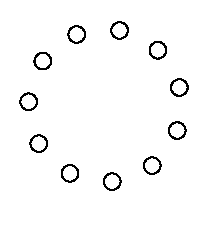
\includegraphics[height=.6\textwidth]{Figuras/A-bloque1}
        \end{minipage}
    \end{subfigure}
    \begin{subfigure}[b]{0.5\textwidth}
        \begin{minipage}{7cm}
        \centering% El subgrafo está centrado
         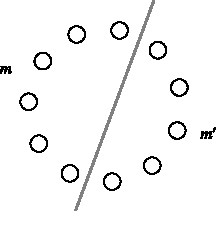
\includegraphics[height=.6\textwidth]{Figuras/A-bloque2}
        \end{minipage}
    \end{subfigure}
    \begin{subfigure}[b]{0.5\textwidth}
        \begin{minipage}{7cm}
        \centering% El subgrafo está centrado
         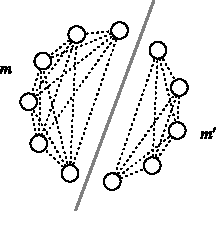
\includegraphics[height=.6\textwidth]{Figuras/A-bloque3}
        \end{minipage}
    \end{subfigure}
    \begin{subfigure}[b]{0.5\textwidth}
        \begin{minipage}{7cm}
        \centering% El subgrafo está centrado
         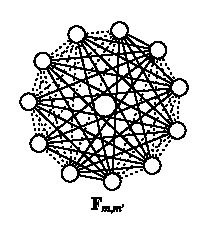
\includegraphics[height=.6\textwidth]{Figuras/A-bloque}
        \end{minipage}
    \end{subfigure}
    \caption{Como se construye un $\DynA$-bloque.}
    \label{figura:2.3}
\end{figure}

El resultado principal de \citep{Barot1999ACO} es que todas las formas unitarias de tipo $\DynA_{n}$ se construyen pegando $\DynA$-bloques sobre un árbol como se explica a continuación:

\begin{enumerate}
\item Se comienza con un árbol $T$ de vértices $\{1, 2, \ldots, t\}$ y a cada vértice $i \in T$ se le asocia un $\DynA$-bloque $\mathcal{B}_{i}$.
 \begin{figure}[H]
    \centering% El subgrafo está centrado
    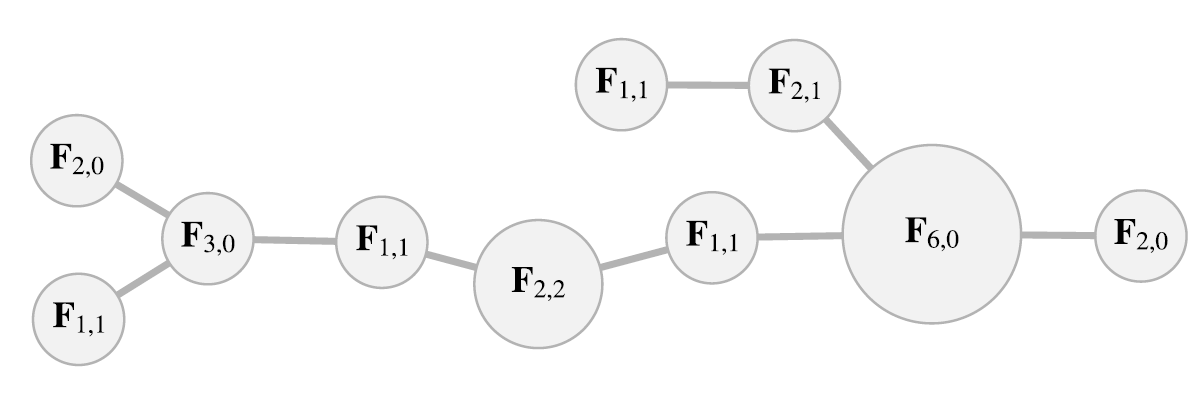
\includegraphics[height=.2\textwidth]{Figuras/graph.png}
\end{figure}
\item A cada arista $i \tikz[baseline=-0.1ex]\draw (0,0.05) -- (1,0.05); j \in T$ se le asocian los vértices $\sigma_{i}\left(i \tikz[baseline=-0.1ex]\draw (0,0.05) -- (1,0.05); j\right) \in \mathcal{B}_{i}$ y $\sigma_{j}\left(i \tikz[baseline=-0.1ex]\draw (0,0.05) -- (1,0.05); j \right)$ de manera que cada función $\sigma_{k}$ sea inyectiva.
 \begin{figure}[H]
    \centering% El subgrafo está centrado
    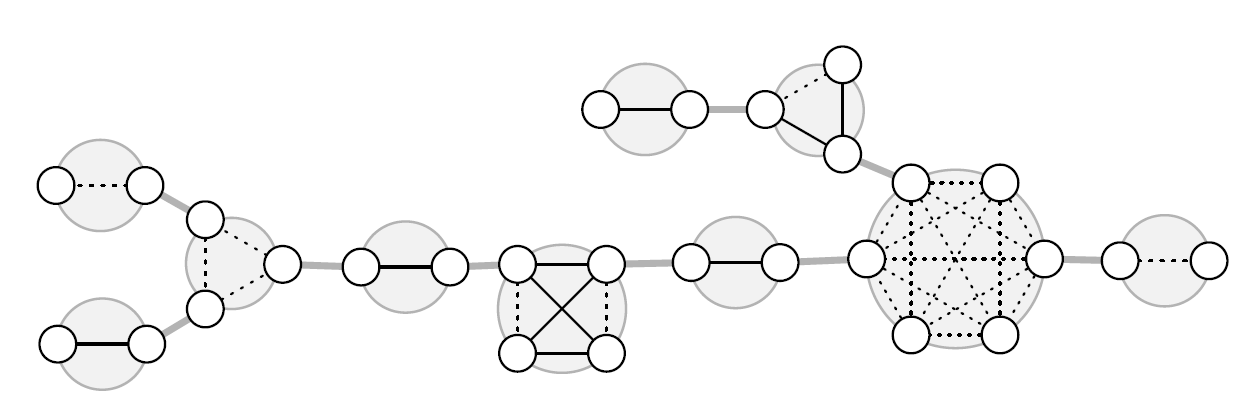
\includegraphics[height=.2\textwidth]{Figuras/graph1.png}
\end{figure}
\item Para cada arista $i \tikz[baseline=-0.1ex]\draw (0,0.05) -- (1,0.05); j \in T$ se identifican los vértices $\sigma_{i}\left(i \tikz[baseline=-0.1ex]\draw (0,0.05) -- (1,0.05); j\right)$ y $\sigma_{j}\left(i \tikz[baseline=-0.1ex]\draw (0,0.05) -- (1,0.05); j\right)$, es decir, se “pegan” para volverse uno solo. Continuando con este ejemplo obtenemos la figura 2.4
 \begin{figure}[H]
    \centering% El subgrafo está centrado
    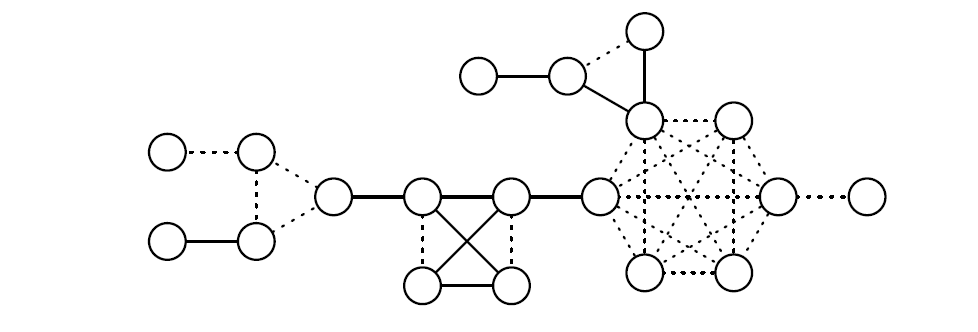
\includegraphics[height=.2\textwidth]{Figuras/graph3.png}
     \caption{Esta gráfica define a una forma de tipo $\DynA_{19}$}
    \label{figura:2.4}
\end{figure}
\end{enumerate}

\textbf{LOS $\DynA$-BLOQUES}

A continuación trataremos de justificar el ensamble de $\DynA$-bloques a partir del siguiente resultado tomado de \citep{article123}:
\begin{theorem}
Si $q_{G}$ es de tipo $\DynA_{n}$, y si $H$ es una subgráfica conexa inducida por $m$ vértices de $G$, entonces $q_{H}$ es de tipo $\DynA_{m}$.
\label{teorema:2.5}
\end{theorem}
Comencemos con un caso especial de gráficas: las gráficas circulares son aquellas en los que cada vértice está conectado con exactamente otros dos vértices. Nos interesa saber cuáles gráficas circulares definen formas cuadráticas de tipo $\DynA_{n}$. Ciertamente $F_{3,0}$ y $F_{2,1}$ son unas de estas (lo podemos comprobar usando el algoritmo \ref{alg:algoritmoInflaciones})\\

Trataremos de simplificar un poco el problema. Las gráficas circulares de la figura 2.5 definen formas $\mathbb{Z}$-equivalentes: podemos pasar de una a otra mediante las matrices elementales $E_{i}^{-1}$ de tamaño $n$. No es difícil comprobar que estas matrices tienen el efecto de intercambiar aristas sólidas con punteadas siempre que estas incidan en el vértice $x_{i}$. De hecho, este mismo razonamiento muestra que toda gráfica circular es equivalente a otra gráfica circular “estandarizada”, que consiste de aristas sólidas y posiblemente una sola arista punteada.\\

\begin{figure}[h]
    \begin{subfigure}[b]{0.3\textwidth}
      \begin{minipage}{7cm}
	\centering% El subgrafo está centrado
	    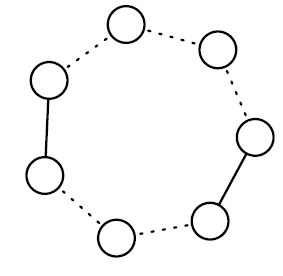
\includegraphics[height=.2\textwidth]{Figuras/graph4.png}
	 \end{minipage}
	\caption{}
     \end{subfigure}
     \begin{subfigure}[b]{0.3\textwidth}
        \begin{minipage}{7cm}
       	 \centering% El subgrafo está centrado
	    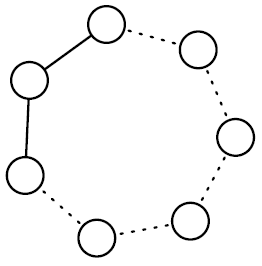
\includegraphics[height=.2\textwidth]{Figuras/graph5.png}
        \end{minipage}
        \caption{}
     \end{subfigure}
     \begin{subfigure}[b]{0.3\textwidth}
        \begin{minipage}{7cm}
       	 \centering% El subgrafo está centrado
	    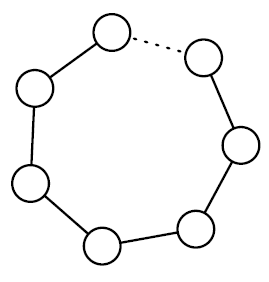
\includegraphics[height=.2\textwidth]{Figuras/graph6.png}
        \end{minipage}
        \caption{}
     \end{subfigure}
     \caption{Ejemplos de gráficas circulares.}
    \label{figura:2.5}
\end{figure}

Podemos descartar a las gráficas que no tienen ninguna arista punteada por que son de tipo $\tilde{A}_{m}$, es decir, no son positivas. Denotemos con $C\left(n\right)$ a el grafo circular de $n$ vértices que tiene exactamente una arista punteada $x_{n} \tikz[baseline=-0.1ex]\draw [dotted] (0,0.05) -- (1,0.05); x_{1}$ y las demás sólidas:

\begin{figure}[h]
   \centering% El subgrafo está centrado
   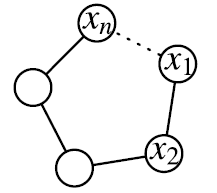
\includegraphics[width=2cm]{Figuras/graph7.png}
\end{figure}

Con el algoritmo \ref{alg:algoritmoInflaciones} podemos comprobar directamente que $C\left(4\right)$ tiene tipo Dynkin $D_{4}$. Si $n \ge 4$, aplicando la inflación $T_{n 1}^{-}$ y borrando el vértice $x_{n}$ de $C\left(n\right)$ se obtiene $C\left(n - 1\right)$, de modo que por inducción y el teorema \ref{teorema:2.5}, todas las gráficas $C\left(n\right)$ con $n \ge 3$ no pueden ser de tipo $\DynA_{n}$. Hemos mostrado el siguiente lema:\\

\begin{lemma}
Las únicas gráficas circulares $G$ tales que $q_{G}$ es de tipo $\DynA_{n}$ son $F_{3,0}$ y $F_{2,1}$.
\label{lema:2.6}
\end{lemma}
 
Una gráfica es $k$-conexa si no existe ningún subconjunto de $k - 1$ vértices tales que su borrado desconecte a la gráfica. Dicho de otro modo, si $\kappa$ denota la cantidad mínima de vértices que es necesario borrar para obtener una gráfica disconexa, entonces $\kappa \geq k$. Por ejemplo, toda gráfica conexa es automáticamente $1$-conexa y toda gráfica completa $K_{n}$ es $k$-conexa para todo $k \in \{1, 2, \dots, n\}$. De hecho, por definición tenemos que si $G$ es una gráfica $k$-conexa entonces también es $\left(k - 1\right)$-conexa, $\left(k - 2\right)$-conexa, etc. Otro ejemplo: las gráficas circulares son gráficas biconexa($2$-conexos). Ahora supongamos que $\textbf{B}_{q}$ es biconexa y que $q$ es de tipo $\DynA_{n}$; mostraremos que $\textbf{B}_{q}$ es un $\DynA$-bloque.\\

Primero mostraremos que $\textbf{B}_{q}$ debe ser una gráfica completa. Supongamos que no es así y sea $S$ el conjunto de vértices más pequeño tal que al borrarlos de $\textbf{B}_{q}$ la gráfica se vuelve disconexa y defínase $\kappa = |S|$. Sabemos que $\textbf{B}_{q}$ es $2$-conexa, y además que la ausencia de la arista $u \tikz[baseline=-0.1ex]\draw (0,0.05) -- (1,0.05); v$ porque $\textbf{B}_{q}$ no es completa) nos permite obtener una gráfica disconexa borrando todos los vértices excepto $u$ y $v$; por lo tanto tenemos que $2 \leq \kappa \leq n-2$. Seleccionamos cualesquiera $\kappa - 2$ vértices del conjunto $S$ y los borramos de la gráfica $\textbf{B}_{q}$ para obtener otra gráfica $\textbf{B}_{q}^{'}$. Por la definición de $S$ sabemos que $\textbf{B}_{q}^{'}$ es una gráfica biconexa pero no triconexa($3$-conexa). Es decir, en $\textbf{B}_{q}^{'}$ existen dos vértices $x$ e $y$ tales que al borrarlos de $B_{q}^{'}$ se obtiene una gráfica de dos componentes conexos $\mathcal{B}_{0}$ y $\mathcal{B}_{1}$. Consideremos el camino más corto $x \leadsto y$ que inicia en $x$ pasa solamente por vértices de $\mathcal{B}_{0}$ y termina en $y$, juntemos este camino con el camino más corto $y \leadsto x$ que inicia en $y$, pasa solamente por vértices de $\mathcal{B}_{1}$ y termina en $x$. Esta unión forma un ciclo $x \leadsto y \leadsto x$, pero habíamos supuesto que $q$ es de tipo $\DynA_{n}$, por tanto el lema \ref{lema:2.6} nos dice que $\textbf{B}_{q}^{'}$ contiene la siguiente subgráfica inducida (sin tomar en cuenta si las aristas son sólidas o punteadas):\\

\begin{figure}[h]
   \centering% El subgrafo está centrado
   \begin{tikzpicture}
   \node (v0) at (1.27, 0.83) {$x_{1}$};
   \node (v1) at (1.27, -0.73) {$x_{2}$};
   \node (v2) at (2.57, 0.83) {$x_{3}$};
   \node (v3) at (2.57, -0.73) {$x_{4}$};
   \draw (v0) -- (v1);
   \draw (v1) -- (v2);
   \draw (v2) -- (v3);
   \draw (v0) -- (v2);
   \draw (v3) -- (v1);
   \end{tikzpicture}
\end{figure}

Aquí $z \in \mathcal{B}_{0}$, $w \in \mathcal{B}_{1}$ y no existe la arista $z \tikz[baseline=-0.1ex]\draw (0,0.05) -- (1,0.05); w$(en otro caso $\textbf{B}_{q}$ seguiría conectada después de quitar los vértices $x$ e $y$). Otra vez mediante el uso del algoritmo \ref{alg:algoritmoInflaciones} se puede demostrar que no importa cuáles aristas sean sólidas o punteadas, esta gráfica no es de tipo $\DynA_{n}$, en contradicción con el teorema \ref{teorema:2.5}; por lo tanto tenemos:\\

\begin{lemma}
Si $q:\mathbb{Z}^{n} \rightarrow \mathbb{Z}$ es una forma unitaria de tipo $\DynA_{n}$ y si $\textbf{B}_{1}$ es una gráfica biconexa, entonces $\textbf{B}_{q}$ es una gráfica completa.
\label{lema:2.7}
\end{lemma}

El siguiente lema se puede leer \textit{entre líneas} en el artículo mencionado; aquí solamente se está recalcando su importancia porque haremos referencia a este lema en capítulos posteriores:

\begin{lemma}
Si toda subgráfica de $\textbf{B}_{q}$ inducida por tres vértices es $F_{3,0}$ o $F_{2,1}$, entonces $\textbf{B}_{q}$ es un $\DynA$-bloque.
\label{lema:2.8}
\end{lemma}

\begin{proof}
Fijemos un vértice $u$ y definamos los conjuntos
\begin{equation*}
\begin{split}
V_{0} & = \{u\} \cup \{v |  \mbox{  existe una arista punteada } u \tikz[baseline=-0.1ex]\draw[dotted] (0,0.05) -- (1,0.05); v\}\\
V_{1} & = \{v |  \mbox{ existe una arista solida } u \tikz[baseline=-0.1ex]\draw (0,0.05) -- (1,0.05); v\}
\end{split}
\end{equation*}
Considérese a otros dos diferentes vértices $v$ y $w$ en $\textbf{B}_{q}$. Por hipótesis tenemos que los vértices $u$, $v$ y $w$ inducen una subgráfica $F_{3,0}$ o $F_{2,1}$. Por la definición de $V_{0}$ y $V_{1}$ concluimos que si dos vértices $v, w$ están en el mismo $V_{i}$ entonces hay una arista punteada $v \tikz[baseline=-0.1ex]\draw[dotted](0,0.05) -- (1,0.05); w$; y en otro caso (están en conjuntos diferentes) hay una arista sólida $v \tikz[baseline=-0.1ex]\draw(0,0.05) -- (1,0.05); w$; por lo tanto $Bq$ es un $\DynA$-bloque.
\end{proof}

Vamos a recapitular lo que hemos visto hasta ahora:\\
\begin{enumerate}
\item El lema \ref{lema:2.7} nos dice que si $q$ es de tipo $\DynA_{n}$ y si $\textbf{B}_{q}$ es biconexa, entonces $\textbf{B}_{q}$ es, de hecho, completa.
\item Pero por el teorema \ref{teorema:2.5} cada subgráfica inducida de $B_{q}$ debe definir otra forma de tipo $\DynA_{n}$.
\item En particular, como $\textbf{B}_{q}$ es completa, el lema \ref{lema:2.6} nos dice que toda subgráfica inducida por cada tres vértices de $B_{q}$ es $F_{3,0}$ o $F_{2,1}$.
\item Entonces, por lema \ref{lema:2.8} concluimos que $\textbf{B}_{q}$ es un $\DynA$-bloque.
\end{enumerate}

Ahora vamos a mostrar el recíproco: que todo $\DynA$-bloque es biconexo y que define una forma de tipo $\DynA_{n}$. La biconexidad es obvia puesto que todo $\DynA$-bloque $F_{m, m}$ es una gráfica completa. Ahora bien, renombremos a los vértices en $V_{0}$ como $x_{1}, x_{2}, \ldots, x_{m}$; y a los de $V_{1}$ como $x_{m+1}, x_{m+2}, \ldots, x_{n}$. Podemos “deshilar” a $\textbf{B}_{q}$ en dos etapas: en la primera quitamos todas las aristas punteadas que hay entre los vértices de $V_{1}$ usando las inflaciones $T_{i i+1}^{-}$ en orden $i = n-1, n-2, \ldots, m+1$ y en la segunda las punteadas que hay en $V_{0}$ usando las inflaciones $T_{i+1 i}^{-}$ en orden $i = 1, 2, \dots, m-1$.\\

Para mostrar que este método de “deshilado” funciona, supongamos que $m \ge 0$ y $m^{'} \ge 0$ y sean $V_{0} = \{x_{1}, \ldots, x_{m}\}$ y $V_{1} = \{x_{m+1}, \ldots, x_{n}\}$ los conjuntos que definen a $F_{m,m^{'}}$ . Sea $x_{r}$ incidente en $x_{n-1}$.

\begin{itemize}
\item Si $x_{r} = x_{n}$ entonces la arista $x_{n-1} \tikz[baseline=-0.1ex]\draw [dotted] (0,0.05) -- (1,0.05); x_{n}$ se sustituye por $x_{n-1} \tikz[baseline=-0.1ex]\draw (0,0.05) -- (1,0.05); x_{n}$.
\item Para todos los $x_{r}$ tales que exista una arista punteada $x_{r} \tikz[baseline=-0.1ex]\draw [dotted] (0,0.05) -- (1,0.05); x_{n-1}$ se tiene que $x_{r} \in V_{1}$ y el arrastre forma una arista sólida $x_{r} \tikz[baseline=-0.1ex]\draw (0,0.05) -- (1,0.05); x_{n}$ que se cancela con la arista $x_{r} \tikz[baseline=-0.1ex]\draw [dotted] (0,0.05) -- (1,0.05); x_{n}$; por lo tanto luego de aplicar $T_{n-1 n}^{-}$ en el vértice $x_{n}$ no incide ninguna arista punteada.
\item Para todos los $x_{r}$ tales que exista una arista sólida $x_{r} \tikz[baseline=-0.1ex]\draw (0,0.05) -- (1,0.05); x_{n-1}$ se tiene que $x_{r} \in V_{0}$ y el arrastre forma una arista punteada $x_{r} \tikz[baseline=-0.1ex]\draw [dotted] (0,0.05) -- (1,0.05); x_{n}$ que se cancela con la arista $x_{r} \tikz[baseline=-0.1ex]\draw (0,0.05) -- (1,0.05); x_{n}$; por lo tanto luego de aplicar $T_{n-1 n}^{-}$ en el vértice $x_{n}$ no incide ninguna arista sólida.
\end{itemize}

De lo anterior concluimos que al aplicar $T_{n-1 n}^{-}$ a $F_{m, m^{'}}$ se obtiene $F_{m, m^{'}-1}$ unida con una arista sólida $x_{n-1} \tikz[baseline=-0.1ex]\draw (0,0.05) -- (1,0.05); x_{n}$; luego entonces por inducción se sigue la sucesión de inflaciones $\left(T_{i i+1}^{-}\right)_{i=n-1}^{m+1}$ sobre el grafo $F_{m,m^{'}}$ produce la gráfica $F_{m,1}$ unido con $x_{m+1} \tikz[baseline=-0.1ex]\draw (0,0.05) -- (1,0.05); \cdots \tikz[baseline=-0.1ex]\draw (0,0.05) -- (1,0.05);  x_{n}$. Un razonamiento similar muestra que la sucesión de inflaciones $\left(T_{i+1 i}^{-}\right)_{i=1}^{m-1}$ aplicadas a $F_{m,1}$ produce $F_{m,m^{'}}$. Por lo tanto el método descrito transforma $F_{m,m^{'}}$ en $\DynA_{m,m^{'}}$. *

\begin{figure}[h]
    \begin{subfigure}[b]{0.3\textwidth}
      \begin{minipage}{7cm}
	\centering% El subgrafo está centrado
	    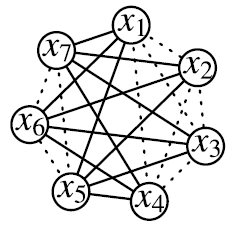
\includegraphics[height=.2\textwidth]{Figuras/graph8.png}
	 \end{minipage}
	\caption{Original}
     \end{subfigure}
     \begin{subfigure}[b]{0.3\textwidth}
        \begin{minipage}{7cm}
       	 \centering% El subgrafo está centrado
	    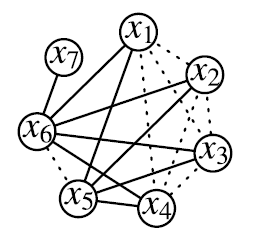
\includegraphics[height=.2\textwidth]{Figuras/graph9.png}
        \end{minipage}
        \caption{$T_{6 7}^{-}$}
     \end{subfigure}
     \begin{subfigure}[b]{0.3\textwidth}
        \begin{minipage}{7cm}
       	 \centering% El subgrafo está centrado
	    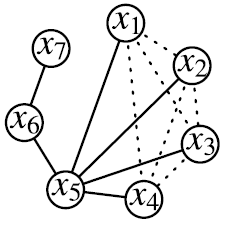
\includegraphics[height=.2\textwidth]{Figuras/graph10.png}
        \end{minipage}
        \caption{$T_{5 6}^{-}$}
     \end{subfigure}
      \begin{subfigure}[b]{0.3\textwidth}
      \begin{minipage}{7cm}
	\centering% El subgrafo está centrado
	    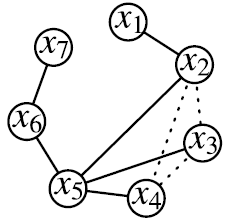
\includegraphics[height=.2\textwidth]{Figuras/graph11.png}
	 \end{minipage}
	\caption{$T_{2 1}^{-}$}
     \end{subfigure}
     \begin{subfigure}[b]{0.3\textwidth}
        \begin{minipage}{7cm}
       	 \centering% El subgrafo está centrado
	    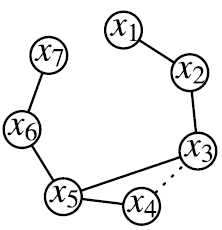
\includegraphics[height=.2\textwidth]{Figuras/graph12.png}
        \end{minipage}
        \caption{$T_{3 2}^{-}$}
     \end{subfigure}
     \begin{subfigure}[b]{0.3\textwidth}
        \begin{minipage}{7cm}
       	 \centering% El subgrafo está centrado
	    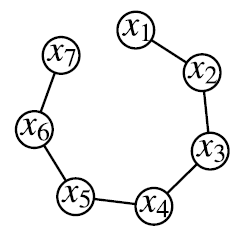
\includegraphics[height=.2\textwidth]{Figuras/graph13.png}
        \end{minipage}
        \caption{$T_{4 3}^{-}$}
     \end{subfigure}
     \caption{Deshilando $F_{4, 3}$}
    \label{figura:2.6}
\end{figure}

Se ha demostrado lo siguiente:
\begin{lemma}
$q$ es una forma unitaria de tipo $\DynA_{n}$ con $\textbf{B}_{q}$ biconexa si y solamente si $\textbf{B}_{q}$ es un $\DynA$-bloque.
\label{lemma:2.9}
\end{lemma}

\textbf{ENSAMBLAJE DE FORMAS $\DynA_{n}$}

Ahora sí tenemos las herramientas necesarias para justificar el ensamble de $\DynA$-bloques. Primero veamos que todo ensamble de $\DynA$-bloques en verdad define una forma unitaria de tipo $\DynA_{n}$.\\

Supongamos que $T$ es el árbol que subyace en un pegado de $\DynA$-bloques. Si este árbol tiene un solo vértice entonces ya acabamos por el lema 2.9 recién mostrado. En otro caso, como $T$ es un árbol, debe haber un vértice $t$ de grado $1$ (podría decirse que t es una hoja del árbol). Entonces el $\DynA$-bloque asociado al vértice $t$, que es $\mathcal{B}_{t} = F_{m, m^{'}}$ , comparte exactamente un vértice $v$ con algún otro $\DynA$-bloque  $\mathcal{B}_{s}$(*). Ahora apliquemos la técnica deshilado explicada justo antes del lema \ref{lemma:2.9}, pero renombrando al vértice $v$ como $x_{m, m^{'}}$ , de manera que este deshilado no afecta en absoluto a ningún otro vértice de $\mathcal{B}_{s}$. Lo que veremos (*) es que ahora del vértice $v$ “cuelga” la siguiente gráfica:

\begin{figure}[h]
    \begin{subfigure}[b]{0.2\textwidth}
      \begin{minipage}{4cm}
	\centering% El subgrafo está centrado
	    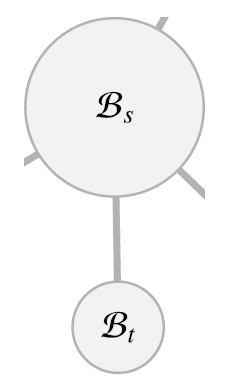
\includegraphics[height=.4\textwidth]{Figuras/graph20.png}
	 \end{minipage}
	 \caption{}
     \end{subfigure}
     \begin{subfigure}[b]{0.2\textwidth}
        \begin{minipage}{4cm}
       	 \centering% El subgrafo está centrado
	    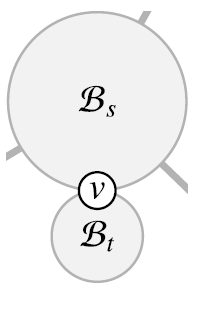
\includegraphics[height=.4\textwidth]{Figuras/graph21.png}
        \end{minipage}
        \caption{}
     \end{subfigure}
     \begin{subfigure}[b]{0.2\textwidth}
        \begin{minipage}{4cm}
       	 \centering% El subgrafo está centrado
	    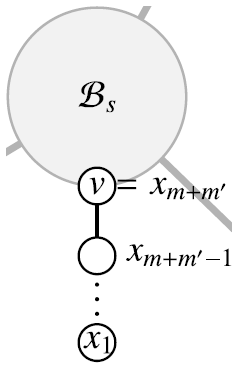
\includegraphics[height=.4\textwidth]{Figuras/graph22.png}
        \end{minipage}
        \caption{}
     \end{subfigure}
      \begin{subfigure}[b]{0.2\textwidth}
      \begin{minipage}{4cm}
	\centering% El subgrafo está centrado
	    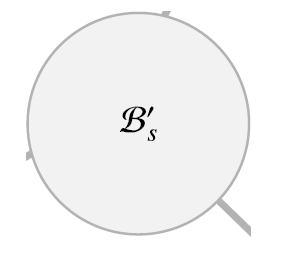
\includegraphics[height=.4\textwidth]{Figuras/graph23.png}
	 \end{minipage}
	 \caption{}
     \end{subfigure}
     \caption{Esquemática de la fusión de dos $\DynA$-bloques}
    \label{figura:2.7}
\end{figure}

\begin{equation*}
x_{m+m^{'}} \tikz[baseline=-0.1ex]\draw (0,0.05) -- (1,0.05); x_{m+m^{'}-1} \tikz[baseline=-0.1ex]\draw (0,0.05) -- (1,0.05); \cdots \tikz[baseline=-0.1ex]\draw (0,0.05) -- (1,0.05); x_{3} \tikz[baseline=-0.1ex]\draw (0,0.05) -- (1,0.05); x_{2} \tikz[baseline=-0.1ex]\draw (0,0.05) -- (1,0.05); x_{1}
\end{equation*}

Esto se parece a lo que se obtiene durante los pasos intermedios para deshilar un $\DynA$-bloque; esto sugiere hacer el proceso inverso, es decir, utilizar las deflaciones.\\

Podemos usar las deflaciones para “tejer” los vértices de $\mathcal{B}_{t}$ en $\mathcal{B}_{s}$ aplicando sucesivamente $T_{i+1, i}$ en orden $i = m + m^{'} - 1, m + m^{'} - 2, \ldots, 3, 2, 1$ (porque precisamente este es el proceso inverso al de deshilado). Cada vez que hacemos esto estamos, en cierto sentido, agregando $x_{i}$ a $\mathcal{B}_{s}$; de manera que al término de estas deflaciones tendremos todos los vértices de $\mathcal{B}_{s}$ y $\mathcal{B}_{t}$ en un mismo $\DynA$-bloque $\mathcal{B}_{s}^{'}$. Así hemos mostrado cómo fusionar dos $\DynA$-bloques del árbol en uno solo, repitiendo este proceso podemos fusionarlos todos, mostrando así que todo ensamble de $\DynA$-bloques es equivalente a un solo $\DynA$-bloque. *

\begin{figure}[h]
    \begin{subfigure}[b]{0.2\textwidth}
      \begin{minipage}{4cm}
	\centering% El subgrafo está centrado
	    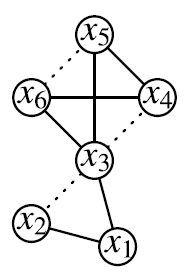
\includegraphics[height=.4\textwidth]{Figuras/graph14.png}
	 \end{minipage}
	\caption{Original}
     \end{subfigure}
     \begin{subfigure}[b]{0.2\textwidth}
        \begin{minipage}{4cm}
       	 \centering% El subgrafo está centrado
	    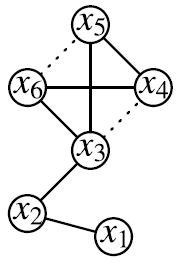
\includegraphics[height=.4\textwidth]{Figuras/graph15.png}
        \end{minipage}
        \caption{$T_{2 3}^{-}$}
     \end{subfigure}
     \begin{subfigure}[b]{0.2\textwidth}
        \begin{minipage}{4cm}
       	 \centering% El subgrafo está centrado
	    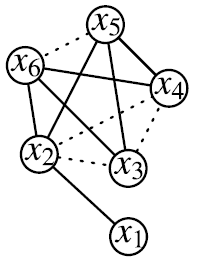
\includegraphics[height=.4\textwidth]{Figuras/graph16.png}
        \end{minipage}
        \caption{$T_{3 2}^{+}$}
     \end{subfigure}
      \begin{subfigure}[b]{0.2\textwidth}
      \begin{minipage}{4cm}
	\centering% El subgrafo está centrado
	    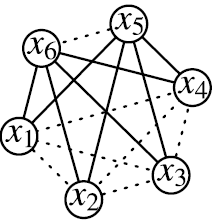
\includegraphics[height=.4\textwidth]{Figuras/graph17.png}
	 \end{minipage}
	\caption{$T_{2 1}^{+}$}
     \end{subfigure}
     \caption{Ejemplo de fusión de dos $\DynA$-bloques}
    \label{figura:2.8}
\end{figure}

\begin{lemma}
Si $G$ es una gráfica construida por un ensamble de árbol de $\DynA$-bloques, entonces $q_{G}$ es de tipo $\DynA_{n}$.
\label{lemma:2.10}
\end{lemma}

Falta mostrar el converso: que si $G$ es una forma unitaria con tipo Dynkin $\DynA_{n}$ entonces se puede construir mediante un ensamble de árbol de $\DynA$-bloques. Una \textbf{componente biconexa} de una gráfica, es una subgrafo biconexo maximal (no contenida propiamente en ninguna otra subgrafo biconexo). La manera más fácil de entender a las componentes biconexos es mediante los \textbf{puntos de articulación}, que son los vértices de la gráfica que al quitarlos la deja desconectada.\\

\begin{figure}[h]
    \begin{subfigure}[b]{0.5\textwidth}
      \begin{minipage}{7cm}
	\centering% El subgrafo está centrado
	    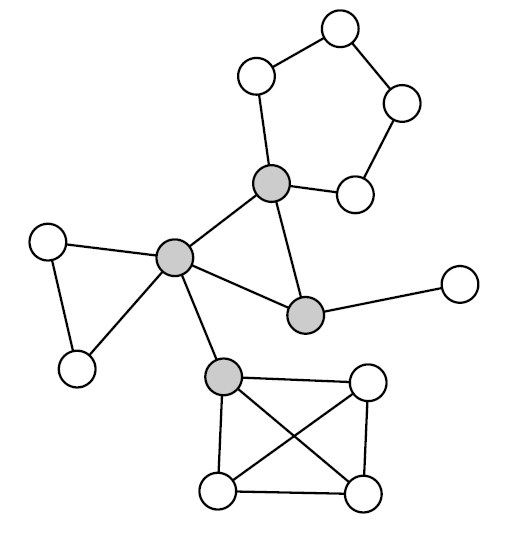
\includegraphics[height=.5\textwidth]{Figuras/graph18.png}
	 \end{minipage}
	\caption{}
     \end{subfigure}
     \begin{subfigure}[b]{0.5\textwidth}
        \begin{minipage}{7cm}
       	 \centering% El subgrafo está centrado
	    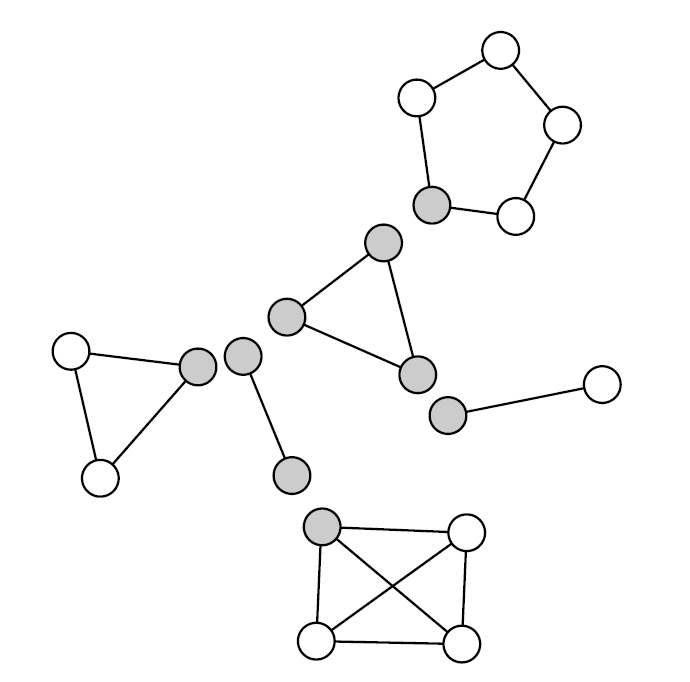
\includegraphics[height=.5\textwidth]{Figuras/graph19.png}
        \end{minipage}
        \caption{}
     \end{subfigure}
     \caption{Una gráfica sus puntos de articulación y componentes biconexas}
    \label{figura:2.9}
\end{figure}

\begin{lemma}
Las componentes biconexas de una gráfica particionan al conjunto de aristas.
\label{lemma:2.11}
\end{lemma}

\begin{proof}
Cada arista es por sí misma una subgrafica biconexa, y por lo tanto pertenece a una subgrafica biconexa maximal; por otro lado ninguna arista puede pertenecer a dos componentes biconexas, por que si este fuera el caso entonces podríamos pegar ambas componentes por medio de la arista que tienen en común, mostrando así que no eran maximales.
\end{proof}

Del teorema \ref{teorema:2.5} y del lema \ref{lemma:2.9} se concluye que si $q$ es de tipo $\DynA_{n}$ entonces las componentes biconexas de $\textbf{B}_{q}$ son $\DynA$-bloques. Supongamos que $\mathcal{B}_{1}, mathcal{B}_{2}, \ldots, \mathcal{B}_{t}$ son las componentes biconexas de $\textbf{B}_{q}$, y formemos una nueva gráfica $T$ de vértices $\{1, 2, \ldots, t\}$, donde cada arista $i \tikz[baseline=-0.1ex]\draw (0,0.05) -- (1,0.05); j$ representa que $\mathcal{B}_{i}$ y $\mathcal{B}_{j}$, con $i \neq j$, tienen un vértice en común (este debe ser un punto de articulación de $\textbf{B}_{q}$). Más aún, si $\mathcal{B}_{i}$ y $\mathcal{B}_{j}$ comparten el vértice $v$ definiremos $\sigma_{i}\left(i \tikz[baseline=-0.1ex]\draw (0,0.05) -- (1,0.05); j\right) = \sigma_{j}\left(i \tikz[baseline=-0.1ex]\draw (0,0.05) -- (1,0.05); j\right) = v$.\\

Debido a la manera en que construimos las funciones $\sigma_{k}$ y la gráfica $T$, tenemos que las siguientes tres afirmaciones son equivalentes:\\

\begin{enumerate}
\item Cada función $\sigma_{k}$ es inyectiva
\item $T$ es un árbol
\item Ningún punto de articulación pertenece a tres o más componentes biconexas
\end{enumerate}

Por lo tanto basta mostrar cualquiera de estas afirmaciones. Mostraremos la tercera afirmación por inducción. Si $\textbf{B}_{q}$ no tiene puntos de articulación, por vacuidad ningún punto de articulación pertenece a tres o más componentes biconexas. Ahora supongamos que $\textbf{B}_{q}$ tiene al menos un punto de articulación $v$; entonces $\textbf{B}_{q} - v$ tiene componentes conexas $\mathcal{C}_{1}, \mathcal{C}_{2}, \ldots, \mathcal{C}_{\ell}$. Defínase $D_{i}$ como la subgráfica de $\textbf{B}_{q}$ inducida por los vértices $V\left(\mathcal{C}_{i}\right) \cup \{v\}$. Por teorema \ref{teorema:2.5} cada $q_{\mathcal{C}_{i}}$ es de tipo $\DynA_{n_{i}}$ y por hipótesis de inducción, cada $C_{i}$ se construye haciendo un ensamble de árbol de $\DynA$-bloques (ningún $\mathcal{C}_{i}$ tiene puntos de articulación que pertenezcan a tres o más componentes biconexas). Ahora, mediante el proceso previamente descrito, deshilemos a cada $\mathcal{C}_{i}$ para convertirlo en un grafo $\DynA_{n_{i}}$ que tenga a $v$ como extremo. Luego entonces $v$ es el centro de una gráfica de estrella de $\ell$ picos y sin aristas punteadas; pero habíamos supuesto que $\textbf{B}_{q}$ es de tipo $\DynA$, de manera que el algoritmo \ref{alg:algoritmoInflaciones} nos dice que $\ell = 2$. Por lo tanto $v$, que es un punto de articulación cualquiera, solamente puede pertenecer a exactamente dos componentes biconexas.\\

Así tenemos el siguente teorema:\\

\begin{theorem}
Una forma unitaria $q$ es de tipo $\DynA_{n}$ si y solamente si $\textbf{B}_{q}$ se construye mediante un ensamble de árbol de $\DynA$-bloques.
\label{teorema:2.12}
\end{theorem}

Sin embargo, para los fines de este trabajo es más conveniente reinterpretar este resultado utilizando otras palabras (pero la demostración es la misma):

\begin{corollary}
Una forma unitaria $q$ es de tipo $\DynA_{n}$ si y solo si $\textbf{B}_{q}$ es conexa, sus componentes biconexas son $\DynA$-bloques y todo punto de articulación pertenece a exactamente dos de estas componentes.
\label{corolario:2.13}
\end{corollary}

\chapter{COMPONENTES TRICONEXAS}

Para esta parte se utilizan los conceptos generados por \citep{hopcroft1973} y mejorados por \citep{Gutwenger2000ALT}.

\section{DIVIDIR UNA GRÁFICA EN COMPONENTES TRICONEXAS}

\subsection{INTRODUCCIÓN}

\paragraph{}
Las propiedades de conectividad de las gráficas forman una parte importante de la teoría de gráficas. En \citep{hopcroft1973} se considera el problema de separar una gráfica en sus componentes triconexas. Un algoritmo para esto es de utilidad para analizar circuitos electricos \citep{1083313} , para determinar si una gráfica es plana \citep{10893101} y para determinar cuando dos gráficas planas son isomorfas \citep{Hopcroft1972}. Un algoritmo para planaridad puede ser usado en el diseño de tablas de circuitos; un algoritmo para isomorfismo de gráficas planas puede ser usado para probar el isomorfismo estructural de compuestos químicos \citep{Lederberg1964DENDRAL64AS} y en nuestro caso para ayudar a clasificar gráficas de Dynkin de tipo $\DynD_{n}$.\\

Una técnica que se ha utilizado para resolver problemas de conectividad es el recorrido primero en profundidad. En \citep{4569669} y \citep{efalgm}, se aplica la búsqueda primero en profundidad para obtener algoritmos eficientes para determinar las componentes biconexas de una gráfica no dirigida y para determinar las componentes fuertemente conexas de una gráfica dirigido. El método también se ha utilizado en un algoritmo eficiente para pruebas de planaridad (\citep{tarjan1971efficient}, \citep{ept}) y en un algoritmo para encontrar dominadores en un grafo de flujo \citep{Tarjan1974FindingDI}. Aquí se aplica la busqueda primeron en profundidad al problema de encontrar las componentes triconexas de una gráfica. Los métodos antiguos para determinar estos componentes requieren $\Theta\left(V^{3}\right)$ pasos o más, si el la gráfica tiene $V$ vértices(\citep{1083313}, \cite{1082941}). El algoritmo descrito aquí requiere sustancialmente utilizamos lña combinacion de los articulos \citep{hopcroft1973} y mejorados por \citep{Gutwenger2000ALT}.\\

Se usa la siguiente notación para especificar límites: si $f$ y $g$ son funciones de $x$, digamos que $f\left(x\right)$ es $\Theta\left(g\left(x\right)\right)$ si, para algunas constantes $k_{1}$ y $k_{2}$, $\left|f\left(x\right)\right| \leq k_{1}\left|g\left(x\right)\right| + k_{2}$ para todo $x$\\

\subsection{Gráficas, conectividad y busqueda en profundidad}

Las definiciones utilizadas aquí se ven \citep{busacker1965finite} y \citep{harary1971graph}. Las componentes triconexas pueden definirse de varias maneras, todas más o menos equivalentes. Los resultados a continuación, se dan sin prueba, siguen de Saunders Maclaine \citep{mac-lane-1937}; estas definiciones se modifican un poco para hacerlos más adecuadas para aplicaciones computacionales.\\

\paragraph{}
Una gráfica $G = \left(\mathscr{V},\mathscr{E}\right)$ consiste de un conjunto $\mathscr{V}$ que contiene $\mathrm{V}$ vertices y un conjunto $\mathscr{E}$ que contiene $\mathrm{E}$ aristas. Si $\mathscr{E}^{`}$ es un conjunto de aristas en $G$, $\mathscr{V}\left(\mathscr{E}^{`}\right)$ es el conjunto de vertices que inciden a uno o más aristas en $\mathscr{E}^{`}$. Si $S$ es un conjunto de vertices en $G$, $\mathscr{E}\left(\mathscr{S}\right)$  es el conjunto de aristas incidentes a al menos un vertice en $S$.

\paragraph{}
Un \textbf{camino} $p:v \overset{\ast}{\Rightarrow} w$ en $G$ es una secuencia de vertices y aristas que van de $v$ a $w$. Un camino es simple si todos sus vertices son distintos. Un camino $p:v \overset{\ast}{\Rightarrow} v$ es un \textbf{ciclo} si todas las aristas son distintas y el único vertice que se repite en $p$ es $v$ y este está al principio y al final de la secuencia de vertices. Un gráfica no dirigida(sin dirección) es conexa(esta conectada) si para cada par de vertices $(v, w)$ existe un camino entre $(v,w)$. Sea $G= \left(\mathscr{V},\mathscr{E}\right)$ y sea $G' =  \left(\mathscr{V}^{`},\mathscr{E}^{`}\right)$ dos gráficas tales que $\mathscr{V}^{`}\subseteq\mathscr{V}$ y $\mathscr{E}^{`}\subseteq \mathscr{E}$ entonces $G^{`}$ es una subgráfica de $G$. Una gráfica con exactamente dos vertices $v,w$ y uno o más aristas $\left(v,w\right)$ se le dice \textbf{enlace}.

\paragraph{}
Un árbol $T$ (dirigido, enraizado) es una gráfica dirigida cuya versión no dirigida es conexa, que tienen un vértice (llamado raíz) y en el que cualquier par de vértices están conectados por exactamente un camino. La relación ``$(v, w)$ es una arista de $T$'' se denota por $v \rightarrow w$. La relación ``hay un camino de $v$ a $w$ en $T$'' se denota por $v \overset{\ast}{\rightarrow}  w$. Si $v \rightarrow w$, donde $v$ es el padre de $w$, y $w$ es un hijo de $v$.Si $v \overset{\ast}{\rightarrow} w$, entonces v en un ancestro de w y w es un descendiente de v. El conjunto de descendientes de un vértice $v$ se denota por $D\left(v\right)$. Todo vértice es ancestro y descendiente de sí mismo. Si $G$ es una gráfica no dirigida, un arbol $T$ es un \textbf{arbol generador} de $G$ si $T$ es un subgráfica de $G$ y $T$ contiene todos los vertices de $G$.

\paragraph{}
Sea $P$ una gráfica no dirigida que consta de dos conjuntos disjuntos de aristas, denotados por $v \rightarrow w$ y $v \rule[1mm]{.1cm}{0.4pt} \rightarrow w$. Supongamos que $P$ satisface las siguientes propiedades:
\begin{enumerate}
\item La subgráfica $T$ que contiene las aristas $v \rightarrow w$ es un árbol generado de $P$.
\item Si $v~ \rule[1mm]{.2cm}{0.4pt} \rightarrow w$, entonces $w \overset{\ast}{\rightarrow}  v$. Es decir, cada arista que no está en el árbol generador $T$ de $P$ conecta el vertice $w$ con uno de sus ancestros $v$ en $T$.
\end{enumerate}
Entonces a $P$ llamaremos árbol de recorrido. Las aristas $v~ \rule[1mm]{.2cm}{0.4pt} \rightarrow w$ las llamaremos aristas de retroceso de $P$.

\paragraph{}
Un gráfica conexa $G$ es \textbf{biconexa} si por cada tripleta de vértices distintos $v$, $w$ y $a$ en $V$, hay un camino $p: v \overset{\ast}{\rightarrow} w$ tal que $a$ no está en el camino $p$. Si hay una tripleta distinta $v$, $w$, $a$ tal que $a$ está en cada camino de  $p :v  \overset{\ast}{\rightarrow} w$, entonces se dice que  $a$ es un \textbf{punto de separación} (o  \textbf{punto de articulación}) de $G$. Podemos particionar las aristas de $G$ de manera que dos aristas están en el mismo bloque de la partición si y sólo si pertenecen a un \textbf{ciclo}. Sea $G_{i} =  \left(V_{i}, E_{i}\right)$ donde $E_{i}$ es el conjunto de aristas en el $i$-ésimo bloque de la partición, y $V_{i} = V\left(E_{i}\right)$. Entonces lo siguiente se cumple:
\begin{enumerate}
\item Cada $G_{i}$ es biconexa.
\item Ningún $G_{i}$ es una subgráfica propia de una subgráfica biconexa de $G$.
\item Cada vértice de $G$ que no sea un punto de articulación de $G$ está exactamente una vez entre los $V_{i}$ y cada punto de articulación está al menos dos veces.
\item Para cada $i, j, i \neq j, V_{i} \cap V_{j}$ contiene como máximo un vértice; además, este el vértice (si existe) es un punto de articulación.
\end{enumerate}
Los subgráficas $G_{i}$ de $G$ se denominan \textbf{componentes biconexas} de $G$. Las componentes biconexas de $G$ son únicas.

\begin{definition}
Sea $G = (V, E)$ una gráfica y sea $H = (W, F)$ una subgráfica de $G$, definimos una relación de equivalencia sobre $E − F$ como sigue:
 \begin{enumerate}
  \item $\forall e \in E - F$, $e \tilde{=} e$
  \item $\forall e, f \in E - F$ con $e: a_{1} \rule[1mm]{.1cm}{0.4pt} b_{1}$ y $f: a_{2} \rule[1mm]{.1cm}{0.4pt} b_{2}$, entonces $e \tilde{=} f$ si y solo si existe un camino de los siguientes tipos:
  \begin{itemize}
   \item $a_{1} \tikz[baseline=-0.1ex]\draw (0,0.05) -- (0.3,0.05); b_{1} \tikz[baseline=-0.1ex]\draw (0,0.05) -- (0.3,0.05); v_{1} \tikz[baseline=-0.1ex]\draw (0,0.05) -- (0.3,0.05); v2 \tikz[baseline=-0.1ex]\draw (0,0.05) -- (0.3,0.05); \cdots \tikz[baseline=-0.1ex]\draw (0,0.05) -- (0.3,0.05); v_{k} \tikz[baseline=-0.1ex]\draw (0,0.05) -- (0.3,0.05); a_{2} \tikz[baseline=-0.1ex]\draw (0,0.05) -- (0.3,0.05); b_{2}$ tal que $b_{1}, v_{1}, \ldots, v_{k}, a_{2} \notin W$
   \item $a_{1} \tikz[baseline=-0.1ex]\draw (0,0.05) -- (0.3,0.05); b_{1} \tikz[baseline=-0.1ex]\draw (0,0.05) -- (0.3,0.05); v_{1} \tikz[baseline=-0.1ex]\draw (0,0.05) -- (0.3,0.05); v2 \tikz[baseline=-0.1ex]\draw (0,0.05) -- (0.3,0.05); \cdots \tikz[baseline=-0.1ex]\draw (0,0.05) -- (0.3,0.05); v_{k} \tikz[baseline=-0.1ex]\draw (0,0.05) -- (0.3,0.05); b_{2} \tikz[baseline=-0.1ex]\draw (0,0.05) -- (0.3,0.05); a_{2}$ tal que $b_{1}, v_{1}, \ldots, v_{k}, b_{2} \notin W$
   \item $b_{1} \tikz[baseline=-0.1ex]\draw (0,0.05) -- (0.3,0.05); a_{1} \tikz[baseline=-0.1ex]\draw (0,0.05) -- (0.3,0.05); v_{1} \tikz[baseline=-0.1ex]\draw (0,0.05) -- (0.3,0.05); v2 \tikz[baseline=-0.1ex]\draw (0,0.05) -- (0.3,0.05); \cdots \tikz[baseline=-0.1ex]\draw (0,0.05) -- (0.3,0.05); v_{k} \tikz[baseline=-0.1ex]\draw (0,0.05) -- (0.3,0.05); a_{2} \tikz[baseline=-0.1ex]\draw (0,0.05) -- (0.3,0.05); b_{2}$ tal que $a_{1}, v_{1}, \ldots, v_{k}, a_{2} \notin W$
   \item $b_{1} \tikz[baseline=-0.1ex]\draw (0,0.05) -- (0.3,0.05); a_{1} \tikz[baseline=-0.1ex]\draw (0,0.05) -- (0.3,0.05); v_{1} \tikz[baseline=-0.1ex]\draw (0,0.05) -- (0.3,0.05); v2 \tikz[baseline=-0.1ex]\draw (0,0.05) -- (0.3,0.05); \cdots \tikz[baseline=-0.1ex]\draw (0,0.05) -- (0.3,0.05); v_{k} \tikz[baseline=-0.1ex]\draw (0,0.05) -- (0.3,0.05); b_{2} \tikz[baseline=-0.1ex]\draw (0,0.05) -- (0.3,0.05); a_{2}$ tal que $a_{1}, v_{1}, \ldots, v_{k}, b_{2} \notin W$
  \end{itemize}
 \end{enumerate}
\end{definition}

\paragraph{}
Si $H = \{\{a, b\}, \emptyset \}$, las clases de equivalencia son llamadas clases de separación relativas al par $\{a, b\}$.
\begin{definition}
Sean $S_{1}, S_{2}, \ldots, S_{k}$, las clases de separación relativas al par $\left(a, b\right)$. Si existe una partición $\left(A, b\right)$ de $\{1, 2, \ldots, k\}$ tal que $\left| E_{1} = \bigcup_{i \in A} S_{i}\right| \geq 2$ y $\left|E_{2} = \bigcup_{j \in B} S_{j}\right| \geq 2$ decimos que $\{a, b\}$ es un par de separación. Veamos esto en el siguiente ejemplo.
\end{definition}

\begin{example}
Sea $G$ el bigrafo y $H=\{\{2, 3\},  \emptyset\}$
  \centering
  \begin{tikzpicture}
  \node (v0) at (1.15, 0.21) {1};
  \node (v1) at (0.08, 0.69) {2};
  \node (v2) at (-0.41, -0.29) {3};
  \node (v3) at (0.62, -0.85) {4};
  \node (v4) at (-0.97, 0.6) {5};
  \draw (v0) -- (v1);
  \draw (v0) -- (v3);
  \draw (v1) -- (v4);
  \draw (v1) -- (v2);
  \draw (v2) -- (v4);
  \draw (v2) -- (v3);
  \end{tikzpicture}
\end{example}

La clase de equivalencia de $2\rule[1mm]{4mm}{0.3mm}5$ es el conjunto:
$$S_{1} = \{2\rule[1mm]{4mm}{0.3mm}5, 5 \hdashrule[1mm]{4mm}{1pt}{1pt} 3\}$$
La clase de equivalencia de $1\hdashrule[1mm]{4mm}{1pt}{1pt} 4$ es el conjunto:
$$S_{2} = \{2 \hdashrule[1mm]{4mm}{1pt}{1pt} 1, 1\rule[1mm]{4mm}{0.3mm}4, 4\rule[1mm]{4mm}{0.3mm}3\}$$
La clase de equivalencia de $2\rule[1mm]{4mm}{0.3mm}3$ es el conjunto:
$$S_{3} = \{2\rule[1mm]{4mm}{0.3mm}3\}$$

Para saber si $\{2,3\}$ es un par de separación hay que encontrar una partición de $\{1, 2, 3\} = A \cup B$, $A \cap B = \{\emptyset\}$ tal que se cumpla que $|E_{1} = \bigcup_{i \in A} S_i| \geq 2$ y $ |E_{2}= \bigcup_{j \in B} S_j| \geq 2$.
En este caso $A = \{1, 3\}$, $B=\{2\}$ es una partición posible que buscamos y entonces $\{2, 3\}$ es un par de separación.\\

Ahora supongamos $\{a, b\}$ es un par de separación. Si $H=\{\{a, b\}, \emptyset\}$ y $S_{1},S_{2}, \ldots, S_{k}$ son las clases de separación del par $\{a, b\}$(las clases de equivalencia definidas por $H$).Sea $A, B$ la partición del conjunto $\{1,2,\ldots,k\}$ tal que $|E_1 = \bigcup_{i \in A} S_i| \geq 2$ y $ |E_{2}= \bigcup_{j \in B} S_j| \geq 2$. Si $H_{1} = (V(E_{1}), E_{1})$ y $H_{2} = (V(E_{2}), E_{2})$ entonces, $V(E_{1}) \cap V(E_{1}) = \{a, b\}$ donde la arista $a\rule[1mm]{4mm}{0.3mm} b$ es llamada arista virtual. Sea $G_{i} = H_{i} + \{a, b\}$ para $i \in \{1, 2\}$. Los $G_{i}$ son las gráficas de separación de $G$ en $\{a, b\}$. A la operación de reemplazar la gráfica $G$ por dos gráficas de separación llamaremos \textbf{separación} de $G$. Debe de haber muchas formas posibles de separar una gráfica, incluso con respecto a un par de separación fijo $\{a, b\}$. Una operación de separación se denota por $s\left(a, b, i\right)$; donde $i$ es un etiqueta que distingue esta operación de separación de otras separaciones. Una arista virtual $\left(a, b\right)$ asociada con la separación $s\left(a, b, i\right)$ se denotará por $\left(a, b, i\right)$. Si $G$ es biconexa, cualquier gráfica de separación de $G$ también es biconexa.

Si hay al menos dos clases de separación, entonces $\{a, b\}$ es una \textbf{par de separación} de $G$ a menos que $(i)$ haya exactamente dos clases de separación y una clase consta de una sola arista, o $(ii)$ hay exactamente tres clases, cada una de las cuales consta de una sola arista.

\paragraph{}
Si $G$ es una gráfica biconexa tal que ningún par $\{a, b\}$ es un par de separación de $G$, entonces $G$ es \textbf{triconexa}. 
\begin{figure}[H]
      \begin{subfigure}[b]{0.3\textwidth}
        \begin{minipage}{5cm}
            \centering% El subgrafo está centrado
            \begin{tikzpicture}
            \node (v0) at (1, 0) {};
            \node (v1) at (-1, 0) {};
            \node (v2) at (0.0, 1) {};
            \draw (v0) -- (v1);
            \draw (v0) -- (v2);
            \draw (v2) -- (v1);
            \end{tikzpicture}
        \end{minipage}
        \caption{Triangulos}
        \label{figura:Triangulos}
        \end{subfigure}
        \begin{subfigure}[b]{0.3\textwidth}
            \begin{minipage}{5cm}
                \centering% El subgrafo está centrado
                \begin{tikzpicture}
                \node(v0) at (0,0) {};
                \node(v1) at (1,0) {};
                \draw (v0) to (v1);
                \draw (v0) to[bend right] (v1);
                \draw (v1) to[bend right] (v0);
            \end{tikzpicture}
        \end{minipage}
        \caption{Enlaces}
        \label{figura:Enlaces}
        \end{subfigure}
        \begin{subfigure}[b]{0.3\textwidth}
            \begin{minipage}{5cm}
            \centering% El subgrafo está centrado
            \begin{tikzpicture}
            \node (v0) at (1, 0.) {};
            \node (v1) at (-1, 0) {};
            \node (v2) at (0.0, -1) {};
            \node (v3) at (0.0, 1) {};
            \draw (v0) -- (v1);
            \draw (v0) -- (v2);
            \draw (v0) -- (v3);
            \draw (v1) -- (v0);
            \draw (v1) -- (v2);
            \draw (v1) -- (v3);
            \draw (v2) -- (v1);
            \draw (v2) -- (v0);
            \draw (v2) -- (v3);
            \draw (v3) -- (v2);
            \draw (v3) -- (v1);
            \draw (v3) -- (v0);
            \end{tikzpicture}
            \end{minipage}
            \caption{Poligonos}
            \label{figura:Poligonos}
            \end{subfigure}
    \caption{Ejemplos de componentes triconexas}
    \label{figura:triconexasEjemplo}
\end{figure}
		
\paragraph{}
Supongamos que separamos una gráfica $G$, las gráficas de separación se dividen, y así sucesivamente, hasta que no sean posibles más separaciones (cada gráfica restante es triconexa). Los gráficas construidas de esta manera se denominan \textbf{componentes de separación} de $G$. Los componentes de separación de una gráfica no son necesariamente únicos.
\begin{lemma}
Sea $G = \left(V, E \right)$ un gráfica con $\left| E \right| \geq 3$. Sea $G_{1}, G_{2}, \ldots G_{m}$ los componentes de separación de $G$. Entonces el número total de aristas en $G_{1}, G_{2}, \ldots , G_{m}$ está delimitado por $3\left| E \right| - 6$.
\label{lema:3.1}
\end{lemma}

\begin{proof}
 El lema se demuestra por inducción sobre el número de aristas de $G$. Si $G$ tiene $3$ aristas, el lema es inmediato, porque $G$ no se puede separar. Supongamos que el lema es cierto para gráficas con $n-1$ aristas y supongamos que $G$ tiene $n$ aristas. Si $G$ no puede ser dividido, el lema es verdadero para $G$. Supongamos, por otro lado, que $G$ se puede separar en $G^{'}$ y $G^{"}$, donde $G^{'}$ tiene $k + 1$ aristas y $G^{"}$ tiene $n - k + 1$ aristas tal que $2 \leq k \leq n - 2$. Por inducción, el número total de aristas en $G_{1}, G_{2}, \ldots G_{m}$ debe estar acotado por $3\left(k + 1\right) - 6 + 3\left(n - k + 1\right) - 6 = 3n - 6$. Así, por inducción, el lema 1 es cierto.
\end{proof}

\paragraph{}
Para obtener las componentes triconexas únicas, debemos volver a unir parcialmente los componentes de separación. Supongamos que $G_{1} = (V_{1},E_{1})$ y $G_{2}=(V_{2},E_{2})$ son dos componentes de separación, ambos con una arista virtual $\left(a, b, i\right)$. Sea
\begin{equation*}
G = \left(V_{1} \cup V_{2}, \left( E_{1} - \{\left(a, b, i\right)\}\right) \cup \left( E_{2} - \{\left(a, b, i\right)\}\right) \right)
\end{equation*}

\paragraph{}
Entonces a $G$ se le llama una \textbf{gráfica de unión} de $G_{1}$ y $G_{2}$; la operación de unión se denotará por $m\left(a, b, i \right)$. La unión es la inversa de la separación; si realizamos un suficiente número de uniones en los componentes divididos de una gráfica, recreamos la gráfica original.

\paragraph{}
Los componentes de separación de una gráfica son de tres tipos: 
\begin{enumerate}
\item enlaces triples de la forma $\left(\{a, b\}, \{\left(a, b\right),\left(a, b\right),\left(a, b\right)\} \right)$ \ref{figura:Enlaces}
\item triangulos de la forma $\left(\{a, b, c\}, \{\left(a, b\right),\left(a, c\right),\left(b, c\right)\}\right)$ \ref{figura:Triangulos}
\item gráficas triconexas \ref{figura:Poligonos}
\end{enumerate}
Sea $G$ una gráfica cuyos componentes de separación son un conjunto de enlaces triples $\mathscr{B}_{3}$, un conjunto de triángulos $\mathscr{F}$ y un conjunto de gráficas triconexas $\mathscr{C}$. Supongamos que los enlaces triples $\mathscr{B}_{3}$ se unen tanto como sea posible para dar un conjunto de enlaces $\mathscr{B}$ y que los triángulos $\mathscr{F}$ se unen tanto como sea posible para dar un conjunto de polígonos $\mathscr{P}$. Entonces el conjunto de gráficas $ \mathscr{B} \cup \mathscr{P} \cup \mathscr{C}$ es el conjunto de componentes triconexas de $G$. Si $G$ es una gráfica arbitraria, las componentes triconexas de las componentes biconexas de $G$ se les llama \textbf{componentes triconexas} de $G$.

\begin{lemma}
Las componentes triconexas de una gráfica $G$ son únicas
\label{lema:3.2}
\end{lemma}

\begin{proof}
Prueba. Ver \citep{mac-lane-1937}, \citep{jEdmonds} y \citep{tarjan-1972}.
\end{proof}

Tomemos como ejemplo el siguiente grafo para mostrar todo el procedimiento.
\begin{figure}[h]
\centering
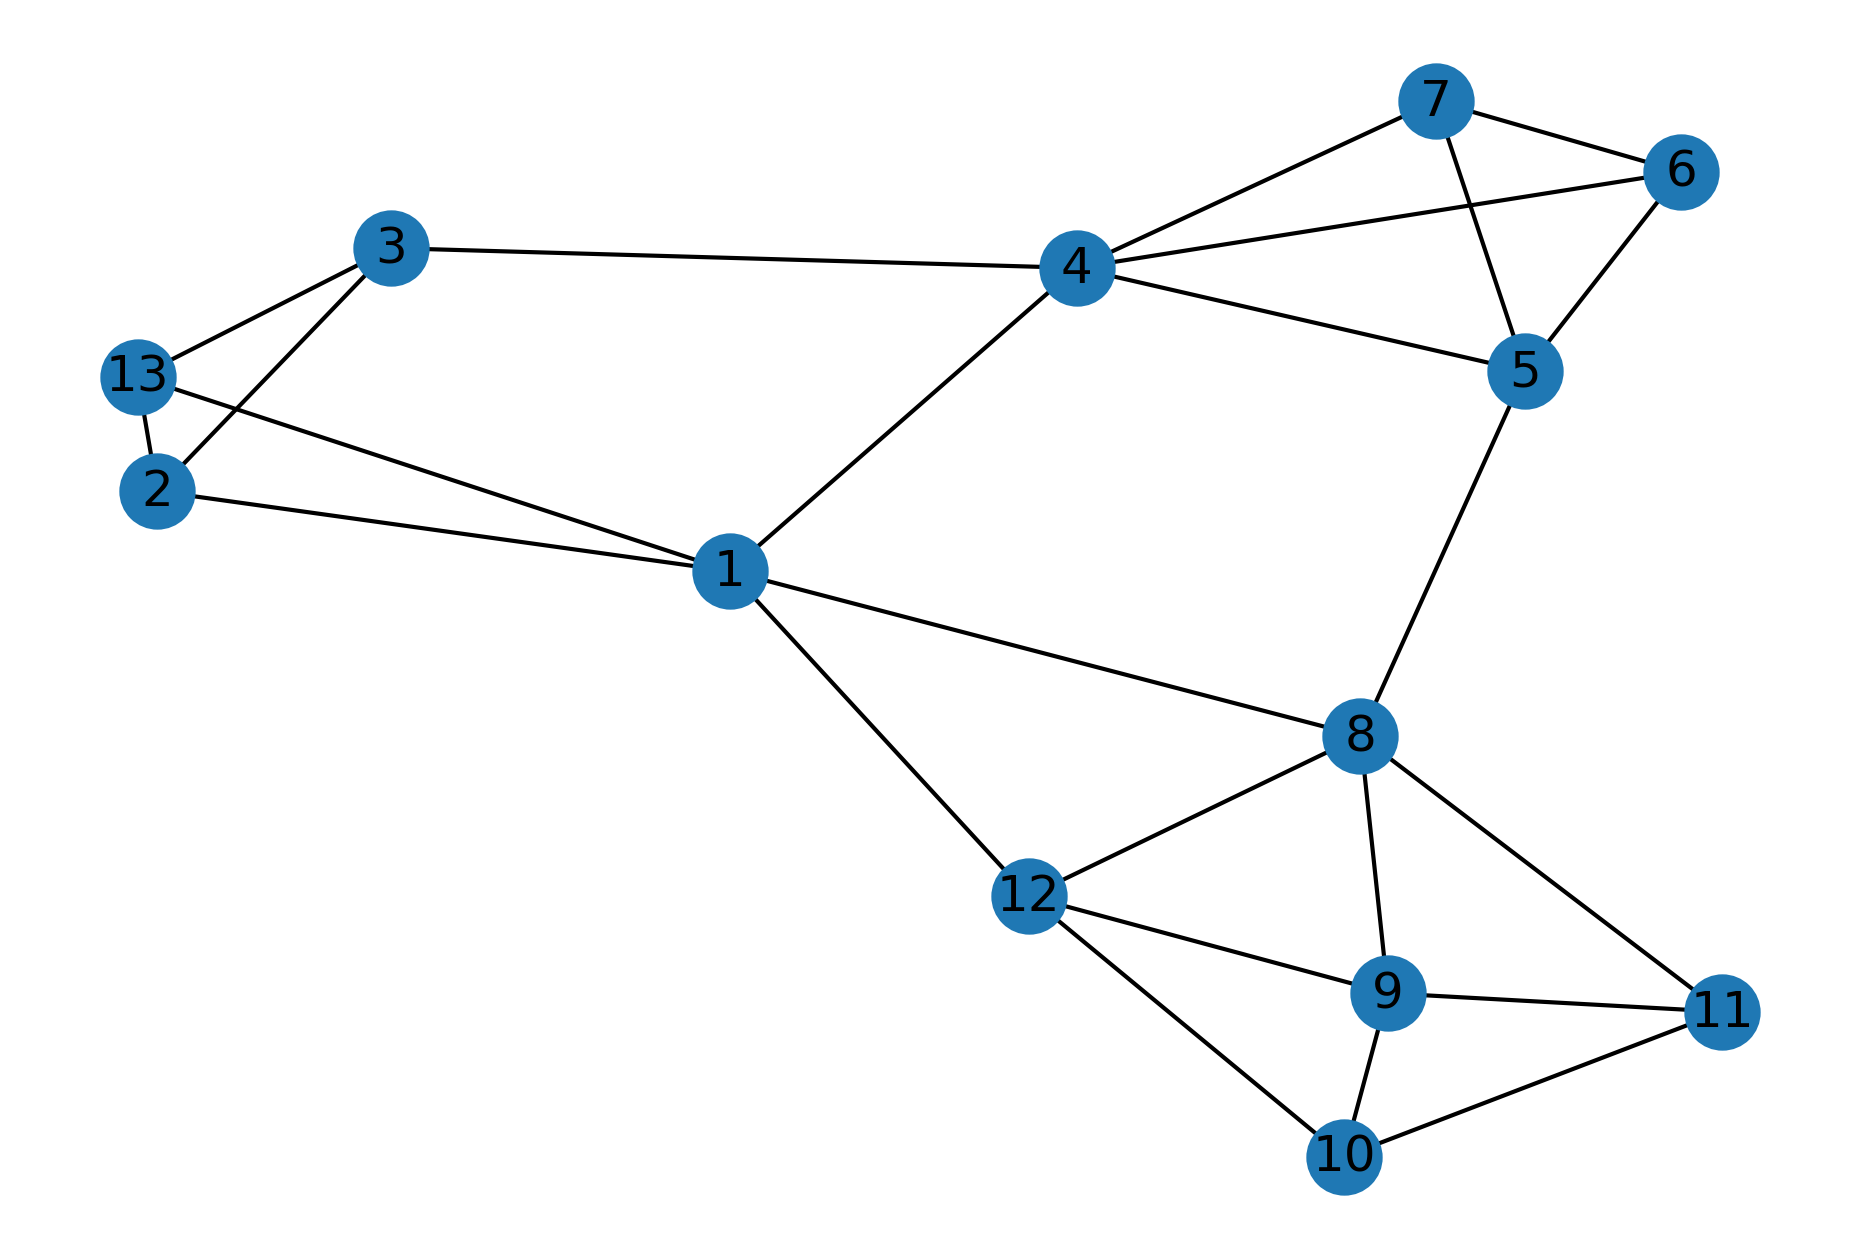
\includegraphics[width=10cm]{Figuras/plotgraph.png}
\caption{Una gráfica biconexa $G$ con pares de separación $(1, 4),(4, 5),(1, 8),(12, 8)$}
\label{figura:3.1}
\end{figure}

\begin{figure}[H]
      \begin{subfigure}[b]{0.3\textwidth}
        \begin{minipage}{7cm}
            \centering% El subgrafo está centrado
            \begin{tikzpicture}[scale=.4]
            \GraphInit[vstyle=Normal]
            %
            \tikzset{VertexStyle/.append style={minimum size=1pt, inner sep=1pt}}
            \Vertex[L=\hbox{$10$},x=2.4209cm,y=5.0cm]{v0}
            \Vertex[L=\hbox{$11$},x=5.0cm,y=2.5701cm]{v1}
            \Vertex[L=\hbox{$12$},x=0.0cm,y=2.4362cm]{v2}
            \Vertex[L=\hbox{$8$},x=2.574cm,y=0.0cm]{v3}
            \Vertex[L=\hbox{$9$},x=2.4254cm,y=2.4944cm]{v4}
            %
            \Edge[](v0)(v1)
            \Edge[](v0)(v2)
            \Edge[](v4)(v0)
            \Edge[](v3)(v1)
            \Edge[](v4)(v1)
            \Edge[](v4)(v2)
            \Edge[](v3)(v4)
            \tikzstyle{EdgeStyle}=[color=red]
            \tikzset{LabelStyle/.style = {fill=white, scale=.6}}
            \Edge[label=$A$](v3)(v2)
            %
            \end{tikzpicture}
        \end{minipage}
      \end{subfigure}
      \begin{subfigure}[b]{0.3\textwidth}
       \begin{minipage}{7cm}
            \centering% El subgrafo está centrado
            \begin{tikzpicture}[scale=.4]
            \GraphInit[vstyle=Normal]
            %
            \tikzset{VertexStyle/.append style={minimum size=1pt, inner sep=1pt}}
            \Vertex[L=\hbox{$12$},x=5.0cm,y=5.0cm]{v0}
            \Vertex[L=\hbox{$8$},x=0.0cm,y=0.0cm]{v1}
            %
            \Edge[](v1)(v0)
            \tikzstyle{EdgeStyle}=[color=red]
            \tikzset{LabelStyle/.style = {fill=white, scale=.6}}
            \Edge[label=$A$, style={bend left}](v1)(v0)
            \Edge[label=$B$, style={bend right}](v1)(v0)
            %
            \end{tikzpicture}
       \end{minipage}
      \end{subfigure}
      \begin{subfigure}[b]{0.3\textwidth}
       \begin{minipage}{7cm}
            \centering% El subgrafo está centrado
            \begin{tikzpicture}[scale=.4]
            \GraphInit[vstyle=Normal]
            %
            \tikzset{VertexStyle/.append style={minimum size=1pt, inner sep=1pt}}
            \Vertex[L=\hbox{$12$},x=5.0cm,y=2.1281cm]{v0}
            \Vertex[L=\hbox{$1$},x=0.0cm,y=0.0cm]{v1}
            \Vertex[L=\hbox{$8$},x=0.51cm,y=5.0cm]{v2}
            %
            \Edge[](v1)(v0)
            \tikzstyle{EdgeStyle}=[color=red]
            \tikzset{LabelStyle/.style = {fill=white, scale=.6}}
            \Edge[label=$C$](v1)(v2)
            \Edge[label=$B$](v2)(v0)
            %
            \end{tikzpicture}
       \end{minipage}
      \end{subfigure}
      \begin{subfigure}[b]{0.3\textwidth}
       \begin{minipage}{7cm}
            \centering% El subgrafo está centrado
            \begin{tikzpicture}[scale=.4]
            \GraphInit[vstyle=Normal]
            %
            \tikzset{VertexStyle/.append style={minimum size=1pt, inner sep=1pt}}
            \Vertex[L=\hbox{$1$},x=0.0cm,y=5.0cm]{v0}
            \Vertex[L=\hbox{$8$},x=5.0cm,y=0.0cm]{v1}
            %
            \Edge[](v0)(v1)
            \tikzstyle{EdgeStyle}=[color=red]
            \tikzset{LabelStyle/.style = {fill=white, scale=.6}}
            \Edge[label=$C$, style={bend left}](v1)(v0)
            \Edge[label=$D$, style={bend right}](v1)(v0)
            %
            \end{tikzpicture}
       \end{minipage}
      \end{subfigure}
      \begin{subfigure}[b]{0.3\textwidth}
       \begin{minipage}{7cm}
            \centering% El subgrafo está centrado
            \begin{tikzpicture}[scale=.4]
            \GraphInit[vstyle=Normal]
            %
            \tikzset{VertexStyle/.append style={minimum size=1pt, inner sep=1pt}}
            \Vertex[L=\hbox{$1$},x=0.0cm,y=5.0cm]{v0}
            \Vertex[L=\hbox{$5$},x=1.4425cm,y=0.0cm]{v1}
            \Vertex[L=\hbox{$8$},x=5.0cm,y=3.8666cm]{v2}
            %
            \Edge[](v1)(v2)
            \tikzstyle{EdgeStyle}=[color=red]
            \tikzset{LabelStyle/.style = {fill=white, scale=.6}}
            \Edge[label=$E$](v0)(v1)
            \Edge[label=$D$](v0)(v2)
            
            %
            \end{tikzpicture}
       \end{minipage}
      \end{subfigure}
      \begin{subfigure}[b]{0.3\textwidth}
       \begin{minipage}{7cm}
            \begin{tikzpicture}[scale=.4]
            \GraphInit[vstyle=Normal]
            %
            \tikzset{VertexStyle/.append style={minimum size=1pt, inner sep=1pt}}
            \Vertex[L=\hbox{$4$},x=2.2676cm,y=0.0cm]{v0}
            \Vertex[L=\hbox{$5$},x=0.0cm,y=2.8922cm]{v1}
            \Vertex[L=\hbox{$6$},x=2.7386cm,y=5.0cm]{v2}
            \Vertex[L=\hbox{$7$},x=5.0cm,y=2.1171cm]{v3}
            %
            \Edge[](v0)(v2)
            \Edge[](v0)(v3)
            \Edge[](v1)(v2)
            \Edge[](v1)(v3)
            \Edge[](v2)(v3)
            \tikzstyle{EdgeStyle}=[color=red]
            \tikzset{LabelStyle/.style = {fill=white, scale=.6}}
            \Edge[label=$F$](v0)(v1)
            %
            \end{tikzpicture}
       \end{minipage}
      \end{subfigure}
      \begin{subfigure}[b]{0.3\textwidth}
       \begin{minipage}{7cm}
            \centering% El subgrafo está centrado
            \begin{tikzpicture}[scale=.4]
            \GraphInit[vstyle=Normal]
            %
            \tikzset{VertexStyle/.append style={minimum size=1pt, inner sep=1pt}}
            \Vertex[L=\hbox{$4$},x=0.0cm,y=0.0cm]{v0}
            \Vertex[L=\hbox{$5$},x=5.0cm,y=5.0cm]{v1}
            %
            \Edge[](v0)(v1)
            \tikzstyle{EdgeStyle}=[color=red]
            \tikzset{LabelStyle/.style = {fill=white, scale=.6}}
            \Edge[label=$F$, style={bend left}](v0)(v1)
            \Edge[label=$G$, style={bend right}](v0)(v1)
            %
            \end{tikzpicture}
       \end{minipage}
      \end{subfigure}
      \begin{subfigure}[b]{0.3\textwidth}
       \begin{minipage}{7cm}
            \centering% El subgrafo está centrado
            \begin{tikzpicture}[scale=.4]
            \GraphInit[vstyle=Normal]
            %
            \tikzset{VertexStyle/.append style={minimum size=1pt, inner sep=1pt}}
            \Vertex[L=\hbox{$1$},x=0.0cm,y=5.0cm]{v0}
            \Vertex[L=\hbox{$4$},x=2.0511cm,y=0.0cm]{v1}
            \Vertex[L=\hbox{$5$},x=5.0cm,y=4.3924cm]{v2}
            %
            \tikzstyle{EdgeStyle}=[color=red]
            \tikzset{LabelStyle/.style = {fill=white, scale=.6}}
            \Edge[label=$H$](v0)(v1)
            \Edge[label=$E$](v0)(v2)
            \Edge[label=$G$](v1)(v2)
            %
            \end{tikzpicture}
       \end{minipage}
      \end{subfigure}
      \begin{subfigure}[b]{0.3\textwidth}
       \begin{minipage}{7cm}
            \centering% El subgrafo está centrado
            \begin{tikzpicture}[scale=.4]
            \GraphInit[vstyle=Normal]
            %
            \tikzset{VertexStyle/.append style={minimum size=1pt, inner sep=1pt}}
            \Vertex[L=\hbox{$1$},x=5.0cm,y=5.0cm]{v0}
            \Vertex[L=\hbox{$4$},x=0.0cm,y=0.0cm]{v1}
            %
            \Edge[](v0)(v1)
            \tikzstyle{EdgeStyle}=[color=red]
            \tikzset{LabelStyle/.style = {fill=white, scale=.6}}
            \Edge[label=$I$, style={bend left}](v0)(v1)
            \Edge[label=$H$, style={bend right}](v0)(v1)
            %
            \end{tikzpicture}
       \end{minipage}
      \end{subfigure}
      \begin{subfigure}[b]{0.5\textwidth}
       \begin{minipage}{7cm}
            \centering% El subgrafo está centrado
            \begin{tikzpicture}[scale=.4]
            \GraphInit[vstyle=Normal]
            %
            \tikzset{VertexStyle/.append style={minimum size=1pt, inner sep=1pt}}
            \Vertex[L=\hbox{$1$},x=5.0cm,y=0.202cm]{v0}
            \Vertex[L=\hbox{$3$},x=0.0cm,y=0.0cm]{v1}
            \Vertex[L=\hbox{$4$},x=2.3629cm,y=5.0cm]{v2}
            %
            \Edge[](v1)(v2)
            \tikzstyle{EdgeStyle}=[color=red]
            \tikzset{LabelStyle/.style = {fill=white, scale=.6}}
            \Edge[label=$J$](v0)(v1)
            \Edge[label=$I$](v0)(v2)
            
            %
            \end{tikzpicture}
       \end{minipage}
      \end{subfigure}
      \begin{subfigure}[b]{0.5\textwidth}
       \begin{minipage}{7cm}
            \centering% El subgrafo está centrado
            \begin{tikzpicture}[scale=.4]
            \GraphInit[vstyle=Normal]
            %
            \tikzset{VertexStyle/.append style={minimum size=1pt, inner sep=1pt}}
            \Vertex[L=\hbox{$13$},x=0.0cm,y=1.6413cm]{v0}
            \Vertex[L=\hbox{$1$},x=5.0cm,y=3.3643cm]{v1}
            \Vertex[L=\hbox{$2$},x=3.4414cm,y=0.0cm]{v2}
            \Vertex[L=\hbox{$3$},x=1.556cm,y=5.0cm]{v3}
            %
            \Edge[](v1)(v0)
            \Edge[](v2)(v0)
            \Edge[](v3)(v0)
            \Edge[](v1)(v2)
            \Edge[](v2)(v3)
            \tikzstyle{EdgeStyle}=[color=red]
            \tikzset{LabelStyle/.style = {fill=white, scale=.6}}
            \Edge[label=$J$](v1)(v3)
            %
            \end{tikzpicture}
       \end{minipage}
      \end{subfigure}
\caption{Componentes de separación de $G$ las componentes triconexas se forma al unir los triangulos $(1, 4, 5)$ y $(1, 5, 8)$}
\label{figura:3.2}
\end{figure}

\paragraph{}
Los algoritmos de gráficas requieren una forma sistemática de explorar una gráfica. En el articulo \citep{hopcroft1973} se utiliza un método llamado \textbf{búsqueda en profundidad}. Para llevar a cabo una búsqueda en profundidad en $G$, se comienza desde algún vértice $s$ y se elije una arista que vaya desde $s$ a otro vertice $w$ en el gráfica, después se marca el vertice $s$ como vistado y se elige ahora $w$ como punto de partida ahora vamos a elegir alguna arista que conecta $w$ cuyo vertice que la conecta a $w$ aun no haya sido visitado si cumple esto elegimos esta arista y marcamos a $w$ como visitado y continuamos así hasta que ya no haya vertices a los cuales visitar. Si $G$ es conexa, cada arista se recorre exactamente una vez*.

\paragraph{}
Si $G$ no es dirigida, una búsqueda sobre $G$ impone una dirección en cada arista de $G$ dada por la dirección en la que se recorre la arista durante la búsqueda. Así la búsqueda convierte $G$ en una gráfica dirigida $G^{'}$.

\begin{lemma}
Sea $P$ la gráfica dirigida generada por una búsqueda en profundidad de una gráfica no dirigida conexa $G$. Entonces $P$ es un árbol de recorrido.
\label{lema:3.3}
\end{lemma}

\begin{proof}
Véase \citep{4569669}.
\end{proof}

\paragraph{}
La búsqueda primero en profundidad es importante porque la estructura de los caminos en un árbol es muy simple. Para implementar una búsqueda en profundidad de una gráfica, usamos un procedimiento recursivo simple que mantiene una pila de los viejos vértices con posiblemente aristas inexploradas. Para representar un gráfica, se utiliza un conjunto de \textbf{listas de adyacencia}, uno para cada vértice. Si $v$ es un vértice la lista de adyacencia $A\left(v\right)$ contiene todos los $w$ tales que $\left(v, w\right)$ es una arista de $G$. Estas listas juntas comprenden una \textbf{estructura de adyacencia} para $G$. Si $G$ no es dirigida, cada arista $\left(v, w\right)$ se representa dos veces, una en $A\left(v\right)$ y otra en $A\left(w\right)$. 

\paragraph{}
\ref{alg:busqueda en profundidad} muestra un procedimiento recursivo para realizar una búsqueda en profundidad. La búsqueda exacta depende del orden de los aristas en las listas de adyacencia. Los números de procedimiento de los vértices del $1$ al $V$ en el orden en que se alcanzan durante el búsqueda, además de identificar arcos y ramas de el árboles de recorrido y aristas de retroceso que nos ayudan mas adelante. La referencia \citep{4569669} da una prueba que el procedimiento es correcto y requiere tiempo $\Theta \left(V + E\right)$ para ejecutarse. Los vértices están numerados de modo que $NUMBER\left(v\right) \le NUMBER\left(w\right)$ si $ v \overset{\ast}{\rightarrow} w$ en el árbol generado.


\begin{algorithm}[!ht]
\DontPrintSemicolon
\tcp{a: declaración vacía}\;
\For{cada $w$ in $A\left(v\right)$}{
 	\If{$NUMBER(w)$ = 0}{
 		marcamos a $(v, w)$ como una rama de el árbol\;
 		$DFS(w, v)$\;
 		\tcp{b: declaración vacía}\;
 	}
 	\ElseIf{($NUMBER(w) < NUMBER(v))$ and (($w \neq u$) or $\neg FLAG(v)$)}{
        marcamos $(v, w)$ como arista de retroceso\;
        \tcp{b: declaración vacía}\;
 	}
 	\If{w=u}{
        $FLAG(v) = false$\:
 	}
}
\DontPrintSemicolon
$n=0$\;
\For{$i=1$ to $V$:}{
    $NUMBER(i) = 0$\;
    $FLAG(i) = True$\;
    }
$DFS(1, 0)$\;
\caption{DFS($v, u$)}\label{alg:busqueda en profundidad}
\end{algorithm}

\paragraph{}
Las declaraciones a, b, c, se reemplazarán cuando se use DFS para calcular otra información sobre el gráfica. En \ref{figura:3.3} representa el arbol formado aplicando DFS y tambien las aristas de backtracking $a \hookrightarrow b$ que son necesarias para nuestro algoritmo. En rojo estan coloreadas las aristas de DFS y en azul el Backtracking de estas aristas y identificar los valores de lowpt1 y lowpt2.

\begin{figure}[H]
\centering
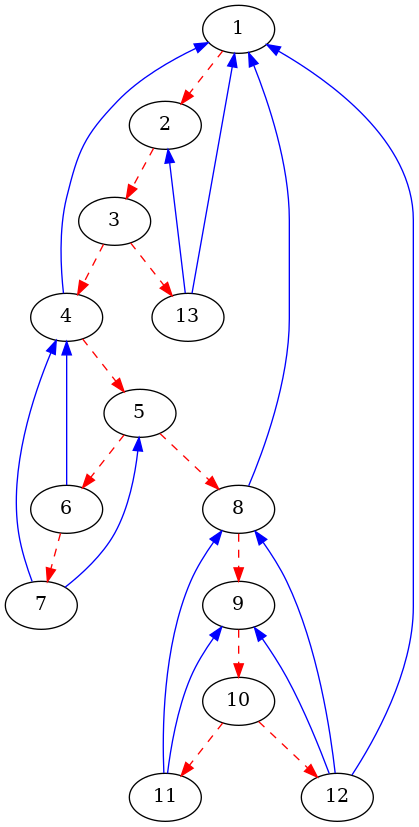
\includegraphics[width=6cm]{Figuras/G2.png}
\caption{Árbol de recorrido generado por la busqueda primero en profundidad de $G$ en \ref{figura:3.1}}
\label{figura:3.3}
\end{figure}

\subsection{La idea de el algoritmo de triconectividad}

\paragraph{}
Esta sección esboza las ideas detrás del algoritmo de triconectividad. Las secciones posteriores desarrollan los componentes detallados. El algoritmo se basa en una idea de Auslander, Parter y Goldstein (\citep{auslander-1961}, \citep{goldstein1963efficient}) para probar la planaridad de los gráficas. La idea de Auslander, Parter y Goldstein da lugar a un algoritmo de tiempo $\Theta\left(V\right)$ para probar la planaridad, si la búsqueda primero en profundidad se utiliza para ordenar los cálculos de (\citep{efalgm}, \citep{ept}). La misma idea da un tiempo $\Theta\left(V + E\right)$ para el algoritmo de encontrar componentes triconexas.

\paragraph{}
Sea $G$ una gráfica biconexo arbitrario. Supongamos que un ciclo $c$ se encuentra en $G$. Cuando se elimina el ciclo de $G$ quedan ciertas piezas conectadas; a estos se les llama \textbf{segmentos}. Auslander y Parter \citep{auslander-1961} demuestran que $G$ es plano si y solo si
\begin{enumerate}
\item Cualquier subgráfica de $G$ que consta de $c$ más un solo segmento es plano.
\item Los segmentos pueden combinarse consistentemente para dar una incrustación plana de todo la gráfica.
\end{enumerate}
Se puede desarrollar un algoritmo de planaridad eficiente a partir de este resultado(\citep{efalgm}, \citep{ept}). A resultado similar se cumple para los pares de separación de $G$, es decir, el siguiente lema.

\begin{lemma}
Sea $G$ una gráfica biconexa y sea $c$ un ciclo en $G$. Seaa $S_{1}, \ldots, S_{m}$ las subgráficas de $G \rule[1mm]{.1cm}{0.4pt} c$ tales que $e_{1}$ y $e_{2}$ son aristas de $S_{i}$ si y sólo si algún camino $p$ en $G$ contiene tanto $e_{1}$ como $e_{2}$ y ningún vértice de $c$ se encuentra entre $e_{1}$ y $e_{2}$ en $p$. Los segmentos $S_{i}$ y el ciclo $c$ particionan las aristas de $G$. Sea $\{a, b\}$ un par de separación de $G$ ,entonces se cumplen las siguientes conclusiones.
\begin{enumerate}
\item Tanto $a$ como $b$ se encuentran en $c$, o bien $a$ y $b$ se encuentran ambos en algún segmento $S_{i}$.
\item Supongamos que tanto $a$ como $b$ están en $c$. Sean $p_{1}$ y $p_{2}$ los dos caminos que componen $c$ los cuales unen $a$ y $b$. Entonces o
\begin{enumerate}
\item Algún segmento $S_{i}$ con al menos dos aristas tiene solo a $a$ y $b$ en común con $c$, y algún vértice $v$ no está en $S_{i}$ ($\{a, b\}$ se le dice par de separación de ''tipo 1''), o
\item Ningún segmento contiene un vértice $v \neq a, b$ en $p_{1}$ y un vértice $w \neq a, b$ en $p_{2}$, $p_{1}$ y $p_{2}$ contienen cada uno un vértice además de $a$ y $b$ ($\{a, b\}$ se le dice par de separación de ''tipo 2'').
\end{enumerate}
\item A la inversa, cualquier par $\{a, b\}$ que satisfaga (a) o (b) es un par de separación.
\end{enumerate}
\label{lema:3.4}
\end{lemma}

\paragraph{}

El lema \ref{lema:3.4} da lugar a un algoritmo recursivo eficiente para encontrar componentes de separación. Encontramos un ciclo en $G$ y determinamos los segmentos formados cuando es eliminado. Probamos cada segmento en busca de pares de separación aplicando el algoritmo recursivamente y probamos el ciclo para pares de separación verificando los criterios en lema \ref{lema:3.4}. La aplicación recursiva del algoritmo requiere encontrar ciclos en subgráficas de $G$ formados por la combinación de un segmento $S_{i}$ y el ciclo inicial $c$.

\paragraph{}
Podemos hacer que este algoritmo sea muy eficiente ordenando los cálculos usando búsqueda en profundidad. Cada llamada recursiva en el algoritmo requiere que encontremos un ciclo en la parte de la gráfica que se va a probar para los pares de separación. Este ciclo constará de un camino simple de aristas las cuales no están en ciclos previamente encontrados más un camino simple de aristas en ciclos no encontrados. Usamos la búsqueda primero en profundidad para separar la gráfica en caminos simples que pueden ensamblarse en estos ciclos. El primer ciclo $c$ consistirá en una secuencia de aristas del árbol seguidos por una arista en $P$, el árbol formado a partir de $G$ por búsqueda primero en profundidad. La numeración de vértices es tal que los vértices están ordenados por número a lo largo del ciclo. Cada segmento consistirá en una sola arista $\left(v, w\right)$ o en una arista $\left(v, w\right)$ de el árbol más un subárbol con raíz $w$, además todas las ramas que salen del subárbol. La búsqueda explora los segmentos en orden decreciente de $v$ y divide cada uno en caminos simples que consisten en una secuencia de ramas de el árbol seguido por una vértice.

\paragraph{}
Encontrar caminos en realidad requiere dos búsquedas porque la búsqueda de caminos debe llevarse a cabo en un orden especial para tener éxito, y ciertos cálculos preliminares son necesarios. La sección sobre cómo encontrar pares de separación describe la proceso de búsqueda de caminos en detalle e incluye una versión del lema \ref{lema:3.4} que caracteriza pares de separación en términos de los caminos generados. La sección de encontrar componentes de separación indica cómo se pueden usar estos resultados para determinar los componentes de separación de una gráfica biconexa en tiempo $\Theta \left(V + E\right)$.

\paragraph{}
Para determinar las componentes triconexas de una gráfica arbitrarias, encontramos las componentes biconexas de la gráfica usando el algoritmo $\Theta \left(V + E\right)$ descrito en \citep{4569669} y \citep{efalgm}. A continuación, los componentes de separación de cada componente biconexa se encuentran utilizando el algoritmo descrito anteriormente y presentado en detalle en el siguiente dos secciones. Esto nos da los componentes de separación de toda la gráfica. El tamaño total de las componentes de separación es $\Theta \left(V + E\right)$, por el lema \ref{lema:3.1}. A continuación identificamos el conjunto de enlaces triples $\mathscr{B}_{3}$ y el conjunto de triángulos $\mathscr{T}$. Para cada uno de estos dos conjuntos, construimos una gráfica auxiliar $S$ cuyos vértices son los elementos del conjunto; dos componentes de separación están unidos por una arista en una gráfica auxiliar si tienen un arista virtual común. Los componentes conectados de $S\left(\mathscr{B}_{3}\right)$ y $S\left(\mathscr{T}\right)$ corresponden a los enlaces y polígonos que son componentes triconexas de $G$. Encontrar estos enlaces y polígonos requiere tiempo $\Theta \left(V + E\right)$. A continuación se muestra un esquema de todo el algoritmo de acuerdo a \citep{Gutwenger2000ALT}.

\section{El algoritmo para encontrar componentes triconexas}

\begin{algorithm}[!ht]
\DontPrintSemicolon
 A: Encontramos las componentes biconexas de $G$;\;
 \For{cada componente biconexa $\mathcal{C}$ de $G$}{
 	B: encontrar los componentes de separación de $C$;\;
 	C: combinar los triangulos en poligonos al encontrar las componentes conexas correspondientes a las gráficas auxiliares;\;
 } 
\caption{TRICONNECTIVITY($G$)}\label{alg:triconexidad}
\end{algorithm}

\paragraph{}
Los pasos A y C requieren tiempo $\Theta \left(V + E\right)$ si se implementan correctamente. La implementación del paso A se describe en \citep{4569669}. El paso difícil es el paso B, cuya implementación se describe en el siguientes dos secciones. Con base en los resultados de estas secciones, toda el algoritmo de triconectividad esta acotado por $\Theta  \left(V + E\right)$.

\subsection{Encontrando pares de separación}

\paragraph{}
Sea $G = \left(\mathscr{V}, \mathscr{E}\right)$ una gráfica biconexa con vértices $V$ y aristas $E$. El problema principal al separar $G$ en sus componentes de separación radica en encontrar sus pares de separación. Esta sección da un criterio simple, basado en la búsqueda primero en profundidad, para identificar los pares de separación de una gráfica. Se deben realizar dos búsquedas en profundidad y algunos cálculos auxiliares. Estos cálculos forman la primera parte del algoritmo de componentes separación y se describen a continuación. Las definiciones de las cantidades lowpt1, ND, etc., utilizadas en el el esquema se dará posteriormente.

\paragraph{Paso 1}
Realice una búsqueda primero en profundidad en el gráfica $G$, convirtiendo $G$ en un árbol $P$. Numeramos los vértices de $G$ en el orden en que se alcanzan durante la búsqueda. Calculamos lowpt1$\left(v\right)$, lowpt2$\left(v\right)$, nd$\left(v\right)$ y padre$\left(v\right)$ para cada vértice $v$ en $P$.

\paragraph{Paso 2}
Construimos una estructura de adyacencia aceptable $A$ para $P$ ordenando las aristas en la estructura de adyacencia de acuerdo con los valores de lowpt1 y lowpt2.

\paragraph{Paso 3}
Realizar una búsqueda en profundidad sobre $P$ utilizando la estructura de adyacencia $A$. Volvemos a numerar los vértices de $A$ desde $V$ a $1$ en el orden en que se examinaron por última vez durante la búsqueda. Particionamos las aristas en caminos simples disjuntos. Recalculamos lowpt1$\left(v\right)$ y lowpt2$\left(v\right)$ utilizando los nuevos números de los vértices. Calculamos A1$\left(v\right)$, deg$\left(v\right)$, y highpt$\left(v\right)$ para cada vértice $v$.

\paragraph{}
Los detalles de estos cálculos aparecen a continuación. Desde los pasos 1, 2 y 3, obtenemos suficiente información para determinar rápidamente los pares de separación de $G$. lema \ref{lema:3.13} da una condición para este propósito.

\paragraph{}
Supongamos que $G$ se explora primero en profundidad, dando un árbol $P$. Sean los vértices de $P$ numerados desde $1$ a $V$ de modo que $v \overset{\ast}{\rightarrow} w$ en $P$ implica que $v \le w$, si identificamos los vértices por su número. Para cualquier vértice $v$ en $P$, sea padre$\left(v\right)$ el padre de $v$ en el árbol de $P$. Sea ND$\left(v\right)$ el número de descendientes de $v$. Sea lowpt1$\left(v\right) = min\left(\{v\} \cup \{w | v \overset{\ast}{\rightarrow} \rule[1mm]{.1cm}{0.4pt} \rightarrow w\}\right)$. Es decir, lowpt1$\left(v\right)$ es el vértice más bajo alcanzable desde $v$ atravesando cero o más ramas de árbol en $P$ seguido de en la mayoría una arista. Sea lowpt2$\left(v\right) = min\left[\{v\} \cup \left(\{w | v \overset{\ast}{\rightarrow} \rule[1mm]{.1cm}{0.4pt} \rightarrow w\} - \{lowpt1 \left(v\right)\}\right)\right]$. Es decir, lowpt2$\left(v\right)$ es el segundo vértice más bajo alcanzable desde $v$ atravesando cero o más ramas de el árbol seguidas por una arista de $P$ como máximo, a menos que lowpt1$\left(v\right) = v$. En este caso, lowpt2$\left(v\right) = v$.

\begin{lemma}
lowpt1$\left(v\right)$ $  \overset{\ast}{\rightarrow} v$ y lowpt2$\left(v\right) \overset{\ast}{\rightarrow}v$ en $P$.
\label{lema:3.5}
\end{lemma}

\begin{proof}
lowpt1$\left(v\right) \leq v$ por definición. Si lowpt1$\left(v\right) = v$, el resultado es inmediato. Si lowpt1$\left(v\right) \le v$, hay una rama $u \rule[1mm]{.1cm}{0.4pt} \rightarrow $lowpt1$(v)$ tal que $v \overset{\ast}{\rightarrow} u$. Como $u \rule[1mm]{.1cm}{0.4pt} \rightarrow $lowpt1$(v)$ es una rama, lowpt1$\left(v\right) \overset{\ast}{\rightarrow} u$. Como $P$ es un árbol, $v \overset{\ast}{\rightarrow} u$ y\\ lowpt1$\left(v\right) \overset{\ast}{\rightarrow} u$, ya sea que $v \overset{\ast}{\rightarrow} $lowpt1$\left(v\right)$ o lowpt1$\left(v\right) \overset{\ast}{\rightarrow} v$. Pero lowpt1$\left(v\right) \le v$. Así debe ser el caso que lowpt1$\left(v\right) \overset{\ast}{\rightarrow} v \overset{\ast}{\rightarrow} u$, y el lema se cumple para lowpt1$\left(v\right)$. La demostración es la misma para lowpt2$\left(v\right)$.
\end{proof}

\begin{lemma}
Supongamos que lowpt1$\left(v\right)$ y lowpt2$\left(v\right)$ se definen en relación con alguna numeración para la cual $v \overset{\ast}{\rightarrow} w$ en $P$ implica NUMERO$\left(v\right) < $ NUMERO$\left(v\right)$. Entonces lowpt1$\left(v\right)$ y lowpt2$\left(v\right)$ identifican vértices únicos independientemente de la numeración usada.
\label{lema:3.6}
\end{lemma}

\begin{proof}
lowpt1$\left(v\right)$ siempre identifica a un ancestro del vertice $v$. Además,\\ lowpt1$\left(v\right)$ es el ancestro con el número más bajo de $v$ con cierta propiedad relativa al árbol $P$. Dado que el orden de los ancestros de $v$ corresponde al orden de sus números, lowpt1$\left(v\right)$ identifica a un único vértice independiente de la númeración, es decir, el primer ancestro de $v$ a lo largo de el camino  $1 \overset{\ast}{\rightarrow} v$ tiene la propiedad deseada(Cualquier numeración satisfactoria asigna $1$ a la raíz de $P$.) La prueba es la misma para lowpt2$\left(v\right)$.
\end{proof}

\paragraph{}
Los valores lowpt de un vértice $v$ dependen solo de los valores lowpt de los hijos de $v$ y en las ramas que salen de $v$; es fácil ver que si los vértices se identifican por número, entonces

\begin{equation*}
lowpt1\left(v\right)= min\left(\{v\} \cup \{lowpt1\left(w\right)| v \rightarrow w\} U \{w| v \rule[1mm]{.1cm}{0.4pt} \rightarrow w\}\right)
\end{equation*}
y
\begin{equation*}
\begin{split}
lowpt2\left(v\right) &=  min(\{v\} \cup ((\{lowpt1\left(w\right)| v \rightarrow w\}\\ 
				   & 	\hspace{0.8cm} \cup \{lowpt2\left(w\right)| v \rightarrow w\} \\
				   &	\hspace{0.8cm} \cup \{w | v \rule[1mm]{.1cm}{0.4pt} \rightarrow  w\}) \newline - \{lowpt1v\})).
\end{split}
\end{equation*}

En el caso de la gráfica anterior los valores de lowpt1 y lowpt2 son los siguientes:\\
\begin{center}
\begin{tabular}{lll}
\toprule
vertice & lowpt1 & lowpt2 \\
\midrule
      1 &      1 &      1 \\
      2 &      1 &      2 \\
      3 &      1 &      2 \\
      4 &      1 &      4 \\
      5 &      1 &      4 \\
      6 &      4 &      5 \\
      7 &      4 &      5 \\
      8 &      1 &      8 \\
      9 &      1 &      8 \\
     10 &      1 &      8 \\
     11 &      8 &      9 \\
     12 &      1 &      8 \\
     13 &      1 &      2 \\
\bottomrule
\end{tabular}
\end{center}

\paragraph{}
También tenemos nd$\left(v\right)= 1 + \sum_{v \rightarrow w} $ ND$\left(w\right)$. Podemos calcular los valores de lowpt, nd y padre para todos los vértices en tiempo $\Theta\left(V + E\right)$ insertando las siguientes declaraciones para las declaraciones a, b, c en DFS. La numeración de los vértices en el orden en que se alcanzan durante la búsqueda garantiza claramente que $v \overset{\ast}{\rightarrow} w$ implica $v \le w$.


\begin{algorithm}[!ht]
\DontPrintSemicolon
a: lowpt1$\left(v\right)$ = lowpt2$\left(v\right)$ = NUMERO$\left(v\right)$; \;
\hspace{0.4cm} ND$\left(v\right)$ = 1 \;
b: \If{lowpt1$\left(w\right) < $ lowpt1$\left(v\right)$}{
	\hspace{0.4cm} lowpt2$\left(v\right) = min\{$lowpt2$\left(v\right), $lowpt2$\left(w\right)\}$\;
	\hspace{0.4cm} lowpt1$\left(v\right) = $ lowpt1$\left(w\right)$\;
	}
\hspace{0.4cm} \ElseIf{lowpt1$\left(w\right) = $ lowpt1$\left(v\right)$}{
   	\hspace{0.4cm} lowpt2$\left(v\right) = min\{$lowpt2$\left(v\right), $lowpt2$\left(w\right)\}$
   }
\hspace{0.4cm} \Else{
   	\hspace{0.4cm} lowpt2$\left(v\right) = \{$ lowpt2$\left(v\right), $lowpt1$\left(w\right)\}$
   }
\hspace{0.4cm} ND$\left(v\right) = $ ND$\left(v\right) + $ND$\left(w\right)$\;
\hspace{0.4cm} FATHER$\left(w\right) = v$\;
c: \If{NUMERO$\left(w\right) < $ lowpt1$\left(v\right)$}{
	\hspace{0.4cm} lowpt2$\left(v\right) = $ lowpt1$\left(v\right)$\;
	\hspace{0.4cm} lowpt1$\left(v\right) = $ NUMERO$\left(w\right)$\;
	}
\hspace{0.4cm} \ElseIf{NUMERO$\left(w\right) = $lowpt1$\left(v\right)$}{
   	\hspace{0.4cm} lowpt2$\left(v\right) = min\{$lowpt2$\left(v\right), $NUMERO$\left(w\right)\}$
   }
\caption{adiciones a DFS($G$)}\label{alg:adicionales a DFS}
\end{algorithm}

\paragraph{}
Verificamos que DFS modificado anteriormente calculará lowpt1, lowpt2, ND y FATHER correctamente en tiempo $\Theta\left(V + E\right)$. (Ver \citep{ept}, \citep{tarjan-1972}.) lowpt1 puede usarse para probar la biconectividad de $G$, como se describe en \citep{4569669}. El siguiente lema es importante.

\begin{lemma}
Si $G$ es biconexa y $v \rightarrow w$, lowpt1$\left(w\right) \le v$ a menos que $v=1$, en cuyo caso lowpt1$\left(w\right) = v = 1$. Además, lowpt1$\left(1\right) = 1$.
\label{lema:3.7}
\end{lemma}

\begin{proof}
Véase [5].
\end{proof}

\paragraph{}
Sea $\phi$ el mapeo de las aristas de $P$ en $\{1, 2, \ldots, 2V + 1\}$ definido por:
\begin{equation*}
\phi(x) =
\begin{cases}
3lowpt1(w) & \text{si $e = v \rightarrow w$ y lowpt$2(w) < v$}\\
3w + 1 & \text{si $e = v \hookrightarrow w$}\\
3lowpt1(w) + 2 & \text{if $e = v \rightarrow w$ y lowpt$2(w) \geq v$}
\end{cases}
\end{equation*}
Sea $A$ una estructura de adyacencia para $P$. $A$ se le dice aceptable si las aristas $e$ en cada lista de adyacencia de $A$ se ordena de forma creciente de acuerdo a $\phi(e)$.

Lo cual da el siguiente resultado de \ref{figura:3.1} en forma de mapeo a cada vertice $1, 2,\ldots, 13$ los vertices adyacentes ordenados de acuerdo al ordenamiento de $\phi$:
\begin{center}
1: [2],\\
 2: [3],\\
 3: [13, 4],\\
 4: [1, 5],\\
 5: [8, 6],\\
 6: [7, 4],\\
 7: [4, 5],\\
 8: [1, 9],\\
 9: [10],\\
 10: [12, 11],\\
 11: [8, 9],\\
 12: [1, 8, 9],\\
 13: [1, 2]
\end{center}
 
\begin{lemma}
Sea P un arbol de una gráfica biconexa $G$ cuyos vértices son numerados de manera que  $v \overset{\ast}{\rightarrow} w$ en $P$ implica $v \le w$. Entonces las estructuras de adyacencia aceptables de $P$ son independientes del esquema de numeración exacto.
\label{lema:3.8}
\end{lemma}

\begin{proof}
Si $v \rightarrow w$ en $P$ entonces por el lema \ref{lema:3.5}, lowpt2$\left(w\right)$ es un ancestro de $w$. Por el lema \ref{lema:3.6} lowpt2$\left(w\right)$ es un vértice fijo independiente de la numeración. Ya que el orden de los ancestros es independiente de la numeración, la cuestión de si lowpt2$\left(w\right)$ es menor que $v$ es independiente de la numeración. Como $G$ es biconexa, si $v \rightarrow w$ en $P$ entonces lowpt1$\left(w\right) \leq v$ por el lema \ref{lema:3.7}. Por el lema \ref{lema:3.5}, lowpt1$\left(w\right)$ es un ancestro de $w$. Dado que lowpt1$\left(w\right) \leq v$, lowpt1$\left(w\right)$ debe ser un ancestro de $v$. Por e lema 3.6, el vertice correspondiente a lowpt1$\left(w\right)$ es independiente de el esquema de numeración. De manera similar si $v \rule[1mm]{.1cm}{0.4pt} \rightarrow w$, entonces por el lema \ref{lema:3.3} y la definición de árbol; $w$ es un ancestro de $v$. Pero el orden de los ancestros de $v$ es idéntico al orden de sus números y este orden es independiente de la numeración. Por lo tanto las estructuras de adyacencia aceptables $A$ para $P$ dependen solo de $P$ y no de la numeración exacta
\end{proof}

Ya despues de tener numeradas las aristas por esta función ordenamos las aristas. Hacemos el recorrido primero en profundidad sobre $G$\\

\paragraph{}
En el paso 3 de los cálculos realizamos una búsqueda en profundidad sobre $P$ usando el estructura de adyacencia aceptable $A$ dada por el paso 2. Esta búsqueda genera un conjunto de caminos de la siguiente manera: cada vez que atravesamos una arista, esta arista la agregamos al  camino que se está construyendo. Cada vez que atravesamos una arista, la arista se convierte en la última arista del camino actual. Así, cada camino consta de una secuencia de ramas del árbol seguidos por un solo vertice. Debido al ordenamiento impuesto a $A$, cada camino termina en el vértice más bajo posible, el camino inicial es un ciclo, y cada camino excepto el primero es simple y sólo tiene en común su vértice inicial y terminal con las anteriores caminos generados (\citep{ept}, \citep{tarjan1971efficient}).

\paragraph{}
Si $p: s \overset{\ast}{\Rightarrow} f$ es un camino generado, podemos formar un ciclo agregando el camino del árbol $f \overset{\ast}{\rightarrow} s$ a $p$. Los ciclos formados de esta manera son los ciclos generados por llamadas recursivas al algoritmo básico de triconectividad explicado en la última sección.

\paragraph{}
Solo necesitamos información mínima sobre los caminos. Sean los vértices de $P$ numerados de manera que $v \overset{\ast}{\rightarrow} w$ implica $v \leq w$. Sea A1$\left(v\right)$ el primer vértice de A$\left(v\right)$. Si $v \rule[1mm]{.1cm}{0.4pt} \rightarrow w$ es la primera rama explorada en el paso 3 que termina en $w$, sea highpt$(w) = v$. Sea deg$\left(v\right)$ el número de aristas que inciden en el vértice $v$. En el paso 3  numeramos los vértices de $V$ a $1$ en el orden en que se examinaron por última vez durante la búsqueda. Esta numeración garantiza que $v \le w$ si $v \overset{\ast}{\rightarrow} w$. El paso 3 también calcula lowpt1$\left(v\right)$, highpt$\left(v\right)$, A1$\left(v\right)$ y deg$\left(v\right)$ con respecto a la nueva numeración.

\paragraph{}
El paso 3 enumera los vértices de $V$ a $1$ en el orden en que se alcanzaron por última vez durante la búsqueda. Sin embargo, a cada vértice en realidad se le debe asignar un número la primera vez que se alcanza, para que el cálculo de highpt se realice correctamente. Para lograr esto, la variable se establece igual a $V$ cuando comienza la búsqueda (afirmación Z). El valor de $i$ disminuye en uno cada vez que se descubre un nuevo vértice (afirmación Y). Así, cuando se alcanza por primera vez un vértice $v$, $i$ es igual al número que desea asignar a $v$ menos el número de vértices a encontrar antes de encontrar $v$ por última vez. Pero los vértices a alcanzar entre el tiempo en que $v$ se examinado por primera vez y el momento en que $v$ se examinar por última vez son solo los descendientes propios de $v$. Por lo tanto, si asignamos el número $i - $nd$\left(v\right) + 1$ a $v$ cuando $v$ se examinar por primera vez (enunciado X), la numeración será correcta.

\begin{tabular}[t]{ll}
1: $1 \rightarrow 2 \rightarrow 3 \rightarrow 13 \hookrightarrow 1$ & 2: $13 \hookrightarrow 2$ \\
3: $3 \rightarrow 4 \hookrightarrow 1$ & 4: $4 \rightarrow 5 \rightarrow 8 \hookrightarrow 1$\\
5: $8 \rightarrow 9 \rightarrow 10 \rightarrow 12 \hookrightarrow 1$ & 6: $12 \hookrightarrow 8$\\
7: $12 \hookrightarrow 9$ & 8: $10 \rightarrow 11 \hookrightarrow 8$\\
9: $11 \hookrightarrow 9$ & 10: $5 \rightarrow 6 \rightarrow 7 \hookrightarrow 4$\\
11: $7 \hookrightarrow 5$ & 12: $6 \hookrightarrow 4$
\end{tabular}\\

Los caminos generados de las aristas ya ordenadas por $phi$ en el paso 3 de la grafica \ref{figura:3.1}.

\paragraph{}
Sea G una gráfica biconexa en el que se han realizado los pasos 1, 2 y 3, dando un árbol $P$ y los conjuntos de valores definidos anteriormente. Sea $A$ con una lista de adyacencia $A\left(v\right)$ la estructura de adyacencia aceptable construida en el paso 2. Sean los vértices de $G$ identificados por los números asignados en el paso 3. Necesitamos una definición más. Si $u \rightarrow v$ y $v$ es la primera entrada en $A\left(u\right)$, entonces a $v$ se le llama el primer \textbf{hijo} de $u$. (Para cada vértice $v$, $A1\left(v\right)$, el primer hijo de $v$, si existe, se calcula en el paso 3). Si $u_{0} \rightarrow u_{1} \rightarrow \cdots \rightarrow u_{n}$ y $u_{i}$ es un hijo primogénito de $u_{i-1}$ para $1 \leq i \leq n$, entonces a $u_{n}$, se le llama el primer descendiente de $u_{0}$. La secuencia de ramas del árbol $u_{0} \rightarrow u_{1} \rightarrow u_{2} \rightarrow \cdots \rightarrow u_{n}$ es parte de un camino generado por el paso 3. Los lemas a continuación dan las propiedades que necesitamos para determinar los pares de separación de $G$.

\begin{lemma}
Sea $A\left(u\right)$ la lista de adyacencia del vértice $u$. Sean $u \rightarrow v$ y $u \rightarrow w$ ramas del árbol con $v$ antes de $w$ en $A\left(u\right)$. Entonces $u \le w \le v$.
\label{lema:3.9}
\end{lemma}

\begin{proof}
El paso 3 numera los vértices de $V$ a $1$ en el orden en que son los últimos examinados en la búsqueda. Si $u \rightarrow v$ se explora antes que $u \rightarrow w$, $v$ se examinarán en último lugar antes de que $w$ se examine en último lugar, y $v$ recibirá un número más alto. Claramente $u$ será el último examinado después de que tanto $v$ como $w$ hayan sido examinados por última vez, por lo que $u$ es el número más pequeño de los tres vértices.
\end{proof}

\begin{lemma}
$A$ es aceptable con respecto a la numeración dada por el paso 3.
\label{3.10}
\end{lemma}

\begin{proof}
El ordenamiento en el paso 2 crea una estructura de adyacencia aceptable para el numeración original. Por el lema \ref{lema:3.9}, $u \rightarrow v$ implica $u \le v$ y por lo tanto por el lema \ref{lema:3.8}, $A$ es aceptable para la nueva numeración.
\end{proof}

\begin{lemma}
Si $v$ es un vértice y $d\left(v\right)$ es el conjunto de descendientes de $v$, entonces $d\left(v\right) = \{x | v \leq x \le v + nd\left(v\right)\}$. Si $w$ es un primer descendiente de $v$, entonces $d\left(v\right)-D\left(w\right) = \{x | v \leq x \le w\}$.
\label{lemma:3.11}
\end{lemma}

\begin{proof}
Supongamos que invertimos todas las listas de adyacencia $A\left(v\right)$ y las usamos para especificar una búsqueda en profundidad de $P$. Los vértices se examinarán por primera vez en sentido ascendente orden de $1$ a $V$, si los vértices se identifican por su número del paso 3. Así a los descendientes de $v$ se les asignan números consecutivos desde $v$ a $v + nd\left(v\right) + 1$. Si $w$ es el primer descendiente de $v$, los vértices en $d\left(w\right)$ se les asignarán números de acuerdo a los vértices en $d\left(v\right) - d\left(w\right)$. Así $d\left(v\right) - d\left(w\right) = \{x | v \leq x \le w\}$.
\end{proof}

\begin{lemma}
Sean $\{a, b\}$ un par de separación en $G$ con $a \le b$. Entonces $a \overset{\ast}{\rightarrow} b$ en el árbol generador $T$ de $P$.1
\label{lema:3.12}
\end{lemma}

\begin{proof}
Como $a \le b$, $a$ no puede ser descendiente de $b$. Supongamos que $b$ no es un descendiente de $a$. Sean $E_{i}$, para $1 \leq i \le k$, las clases de separación con respecto a $\{a, b\}$. Sea $S = \mathscr{V} - D\left(a\right) - D\left(b\right)$. Los vértices $S$ definen un subárbol en $T$ que no contiene a $a$ ni a $b$, por lo que $E\left(S\right)$ debe estar contenido en alguna clase de separación, digamos $E_{1}$. Sea $c$ cualquiera hijo de $a$. $E\left(D\left(c\right)\right)$ debe estar contenido en alguna clase de separación. Pero como $G$ es biconexa, y $a \neq 1$, lowpt1$\left(c\right) < a$, por el Lema 3.7. Por lo tanto, alguna arista incide en un vértice en $S$ y a un vértice en $D\left(c\right)$. Así $E\left(D\left(c\right)\right) \subseteq E_{1}$. Un argumento similar demuestra que las aristas incidentes a cualquier descendiente de $b$ están en $E_{1}$. Pero esto significa que $E_{1} = E$, y entonces ${a, b}$ no puede ser un par de separación.
\end{proof}

\begin{lemma}
Supongamos que $a < b$. Entonces $\{a, b\}$ es un par de separación de $G$ si y solo si ya sea (i), (ii) o (iii) a continuación se cumple:
\begin{enumerate}
\item Hay vértices distintos $r \neq a, b$ y $s \neq a, b$ tales que $b \rightarrow r$, lowpt1$\left(r\right) = a$ , lowpt2$\left(r\right) \geq b$ y $s$ no es un descendiente de $r$. (El par $\{a, b\}$ se le llama par de separación "tipo 1". Los pares de tipo 1 en \ref{figura:3.1} son $(1, 8), (1, 5), (4, 5), (1, 4), (1, 3)$ .
\item Hay un vértice $ r \neq b$ tal que $a \rightarrow r \overset{\ast}{\rightarrow} b$; $b$ es el primer descendiente de $r$ (es decir, $a$, $r$ y $b$ se examinarn en una ruta generada);  $a \neq 1$; cada rama $x \rule[1mm]{.1cm}{0.4pt} \rightarrow y$ con $r \leq x \le b$ y  $a \leq y$ y cada rama $x \rule[1mm]{.1cm}{0.4pt} \rightarrow y$ con $a \le y \le b$ y $b \rightarrow w \overset{\ast}{\rightarrow} x$ tiene lowpt1$\left(w\right) \geq a$. ($\{a, b\}$ se denomina par de separación de "tipo 2". Los pares de tipo 2 en \ref{figura:3.1} son $(8, 12)$)
\end{enumerate}
\label{lema:3.13}
\end{lemma}

\begin{proof}
La parte inversa del lema es más fácil de probar. Supongamos que un par $\{a, b\}$ satisface $\left(i\right)$, $\left(ii\right)$ o $\left(iii\right)$. Sea $E_{i}$ para $1 \leq i \leq k$ las clases de separación de $G$ con respecto a $\{a, b\}$. Supongamos que $\{a, b\}$ satisface $\left(i\right)$. Entonces la arista $\left(b, r\right)$ está contenido en alguna clase de separación, digamos $E_{1}$. Cada rama del árbol con un vértice final en $d\left(r\right)$ tiene el otro extremo en $d\left(r\right) \cup \{a, b\}$. Además, dado que lowpt1$\left(r\right) = a$ y lowpt2$\left(r\right) \geq b$, toda rama con una vértice final en $D\left(r\right)$ tiene la otra vértice final en $D\left(r\right) \cup \{a, b\}$. Por lo tanto, $E_{1}$ consta de todas las aristas con un vértice final en $D\left(r\right)$. No hay otras aristas en $E_{1}$, y las aristas incidentes al vértice $s$ deben estar en alguna otra clase, digamos $E_{2}$. Ya que $E_{1}$ y $E_{2}$ contienen cada uno dos o más aristas, $\{a, b\}$ es un par de separación.\\

Supongamos que $\{a, b\}$ satisface $\left(ii\right)$. Sea $S = d\left(r\right) - d\left(b\right)$. Todas las aristas incidentes a un vértice en $S$ están en la misma clase de separación, digamos $E_{1}$. Dado que $b$ es un primer descendiente de $r$, $S = \{x | r \leq x \le b\}$ por el lema \ref{lema:3.1}. Sean $b_{1}, b_{2}, \ldots, b_{n}$ los hijos de $b$ en el orden ocurren en $A\left(b\right)$. Sea $i_{0} = min\{i | $ lowpt1$\left(b\right) \geq a\}$. Por el ordenamiento impuesto en $A$, $i \le i_{0}$ implica lowpt1$\left(b_{i}\right) \le a$, y $i \geq i_{0}$ implica que lowpt1$\left(b_{i}\right) \geq a$. Por $\left(ii\right)$, cada arista de retroceso con vertice inicial en $S$ tiene su vertice final en $S \cup \{a\}$. También por $\left(ii\right)$, cada arista de retroceso con vertice final en $S$ tiene su vertice inicial en $S \cup \{b\} \cup \left(\bigcup_{i\geq i_{0}}d\left(b_{i}\right)\right)$. Cada arista con un vertice final en $d\left(b\right)$, $i \geq i_{0}$, tiene su otro extremo en $S \cup \{a, b\} \cup d\left(b\right)$. Así la clase $E_{1}$ contiene al menos todas las aristas con un vertice final en $S$ y como máximo todas las aristas con un vertice final en $S \cup (\bigcup_{i\geq i_{0}}d(b_{i}))$. Como $a \neq 1$, las aristas incidentes a la raíz de $P$ no pueden estar en $E_{1}$ y por lo tanto $\{a, b\}$ es un par de separación.\\

Ahora debemos demostrar la parte directa del lema. Por \ref{lema:3.12}, $a \overset{\ast}{\rightarrow} b$. Sea $E_{i}$, para $1 \leq i \leq k$, las clases de separación de $G$ con respecto a $\{a, b\}$. Sea $v$ el hijo de $a$ tal que $a \rightarrow v  \overset{\ast}{\rightarrow} b$, $S =  d\left(v\right) - d\left(b\right)$, y $X = V - d\left(a\right)$. (O $S$ o $X$ o ambos pueden estar vacíos.). $E\left(S\right)$ y $E\left(X\right)$ están contenidos cada uno en una clase de separación, digamos $E\left(S\right) \subseteq E_{1}$ y $E\left(X\right) \subseteq E_{2}$.\\

Sea $a_{i} \neq v$ un hijo de $a$. Si $a$ tiene un hijo así, lowpt1$\left(a\right) \le a$. Esto significa que $E\left(d\left(a_{i}\right)\right) \subseteq E_{2}$. Sean $Y = X \cup \left(\bigcup_{i}d(a_{i}\right)$. Sean $b_{1}, b_{2}, \ldots b_{n}$ los hijos de $b$ en el orden en que aparecen en la lista de adyacencia de $b$. Sea $E\left(d\left(b\right)\right)$ el conjunto de aristas con vertice final en $d\left(b\right)$. Las clases de separación deben ser uniones de los conjuntos $E\left(S\right), E\left(Y\right)$, $\{\left(a, b\right)\}, E\left(d\left(b_{1}\right)\right), E\left(d\left(b_{2}\right)\right), \cdots E\left(d\left(b_{n}\right)\right)$.\\

Si $E\left(d\left(b\right)\right) = E_{j}$ para algún $i$ y $j$, entonces lowpt1$\left(b_{i}\right) = a$ ya que $G$ es biconexo y esto significa que lowpt1$\left(b_{i}\right) \le b$ por el Lema 3.7. También, lowpt2$\left(b_{i}\right) \geq b$. Ya que $\{a, b\}$ es un par de separación, debe haber una clase de separación distinta de $E_{j}$ y $\{\left(a, b\right)\}$. Por tanto, existe un vértice $s$ tal que $s \neq a$, $s \neq b$, y $s \notin d\left(b_{i}\right)$. Esto significa que $\{a, b\}$ satisface $\left(i\right)$ donde $r$ es $b_{i}$.\\

Supongamos ahora que ninguna $E\left(d\left(b\right)\right)$ es una clase de separación. Sea $i_{0} = min\{i | $ lowpt1$\left(b_{i}\right) \geq a\}$. Si $i \geq i_{0}$, entonces como $G$ es biconexo, debe ser el caso que lowpt1$\left(b\right) \le b$, y estas clases de separación son $E_{1} = E\left(S\right) \cup \left(\bigcup_{i \geq i_{0}}E\left(d\left(b_{i}\right)\right)\right)$,\\ $E_{2} = E\left(Y\right) \cup \left(\bigcup_{i \le i_{0}} E\left(d\left(b_{i}\right)\right)\right),~ E_{3} = \{(a, b)\}$. ($E_{3}$ puede estar vacío.) Tenemos $v \neq b$ ya que $\{a, b\}$ no es un par de tipo 1 y $a \neq 1$ ya que $E_{2}$ no es vacío. Si $x \rule[1mm]{.1cm}{0.4pt} \rightarrow y$ es una rama con $v \leq x \le b$, entonces $x \in S,~ \left(x, y\right) \in E_{1}$, y $a \geq y$. Si $x \rule[1mm]{.1cm}{0.4pt} \rightarrow y$ es una rama con $a \le y \le b$ y $b \rightarrow b_{i} \overset{\ast}{\rightarrow} x$, entonces $y \in S,~ \left(x,y\right) \in E_{1}$ y $ i \geq i_{0}$, lo que significa que lowpt1$\left(b_{i}\right) \geq a$. Debemos verificar una condición más para demostrar que $\left(ii\right)$ se cumple, es decir, que $b$ es un primer descendiente de $v$. Dado que $G$ es biconexa, lowpt1$\left(v\right) \le a$. Por lo tanto alguna arista con vertice inicial $d\left(v\right)$ tiene un vertice final $ < a$. Por el ordenamiento impuesto a $A$S y la definición de un primer descendiente, existe alguna arista de retroceso $x \rule[1mm]{.1cm}{0.4pt} \rightarrow y$ con $x \in d\left(v\right)$ y $y \le a$ tal que $x$ es el primer descendiente de $v$. Si $b$ no fuera el primer descendiente de $v$, entonces $x$ estaría en $S$, y $E_{1}$ y $E_{2}$ no podrían ser clases de separación distintas. Por lo tanto, $b$ es un primer descendiente de $v$, y $\left(ii\right)$ se cumple con $r = v$. Esto completa la prueba de la parte directa del lema.
\end{proof}

\paragraph{}
Vale la pena considerar cuidadosamente \ref{lemma:3.13} y su demostración. El lema da tres condiciones fáciles de aplicar para pares de separación. Las condiciones $\left(i\right)$ y $\left(ii\right)$ identifican los pares de separación no triviales de la gráfica. La condición $\left(iii\right)$ maneja aristas múltiples. La condición $\left(i\right)$ requiere que se realice una prueba simple en cada rama del árbol $P$. Por lo tanto, la prueba de pares de tipo 1 requiere tiempo $\Theta\left(V\right)$. La prueba de pares de tipo 2 es algo más difícil, pero se puede hacer en tiempo $\Theta\left(V + E\right)$ usando otra búsqueda primero en profundidad. Sea $\{a, b\}$ un par de tipo 2 que satisfaga $a \rightarrow r \overset{\ast}{\rightarrow} b$ y $i_{0} = min\{i | lowpt2\left(b_{i}\right) \geq a\}$, donde $b_{1}, b_{2}, \ldots, b_{n}$, son los hijos de $b$ en el orden en que aparecen en $A\left(b\right)$. Entonces una clase de separación con respecto a $\{a,b\}$ es $E\left(\{x | r \leq x \le b_{i_{0}} + nd\left(b_{i_{0}}\right)\} - \{b\}\right)$. Esto se sigue de la demostración de \ref{lema:3.13}. La nueva numeración satisface la condición un tanto extraña en \ref{lema:3.9} por lo que hace fácil determinar la clases de separación y separar la gráfica cuando se encuentra un par de separación. Un algoritmo para encontrar los componentes de separación basado en \ref{lema:3.13} se da en el siguiente sección.

\subsection{Encontrando componentes de separación}

\paragraph{}
Encontramos los componentes de separación al examinar los caminos generados en orden y probamos los pares de separación con \ref{lema:3.13}. Los pares de separación serán de varios tipos. Pares de tipo 1 son mas faciles de reconocer. También lo son los pares de tipo 2 $\{a, b\}$, donde $a \rightarrow v \rightarrow b$ y $v$ tiene grado dos. Otros pares de tipo 2 son algo más difíciles de reconocer. Sea $c$ el primer camino generado (un ciclo). El ciclo consta de un conjunto de aristas del árbol $1 \rightarrow v_{1} \rightarrow v_{2} \rightarrow \cdots \rightarrow v_{n}$ seguido de una rama $v_{n} \rule[1mm]{.1cm}{0.4pt} \rightarrow 1$. La numeración de los vértices es tal que $1 \le v_{1} \le \cdots \le v_{n}$. Cuando se elimina $c$, la gráfica se divide en varias partes conectadas, llamadas \textbf{segmentos}. Cada segmento consta de una sola arista $\left(v_{i}, v_{j}\right)$ o de una arista del árbol $\left(v_{i}, w\right)$ más un subárbol con raíz $w$ más todas las aristas que salen del subárbol. El orden del camino generado es tal que todas las rutas en un segmento se generan antes que las rutas en cualquier otro segmento, y los segmentos se exploran en orden decreciente de $v_{i}$.\\
Supongamos que repetimos la búsqueda del camino, usándola ahora para encontrar los componentes de separación. Mantendremos una pila de aristas, agregando aristas a esta pila a medida que retrocedemos sobre ellos durante la búsqueda. Cada vez que encontramos un par de separación, eliminamos un conjunto de aristas de la pila correspondiente a un componente de separación. Agregamos una arista virtual correspondiente a la separación tanto al componente como a la pila de aristas. Nosotros también necesitamos actualizar varias piezas de información, ya que los padres de vértices y los grados de los vértices pueden cambiar cuando se divide una gráfica. El camino completo de la búsqueda creará un conjunto completo de componentes de separación. Unir los componentes de separación para dar los componentes triconexos es el paso final.\\
Para identificar los pares de tipo 2, mantenemos una pila (llamada tstack) de tripletas $\left(h, a, b\right)$. El par $\{a, b\}$ es un posible par de tipo 2 y $h$ denota el vértice numerado más grande en el componente de separación correspondiente. Los pares están en orden anidado en la pila; es decir, si $v_{i}$ es el vértice actual que está siendo examinado por la búsqueda de ruta y $\left(h_{1}, a_{1}, b_{1}\right), \left(h_{2}, a_{2}, b_{2}\right), \cdots, \left(h_{k}, a_{k}, b_{k}\right)$ están en tstack, entonces $a_{k} \leq a_{k-1} \leq \cdots \leq a_{2} \leq a_{1} \leq v_{i} \leq b_{1} \leq b_{2} \leq \cdots \leq b_{k}$. Además, todos los $a_{j}$ y $b_{j}$ son vértices. en el ciclo c.\\

Se actualiza tstack de las siguientes maneras:\\

\begin{enumerate}
\item Cada vez que recorremos un nuevo camino $p: s \overset{\ast}{\Rightarrow} f$, borramos todos las tripletas $(h_{j}, a_{j}, b_{j})$ encima de la pila con $a \ge f$. Si $p$ tiene un segundo vértice $v \neq f$, sea $x = v + ND\left(v\right) + 1$. De lo contrario, sea $x = s$. Sea $y = max\{h_{j} | triple(h_{t}, a_{t}, b_{t})$ que se eliminó de tstack$\}$. Si $(h_{k}, a_{k}, b_{k})$ fue la última tripleta eliminada, agregamos $\left(max\left(x, y\right), f, s\right)$ a la pila. Si no se eliminó una tripleta, agregamos $\left(x, f, s\right)$ a la pila.
\item Cuando retrocedemos sobre una rama del árbol $v_{i} \rightarrow v_{i+1}$ con $v \neq 1$, borramos todos entradas $(h_{j}, a_{j}, b_{j})$ encima de tstack que satisfacen highpt$\left(v_{i}\right) > h_{j}$. esta prueba es necesaria para garantizar que las entradas que no correspondan a los pares de tipo 2 no se acumulan en tstack.
\end{enumerate}

Usamos tstack para encontrar pares de separación de la siguiente manera: siempre que busquemos hacia atrás a lo largo de una rama del árbol $v_{i} \rightarrow v_{i+1}$ durante la búsqueda de ruta, examinamos la tripleta superior en $\left(h_{1}, a_{1}+, b_{1}\right)$ en tstack. Si $v \neq 1$, $a = v_{i}$, y $a \neq$ padre$(b_{i})$, $\{a_{1},b_{1}\}$ es un par de separación de tipo 2. Si deg$\left(v + 1\right) = 2$ y $v_{i+1}$ tiene un hijo, entonces $v_{i}$ y el hijo de $v_{i+1}$ forman un par de separación tipo 2. Dividimos los componentes correspondientes a los pares de tipo 2 hasta que estas dos condiciones no nos den más componentes. (Simultáneamente, probamos los componentes correspondientes a múltiples aristas y los dividimos.) Luego aplicamos el Lema 3.13 para probar si $\{v,$ lowpt1$\left(v+ 1\right)\}$ es un par de tipo 1, dividiendo un componente si es necesario. (De nuevo, tenemos que comprobar si hay un componente de múltiples aristas).\\

Manejamos la parte recursiva del algoritmo de la siguiente manera: recorremos una ruta $p: s \overset{\ast}{\Rightarrow} f$ que comienza en $c$ significa que la búsqueda está entrando a un nuevo segmento. El vértice $f$ debe ser el vértice más bajo en el segmento por el orden impuesto en el búsqueda de caminos. Después de actualizar tstack como se describe arriba, si $p$ contiene más de una arista, colocamos un marcador de fin de pila en tstack y continuamos encontrando caminos. Esto corresponde a una llamada recursiva de la triconectividad básica del algoritmo. Cuando retrocedemos sobre el primer arista de $p$, eliminamos todas las entradas de tstack hasta el marcador de fin de la pila. esto corresponde a apareciendo de la recursividad.

\paragraph{}
Un punto más necesita explicación: la razón por la que usamos lowpt2 así como lowpt1 para construir $A$, la estructura de adyacencia aceptable que determina el orden de búsqueda de caminos. Este paso es necesario para que todas las aristas múltiples sean manejadas correctamente. Supongamos que $v$ es un vértice, y $w_{1}, w_{2}, \ldots, w_{k}$ son los hijos de $v$ tales que lowpt1$(w_{i}) = u$. Además, supongamos que $v \rule[1mm]{.1cm}{0.4pt} \rightarrow u$. Sea la $w_{i}$ ordenada como en $A\left(v\right)$. Hay algún $i_{0}$ tal que $i \leq i_{0 } \Rightarrow$ lowpt2$\left(w_{i}\right) \le v$ y $i \ge i_{o} \Rightarrow$ lowpt2$\left(w_{i}\right) \geq v$. En $A\left(v\right)$, $u$ aparecerá después de el $w_{i}$ con $1 \leq i \leq i_{0}$. Si $i \ge i_{0}$, entonces $\{u, w_{i}\}$ es un par de separación tipo 1; dividiendo los correspondientes componentes produce una nueva arista(virtual) $v \rule[1mm]{.1cm}{0.4pt} \rightarrow u$. Es importante que todos los $w_{i}$ con $i \ge i_{0}$ aparecen juntos en $A\left(v\right)$ para que estas aristas virtuales puedan ser localizadas y combinadas para dar componentes de separación que son enlaces.\\
Los siguientes algoritmos son dados en \citep{Gutwenger2000ALT}\\

\LinesNotNumbered {
\begin{algorithm}[H]
\DontPrintSemicolon
agregamos $\left(EOS\right)$ a tstack\;
PATHSEARCH(1)\;
sea $e_{1}, e_{2}, \ldots, e_{\ell}$ aristas en ESTACK\;
\nlset{3.1} $\mathcal{C} = $ nuevo componente $\left(e_{1}, \ldots, e_{\ell}\right)$
\caption{SPLIT($G$)}\label{alg:separargráfica}
\end{algorithm}
}

\LinesNotNumbered {
\begin{algorithm}[H]
\DontPrintSemicolon
\For{$e \in A\left(v\right)$:}{
	\If{$e = v \rightarrow w$}{
		\If{$e$ empieza un camino}{
			eliminar todos los $\left(h, a, b\right)$ con $a > lowpt1(w)$ de tstack\;
			\If{no se eliminar tripletas}{
				agregar a tstack $(w + $ ND$\left(w\right) - 1,$ lowpt1$\left(w\right), v$\;
			}
			\Else{
				$y = max \{h | \left(h, a, b\right)$ eliminados de tstack$\}$\;
				sea $\left(h, a, b\right)$ la ultima tripleta eliminada\;
				agregar a tstack $(max(y, w + $ ND$\left(w\right) - 1)$, lowpt1$\left(w\right), b)$\;
			}
			agregar a tstack $\left(EOS\right)$
		}
		PATHSEARCH$\left(w\right)$\;
		agregamos a ESTACK $\left(v \rightarrow w\right)$\;
		buscamos pares de tipo 2\;
		buscamos pares de tipo 1\;
		\If{$e$ empieza un camino}{
			quitamos las tripletas en tstack hasta el $EOS$\;
		}
		\nlset{4.1} \While{$\left(h, a, b\right)$ en tstack tiene $a \neq v$ y $b \neq v$ y highpt$\left(v\right) > h$}{
			eliminamos $\left(h, a, b\right)$ de tstack\;
		}
	}
	\Else{
		sea $e = v \hookrightarrow w$\;
		\If{e empieza un camino}{
			eliminar todos los $\left(h, a, b\right)$ con $a > w$ de tstack\;
			\If{no se eliminaron tripletas}{
				agregamos $\left(v, w, v\right)$ a tstack\;
			}
			\Else{
				$y = max\{h |  $ eliminado de tstack$\}$\;
				sea $\left(h, a, b\right)$ la utima tripleta eliminada\;
				agregamos $\left(y, w, b\right)$ a tstack\; 
			}
		}
		\If{$w \in $ parent$\left(v\right)$}{
			$\mathcal{C} = $ nuevo componente $\left(e, w \rightarrow v\right)$\;
			$e^{'} = $ nueva arista virtual $(w, v, \mathcal{C})$ \;
			crear arista vitual $\left(e^{'}, w \rightarrow v\right)$\;
		}
		\Else{
			agregamos $e$ a tstack
		}
	}
}
\caption{PATHSEARCH($v$)}\label{alg:busquedaCamino}
\end{algorithm}
}

\newpage

\begin{algorithm}[H]
\DontPrintSemicolon
\While{$v \neq 1$ y ($\left(h, a, b\right)$ en tstack tiene $a = v$) o (deg$\left(v\right) = 2$ y $A1\left(w\right) > w$)}{
	\If{$a = v$ y FATHER$\left(b\right) = a$}{
		eliminamos el primero de tstack\;
	}
	\Else{
		$e_{ab} = nulo$
		\If{DEGREE$\left(w\right) = $ y $A1 > w$}{
			$\mathcal{C}$ = nuevo componente\;
			quitamos las primeras aristas $\left(v, w\right)$ y $\left(w, b\right)$ de ESTACK y las agregamos a $\mathcal{C}$\;
			$e^{'} = $ nueva arista virtual $\left(v, x, \mathcal{C}\right)$\;
			\If{eliminamos $\left(v, b\right)$}{
				$e_{ab}$ es el primer elemento que eliminamos de ESTACK\;
			}
		}
		\Else{
			$(h, a, b) = $ primer elemento eliminado de tstack\;
			$\mathcal{C}$ = nuevo componente\;
			\While{$\left(x, y\right)$ en ESTACK tiene $a \leq x \leq h$ y $a \leq $y $\leq h$}{
				\If{$\left(x, y\right) = \left(a, b\right)$}{
					$e_{ab}$ es el primer elemento que eliminamos de ESTACK\;
				}
				\Else{
					$\mathcal{C} = \mathcal{C} \cup \{$ primer elemento eliminado de ESTACK $\}$\;
				}
			}
		}
		\If{$e_{ab} = nulo$}{
			$\mathcal{C} = $ nuevo componente $\left(e_{ab}, e^{'}\right)$
			$e^{'} = $ nueva arista virtual $\left(v, b, \mathcal{C}\right)$
		}
		agregamos $e^{'}$ a ESTACK\;
		creamos la arista del árbol $\left(e^{'}, v \rightarrow b\right)$\;
		$w = b$\;
	}
}
\caption{checkTipo2($v$)}\label{alg:tipo2}
\end{algorithm}

\LinesNotNumbered{
\begin{algorithm}[H]
\DontPrintSemicolon
\nlset{6.1} \If{lowpt2$\left(w\right) \geq v$ y lowpt1$\left(w\right) < v$ y (FATHER$\left(v\right) \neq 1$) o $v$ es adyacente a una rama de el árbol que aún no has sido visitada :}{
	$\mathcal{C} = $ nuevo componente\;
	\While{$\left(x, y\right)$ en ESTACK tiene $w \leq x \leq w + $ ND$\left(w\right)$ o $w \leq y \leq w + $ ND$\left(w\right)$}{
		$\mathcal{C} = \mathcal{C} \cup \{$ESTACK.pop()$\}$\;
	}
	$e^{'} = $ nueva arista virutal ($v,$ lowpt1$\left(w\right), \mathcal{C}$)\;
	\If{ESTACK.pop() $= \left(v, lowpt1\left(w\right)\right)$}{
		$\mathcal{C} = $ nuevo componente $\left(\textbf{ESTACK.pop}(), e^{'}\right)$\;
		$e^{'} = $ nueva arista virtual ($v,$ lowpt1$\left(w\right), \mathcal{C}$)\;
	}
	\If{lowpt1$\left(w\right) \neq $ FATHER$\left(v\right)$}{
		agregar $e^{'}$ a ESTACK\;
		crear arista de l árbol ($e^{'}, $ lowpt1$(w) \rightarrow v$)\;
	}
	\Else{
		$\mathcal{C} = $ nuevo componente ($e^{'}, $ lowpt1$\left(w\right) \rightarrow v$)\;
		$e^{'} = $ nueva arista virtual (lowpt1$\left(w\right), v, \mathcal{C}$)\;
		crear arista de l árbol ($e^{'}, $ lowpt1$(w) \rightarrow v$)\;
	}
}
\caption{checkTipo1($v$)}\label{alg:tipo1}
\end{algorithm}
}

\newpage

\begin{lemma}
\textbf{SPLIT} divide correctamente un gráfica biconexo $G$ en sus componentes de separación.
\label{lema:3.14}
\end{lemma}

\begin{proof}
Debemos probar dos cosas $\left(i\right)$ si $G$ es triconexo, SPLIT no lo divide y $\left(ii\right)$ si $G$ no es triconexo, el algoritmo lo separará. Una vez que tengamos estos dos hechos, podemos demostrar el lema por inducción sobre el número de aristas de la gráfica. Las pruebas para múltiples aristas, para pares de separación de tipo 1 y para vértices de grado 2 son sencillos. (La prueba de tipo 1($G$ en PATHSEARCH) incluye la condición (lowpt1$\left(w\right) \neq 1$) o (padre$\left(v\right) \neq 1$) o ($w \ge 3$) para asegurarse que algún vértice está afuera del componente de separación correspondiente.) Estas pruebas descubren un par de separación del tipo correcto, si existe, y no informarán un par de separación si no existe uno. Por lo tanto, solo debemos mostrar que la prueba para el tipo 2 funciona correctamente en gráficas sin vértices de grado dos o pares de separación tipo 1 y habremos verificado $\left(i\right)$ y $\left(ii\right)$.\\
Supongamos que $G$ es una gráfica biconexo sin vértices de grado dos, o pares de separación tipo 2. Consideremos la prueba de tipo 2 y el cambio contenido de tstack a medida de que avanza la búsqueda en $G$. Si$(h_{1}, a_{1}, b_{1}), \cdots , (h_{k}, a_{k}, b_{k})$ son los contenidos de tstack por encima del marcador de fin de pila más alto y si $v$ es el vértice que se está examinando actualmente durante la búsqueda, entonces $a_{k} \leq a_{k-1} \leq \cdots \leq a_{1} \leq v \leq b_{1} \leq \cdots \leq b_{k}$. Esto se sigue por inducción de un examen de la  posibles cambios que se pueden hacer en tstack (declaraciones $A$, $B$, $C$, $D$, $E$, $F$ en PATHSEARCH). Además, $a_{k}, a_{k-1} \cdots b_{k}$ se encuentran en el ciclo correspondiente a la llamada recursiva actual del algoritmo básico de triconectividad.\\
Suponga que $\left(h, a, b\right)$ en tstack satisface la prueba de tipo 2 cuando el la búsqueda regresa a lo largo de una rama del árbol $v \rightarrow w$. La prueba ($B$, $E$ en PATHSEARCH) establece que $a = v$, $v \neq 1$ y padre$\left(b\right) \neq a$. Se sigue que $r = A1 \left(a\right) \neq b$ satisface $a \rightarrow r \overset{\ast}{\rightarrow} b$ y que $b$ es un primer descendiente de $r$ (es decir, $a$, $r$ y $b$ se examinaron en un mismo camino generado). Si alguna rama $x \rule[1mm]{.1cm}{0.4pt}  \rightarrow y$ con $r \leq x \le b$ tuviera $a \ge y$, la tripleta en tstack correspondiente a $\left(h, a, b\right)$ se habría eliminado de tstack cuando se exploró la arista($A$ o $F$ en PATHSEARCH). Similarmente, si alguna rama $x \rule[1mm]{.1cm}{0.4pt}  \rightarrow y$ con $a \le y \le b$ y $b \rightarrow w \overset{\ast}{\rightarrow} x$ tenía lowpt1$\left(w\right) \le a$, la tripleta en tstack correspondiente a $\left(h, a, b\right)$ habría sido eliminado por la prueba highpt cuando se examinó el vértice $y$ ($D$ en PATHSEARCH). Se sigue que $\{a, b\}$ es un par de separación tipo 2 por \ref{lema:3.13}.\\
Por el contrario, supongamos que $G$ tiene un par $\{a, b\}$ de tipo 2. Sean $b_{1}, b_{2}, \ldots, b_{n}$, los hijos de $b$ en el orden en que aparecen en $A\left(b\right)$. Sea $i_{0} = min\{i |$ lowpt1$\left(b_{i}\right) \geq a\}$. Si $i_{0}$ existe, entonces ($b_{i_{0}} + $ND$\left(b_{i_{0}}\right)$, lowpt1 $\left(b_{i}\right), b$) se colocará en tstack cuando la rama del árbol $b \rightarrow b_{i}$ se explora. Esta tripleta puede ser borrado de tstack, pero siempre será reemplazado por una tripleta de la forma $\left(h, x, b\right)$, con lowpt1$\left(b\right) \geq x \geq a$. Finalmente dicha tripleta satisfará la prueba de tipo 2, a menos que se encuentre primero algún otro par de tipo 2. Si $i_{0}$ no existe, sea $\left(i, j\right)$ la primera arista recorrida después de llegar a $b$ tal que $a \leq i$ y $j \leq b$. Si $i \rule[1mm]{.1cm}{0.4pt}  \rightarrow j$, entonces $\left(i, j, i\right)$ se colocará en tstack, posiblemente modificado y eventualmente seleccionado como un par de tipo 2, a menos que algún otro par de tipo 2 sea examinado primero. Si $i \rightarrow j$, entonces ($j + $ND$\left(j\right), $lowpt1$\left(j\right), i$) se colocará en tstack, posiblemente modificado y eventualmente seleccionado como un par de tipo 2 a menos que algún otro par de tipo 2 se examine primero. Por lo tanto, si existe algún par de tipo 2, al menos un par de tipo 2 será encontrado por el algoritmo. De ello se deduce que la prueba de tipo 2 funciona correctamente, y el algoritmo divide un gráfica si y solo si existe un par de separación.\\
El lema se sigue por inducción sobre el número de aristas en $G$. Supongamos que el lema es cierto para gráficas con menos de $k$ aristas. Sea $G$ una gráfica con $k$ aristas. Si $G$ no puede ser dividido, el algoritmo funciona correctamente en $G$ por el argumento anterior. Si $G$ se puede separar, se separará. Consideremos la primera separación realizada por el algoritmo, produciendo gráficas de separación $G_{1}$ y $G_{2}$. El comportamiento del algoritmo en $G$ es un compuesto de su comportamiento en $G_{1}$ y $G_{2}$. Dado que el algoritmo divide $G_{1}$ y $G_{2}$ correctamente por la hipótesis de inducción, debe separar $G$ correctamente. El lema se sigue por inducción.
\end{proof}

\begin{figure}[H]
    \begin{subfigure}[b]{0.3\textwidth}
        \begin{minipage}{7cm}
        \centering% El subgrafo está centrado
        \begin{tikzpicture}[scale=.4]
        \GraphInit[vstyle=Normal]
        %
        \tikzset{VertexStyle/.append style={minimum size=1pt, inner sep=1pt}}
        \Vertex[L=\hbox{$10$},x=5.0cm,y=2.2221cm]{v0}
        \Vertex[L=\hbox{$11$},x=1.757cm,y=0.0cm]{v1}
        \Vertex[L=\hbox{$12$},x=2.869cm,y=5.0cm]{v2}
        \Vertex[L=\hbox{$8$},x=0.0cm,y=3.0519cm]{v3}
        \Vertex[L=\hbox{$9$},x=2.5067cm,y=2.5599cm]{v4}
        %
        \Edge[](v0)(v2)
        \Edge[](v4)(v0)
        \Edge[](v3)(v1)
        \Edge[](v4)(v1)
        \Edge[](v3)(v2)
        \Edge[](v4)(v2)
        \Edge[](v3)(v4)
        \tikzstyle{EdgeStyle}=[color=red]
        \tikzset{LabelStyle/.style = {fill=white, scale=.6}}
        \Edge[label=$A$](v0)(v1)
        %
        \end{tikzpicture}
        \end{minipage}
      \end{subfigure}
      \begin{subfigure}[b]{0.3\textwidth}
        \begin{minipage}{7cm}
        \centering% El subgrafo está centrado
        \begin{tikzpicture}[scale=.4]
        \GraphInit[vstyle=Normal]
        %
        \tikzset{VertexStyle/.append style={minimum size=1pt, inner sep=1pt}}
        \Vertex[L=\hbox{$12$},x=5.0cm,y=5.0cm]{v0}
        \Vertex[L=\hbox{$8$},x=0.0cm,y=0.0cm]{v1}
        %
        \Edge[](v1)(v0)
        \tikzstyle{EdgeStyle}=[color=red]
        \tikzset{LabelStyle/.style = {fill=white, scale=.6}}
        \Edge[label=$A$,style={bend left}](v1)(v0)
        \Edge[label=$B$,style={bend right}](v1)(v0)
        %
        \end{tikzpicture}
        \end{minipage}
      \end{subfigure}
      \begin{subfigure}[b]{0.3\textwidth}
        \begin{minipage}{7cm}
        \centering% El subgrafo está centrado
        \begin{tikzpicture}[scale=.4]
        \GraphInit[vstyle=Normal]
        %
        \tikzset{VertexStyle/.append style={minimum size=1pt, inner sep=1pt}}
        \Vertex[L=\hbox{$12$},x=1.3848cm,y=0.0cm]{v0}
        \Vertex[L=\hbox{$1$},x=5.0cm,y=3.6303cm]{v1}
        \Vertex[L=\hbox{$8$},x=0.0cm,y=5.0cm]{v2}
        %
        \Edge[](v1)(v0)
        \tikzstyle{EdgeStyle}=[color=red]
        \tikzset{LabelStyle/.style = {fill=white, scale=.6}}
        \Edge[label=$B$](v2)(v0)
        \Edge[label=$C$](v1)(v2)
        %
        \end{tikzpicture}
      \end{minipage}
      \end{subfigure}
     \begin{subfigure}[b]{0.3\textwidth}
        \begin{minipage}{7cm}
        \centering% El subgrafo está centrado
        \begin{tikzpicture}[scale=.4]
        \GraphInit[vstyle=Normal]
        %
        \tikzset{VertexStyle/.append style={minimum size=1pt, inner sep=1pt}}
        \Vertex[L=\hbox{$1$},x=5.0cm,y=0.0cm]{v0}
        \Vertex[L=\hbox{$8$},x=0.0cm,y=5.0cm]{v1}
        %
        \Edge[](v1)(v0)
        \tikzstyle{EdgeStyle}=[color=red]
        \tikzset{LabelStyle/.style = {fill=white, scale=.6}}
        \Edge[label=$D$,style={bend left}](v1)(v0)
        \Edge[label=$C$,style={bend right}](v1)(v0)
        %
        \end{tikzpicture}
        \end{minipage}
        \caption{}
        \label{fig:f1}
      \end{subfigure}
      \begin{subfigure}[b]{0.3\textwidth}
        \begin{minipage}{7cm}
        \centering% El subgrafo está centrado
        \begin{tikzpicture}[scale=.4]
        \GraphInit[vstyle=Normal]
        %
        \tikzset{VertexStyle/.append style={minimum size=1pt, inner sep=1pt}}
        \Vertex[L=\hbox{$1$},x=0.2007cm,y=5.0cm]{v0}
        \Vertex[L=\hbox{$4$},x=0.0cm,y=0.8289cm]{v1}
        \Vertex[L=\hbox{$5$},x=4.8222cm,y=0.0cm]{v2}
        \Vertex[L=\hbox{$8$},x=5.0cm,y=4.2545cm]{v3}
        %
        \Edge[](v2)(v3)
        \tikzstyle{EdgeStyle}=[color=red]
        \tikzset{LabelStyle/.style = {fill=white, scale=.6}}
        \Edge[label=$H$](v0)(v1)
        \Edge[label=$D$](v0)(v3)
        \Edge[label=$G$](v1)(v2)
        %
        \end{tikzpicture}
        \end{minipage}
        \caption{}
        \label{fig:f1}
      \end{subfigure}
      \begin{subfigure}[b]{0.3\textwidth}
        \begin{minipage}{7cm}
        \centering% El subgrafo está centrado
        \begin{tikzpicture}[scale=.4]
        \GraphInit[vstyle=Normal]
        %
        \tikzset{VertexStyle/.append style={minimum size=1pt, inner sep=1pt}}
        \Vertex[L=\hbox{$4$},x=1.7504cm,y=0.0cm]{v0}
        \Vertex[L=\hbox{$5$},x=0.0cm,y=3.1911cm]{v1}
        \Vertex[L=\hbox{$6$},x=5.0cm,y=1.862cm]{v2}
        \Vertex[L=\hbox{$7$},x=3.1144cm,y=5.0cm]{v3}
        %
        \Edge[](v0)(v1)
        \Edge[](v0)(v2)
        \Edge[](v0)(v3)
        \Edge[](v1)(v2)
        \Edge[](v1)(v3)
        \tikzstyle{EdgeStyle}=[color=red]
        \tikzset{LabelStyle/.style = {fill=white, scale=.6}}
        \Edge[label=$F$](v2)(v3)
        %
        \end{tikzpicture}
        \end{minipage}
        \caption{}
        \label{fig:f1}
      \end{subfigure}
      \begin{subfigure}[b]{0.3\textwidth}
        \begin{minipage}{7cm}
        \centering% El subgrafo está centrado
        \begin{tikzpicture}[scale=.4]
        \GraphInit[vstyle=Normal]
        %
        \tikzset{VertexStyle/.append style={minimum size=1pt, inner sep=1pt}}
        \Vertex[L=\hbox{$4$},x=5.0cm,y=0.0cm]{v0}
        \Vertex[L=\hbox{$5$},x=0.0cm,y=5.0cm]{v1}
        %
        \Edge[](v1)(v0)
        \tikzstyle{EdgeStyle}=[color=red]
        \tikzset{LabelStyle/.style = {fill=white, scale=.6}}
        \Edge[label=$F$,style={bend left}](v1)(v0)
        \Edge[label=$G$,style={bend right}](v1)(v0)
        %
        %
        \end{tikzpicture}
        \end{minipage}
        \caption{}
        \label{fig:f1}
     \end{subfigure}
     \begin{subfigure}[b]{0.3\textwidth}
        \begin{minipage}{7cm}
        \centering% El subgrafo está centrado
        \begin{tikzpicture}[scale=.4]
        \GraphInit[vstyle=Normal]
        %
        \tikzset{VertexStyle/.append style={minimum size=1pt, inner sep=1pt}}
        \Vertex[L=\hbox{$1$},x=5.0cm,y=5.0cm]{v0}
        \Vertex[L=\hbox{$4$},x=0.0cm,y=0.0cm]{v1}
        %
        \Edge[](v1)(v0)
        \tikzstyle{EdgeStyle}=[color=red]
        \tikzset{LabelStyle/.style = {fill=white, scale=.6}}
        \Edge[label=$H$,style={bend left}](v1)(v0)
        \Edge[label=$I$,style={bend right}](v1)(v0)
        %
        \end{tikzpicture}
        \end{minipage}
        \caption{}
        \label{fig:f1}
     \end{subfigure}
     \begin{subfigure}[b]{0.3\textwidth}
        \begin{minipage}{7cm}
        \centering% El subgrafo está centrado
        \begin{tikzpicture}[scale=.4]
        \GraphInit[vstyle=Normal]
        %
        \tikzset{VertexStyle/.append style={minimum size=1pt, inner sep=1pt}}
        \Vertex[L=\hbox{$1$},x=0.0cm,y=1.2008cm]{v0}
        \Vertex[L=\hbox{$3$},x=3.4427cm,y=5.0cm]{v1}
        \Vertex[L=\hbox{$4$},x=5.0cm,y=0.0cm]{v2}
        %
        \Edge[](v1)(v2)
        \tikzstyle{EdgeStyle}=[color=red]
        \tikzset{LabelStyle/.style = {fill=white, scale=.6}}
        \Edge[label=$J$](v1)(v0)
        \Edge[label=$I$](v2)(v0)
        %
        \end{tikzpicture}
        \end{minipage}
        \caption{}
        \label{fig:f1}
      \end{subfigure}
      \begin{center}
      \begin{subfigure}[b]{0.8\textwidth}
        \centering
        \begin{tikzpicture}[scale=.4]
        \GraphInit[vstyle=Normal]
        %
        \tikzset{VertexStyle/.append style={minimum size=1pt, inner sep=1pt}}
        \Vertex[L=\hbox{$13$},x=0.8149cm,y=5.0cm]{v0}
        \Vertex[L=\hbox{$1$},x=4.2027cm,y=0.0cm]{v1}
        \Vertex[L=\hbox{$2$},x=5.0cm,y=4.2847cm]{v2}
        \Vertex[L=\hbox{$3$},x=0.0cm,y=0.7423cm]{v3}
        %
        \Edge[](v1)(v0)
        \Edge[](v2)(v0)
        \Edge[](v3)(v0)
        \Edge[](v1)(v2)
        \Edge[](v2)(v3)
        \tikzstyle{EdgeStyle}=[color=red]
        \tikzset{LabelStyle/.style = {fill=white, scale=.6}}
        \Edge[label=$J$](v3)(v1)
        %
        \end{tikzpicture}
        \end{subfigure}
        \end{center}
     \caption{Componentes triconexas finales de la gráfica \ref{figura:3.1}}
    \label{figura:3.6}
\end{figure}

\begin{lemma}
El algoritmo de componentes triconexas procesa una gráfica $G$ con $V$ vértices y $E$ aristas en tiempo $\Theta \left(V + E\right)$.
\label{lema:3.15}
\end{lemma}

\begin{proof}
El número de aristas en un conjunto de componentes de separación de $G$ está acotado por $3E - 6$, por el lema \ref{lema:3.1}. Todos los pasos, excepto encontrar componentes de separación, requiere un tiempo $\Theta\left(V+ E\right)$, por los resultados de las dos ultimas secciones.. Considerese la ejecución de algoritmo SPLIT. Cada arista se coloca en ESTACK una vez y se elimina una vez. La búsqueda en profundidad en sí misma requiere un tiempo $\Theta\left(V + E\right)$, incluidas las diversas pruebas. El número de tripletas agregadas a tstack es $\Theta\left(V + E\right)$. Cada tripleta sólo puede modificarse si está encima de la pila. Por lo tanto, el tiempo necesario para mantener tstack es también $\Theta\left(V + E\right)$ y SPLIT requiere de tiempo $\Theta\left(V + E\right)$.
\end{proof}

\chapter{Clasificación $\DynD_{n}$}

\section{Componentes triconexas en gráficas de tipo $\DynD_{n}$}

Antes de entrar en detalle con el tema de nuestro interes se definen dos conceptos que nos ayudaran a hacer la clasificación.

\begin{definition}
Una bigráfica cumple la \textbf{condición de ciclo} si todo ciclo tiene un número impar de aristas punteadas.
\end{definition}

\begin{example}
    \centering
    \begin{tikzpicture}
    \node (v0) at (0.07, -1.09) {1};
    \node (v1) at (-1.1, -0.86) {2};
    \node (v2) at (-1.66, 0.09) {3};
    \node (v3) at (-1.21, 1.12) {4};
    \node (v4) at (0.05, 1.12) {5};
    \node (v5) at (0.56, 0.06) {6};
    \node (v6) at (1.51, -0.37) {7};
    \node (v7) at (1.23, -1.42) {8};
    \draw[dotted] (v0) -- (v5);
    \draw (v0) -- (v1);
    \draw (v0) -- (v7);
    \draw[dotted] (v1) -- (v2);
    \draw (v2) -- (v3);
    \draw[dotted] (v3) -- (v4);
    \draw (v4) -- (v5);
    \draw[dotted] (v5) -- (v6);
    \draw[dotted] (v6) -- (v7);
    \end{tikzpicture}
\end{example}

Una pareja de aristas paralelas se considera un ciclo de longitud 2.

\begin{itemize}
  \item Una bigráfica cíclica $ H = x_{1} - x_{2} - \cdots - x_{h}-x_{1}$ (todos los $x_{i}$ distintos para $ 1 \leq i \leq h$) que satisface la condición de ciclo.
  \item A esta bigráfica $H$ le llamaremos el $\DynD$-núcleo.
\end{itemize}

\begin{definition}
El \textbf{marco} $\Marco{G}$ de una bigráfica $G$ es su gráfica subyacente.
\end{definition}
Su diagrama se obtiene reemplazando aristas punteadas por sólidas.

\begin{example}
        \centering
        \begin{tikzpicture}
        \node (v0) at (0.07, -1.09) {1};
        \node (v1) at (-1.1, -0.86) {2};
        \node (v2) at (-1.66, 0.09) {3};
        \node (v3) at (-1.21, 1.12) {4};
        \node (v4) at (0.05, 1.12) {5};
        \node (v5) at (0.56, 0.06) {6};
        \node (v6) at (1.51, -0.37) {7};
        \node (v7) at (1.23, -1.42) {8};
        \draw (v0) -- (v5);
        \draw (v0) -- (v1);
        \draw (v0) -- (v7);
        \draw (v1) -- (v2);
        \draw (v2) -- (v3);
        \draw (v3) -- (v4);
        \draw (v4) -- (v5);
        \draw (v5) -- (v6);
        \draw (v6) -- (v7);
        \end{tikzpicture}
\end{example}

\subsection{Idea general de la clasificación algoritmica de $\DynD_{n}$}
Aquí daremos la idea general de el algoritmo de clasificación cuando tenemos un ciclo $>2$:
\begin{enumerate}
 \item Descomponemos la bigrafica en sus componentes biconexas.
 \item Si todas excepto una son componentes biconexas entonces:
 \begin{enumerate}
  \item A la componente que no es biconexa aplicamos el algoritmo de componentes triconexas a el marco de la bigráfica.
 \item Ya que obtengamos las componentes triconexas finales regresamos las aristas a su forma original.
 \item a los enlaces les quitamos las aristas paralelas y hacemos que la arista sea solida.
 \item y para las aristas virtuales de los poligonos o componentes triconexas con la misma etiqueta hacemos lo siguiente:
 \begin{enumerate}
  \item Calculamos el camino mas corto hacia la arista virtual si el numero de aristas punteadas es par la arista virtual la hacemos punteada si el número es impar la arista virtual la hacemos solida.
 \end{enumerate}
 \item Ya que tengamos una arista virtual definida si existe otra arista con la misma etiqueta solo cambiamos el tipo de arista en esa etiqueta (solida $\rightarrow $ punteada, punteada $\rightarrow $ solida).
 \item Si tenemos que todas las componentes triconexas finales excepto una son $\DynA_{n}$ entonces:
 \begin{enumerate}
  \item Verificamos que la componente triconexa que no es un $\DynA$-bloque cumpla la condición de ciclo(si el ciclo es $>2$).
  \item Si lo cumple entonces podemos decir que la bigrafica es de tipo $\DynD_{n}$ comn $n = \left|V\right|$
 \end{enumerate}
 \end{enumerate}
\end{enumerate}

Si tenemos un ciclo $=2$ entonces nuestras componentes triconexas van a ser necesariamente $\DynA$-bloques.

\subsection{Clasificación algoritmica de $\DynD_{n}$}
En \citep{TricLinTimAlg} existe una implementación de el algoritmo de componentes triconexas en el lenguaje Python la cual verifica si es una gráfica triconexa y te devuelve las componentes triconexas finales de la gráfica ingresada solo funciona con gráficas por lo cual utilizaremos el marco de la bigráfica para poder utilizar este algoritmo y ya que tengamos las componentes finales volvemos las aristas a su forma original a las aristas virtuales si son punteadas o solidas lo definiremos conforme a la idea general.

Hay dos casos principales que ver en este problema de clasificación:
\begin{itemize}
 \item con ciclo $>2$
 \item con ciclo $=2$
\end{itemize}

Las bigráficas con ciclo $> 2$ son mas faciles de ver que las bigráficas con ciclo $= 2$ A continuación veremos unos ejemplos de estos casos y como \citep{TricLinTimAlg} lo descompone en sus componentes triconexas.

Vamos a describir el proceso de clasificación en los siquientes ejemplos:

\begin{figure}[H]
     \begin{subfigure}[b]{0.5\textwidth}
     \begin{minipage}{7cm}
	 \centering% El subgrafo está centrado
         \begin{tikzpicture}
            \node (v0) at (-1.27, 0.36) {1};
            \node (v1) at (-0.12, 0.36) {2};
            \node (v2) at (-0.12, -0.76) {3};
            \node (v3) at (-1.27, -0.76) {4};
            \node (v4) at (0.87, 0.36) {5};
            \node (v5) at (0.87, -0.76) {6};
            \node (v6) at (-0.7, -1.61) {7};
            \node (v7) at (-0.39, -2.6) {8};
            \node (v8) at (0.87, 1.22) {9};
            \node (v9) at (2.12, 0.36) {10};
            \draw (v0) -- (v1);
            \draw (v0) -- (v3);
            \draw[dotted] (v1) -- (v2);
            \draw (v1) -- (v4);
            \draw (v1) -- (v5);
            \draw (v2) -- (v3);
            \draw (v2) -- (v5);
            \draw (v2) -- (v4);
            \draw (v2) -- (v6);
            \draw[dotted] (v3) -- (v6);
            \draw[dotted] (v4) -- (v5);
            \draw[dotted] (v8) -- (v9);
            \draw (v4) -- (v9);
            \draw (v4) -- (v8);
            \draw (v6) -- (v7);
            \draw (v8) -- (v4);
         \end{tikzpicture}
        \end{minipage}
        \caption{Gráfica $G_{1}$ con ciclo $> 2$}
         \label{figura:G1}
     \end{subfigure}
     \hfill
     \begin{subfigure}[b]{0.5\textwidth}
     \begin{minipage}{7cm}
	 \centering% El subgrafo está centrado
         \begin{tikzpicture}
            \node (v0) at (0.38, 2.22) {1};
            \node (v1) at (-0.58, 2.22) {2};
            \node (v2) at (-0.58, 1.26) {3};
            \node (v3) at (0.38, 1.26) {4};
            \node (v4) at (0.38, 0.24) {5};
            \node (v5) at (-0.58, 0.24) {6};
            \draw[dotted] (v0) -- (v1);
            \draw (v0) -- (v3);
            \draw (v0) -- (v2);
            \draw (v1) -- (v2);
            \draw[dotted] (v2) -- (v5);
            \draw (v2) -- (v4);
            \draw[dotted] (v3) -- (v4);
            \draw (v3) -- (v5);
            \draw (v3) -- (v1);
            \draw (v4) -- (v5);
        \end{tikzpicture}
        \end{minipage}
        \caption{Gráfica $G_{2}$ con ciclo $= 2$}
        \label{figura:G2}
     \end{subfigure}
      \caption{Ejemplos de gráficas de tipo $\DynD_{n}$}
      \label{figura:dosEjemplos}
\end{figure}

Descomponemos en su componentes biconexas:
\begin{figure}[H]
     \begin{subfigure}[b]{0.3\textwidth}
     \begin{minipage}{7cm}
        \centering% El subgrafo está centrado
         \begin{tikzpicture}
            \node (v0) at (-1.27, 0.36) {1};
            \node (v1) at (-0.12, 0.36) {2};
            \node (v2) at (-0.12, -0.76) {3};
            \node (v3) at (-1.27, -0.76) {4};
            \node (v4) at (0.87, 0.36) {5};
            \node (v5) at (0.87, -0.76) {6};
            \node (v6) at (-0.7, -1.61) {7};
            \draw (v0) -- (v1);
            \draw (v0) -- (v3);
            \draw[dotted] (v1) -- (v2);
            \draw (v1) -- (v4);
            \draw (v1) -- (v5);
            \draw (v2) -- (v3);
            \draw (v2) -- (v5);
            \draw (v2) -- (v4);
            \draw (v2) -- (v6);
            \draw[dotted] (v3) -- (v6);
            \draw[dotted] (v4) -- (v5);
         \end{tikzpicture}
        \end{minipage}
        \caption{$G_{1,1}$}
         \label{figura:G11}
     \end{subfigure}
     \begin{subfigure}[b]{0.3\textwidth}
        \begin{minipage}{7cm}
        \centering% El subgrafo está centrado
         \begin{tikzpicture}
            \node (v6) at (-0.7, -1.61) {7};
            \node (v7) at (-0.39, -2.6) {8};
            \draw (v6) -- (v7);
            \draw (v8) -- (v4);
         \end{tikzpicture}
        \end{minipage}
        \caption{$G_{1,2}$}
        \label{figura:G12}
     \end{subfigure}
     \begin{subfigure}[b]{0.3\textwidth}
        \begin{minipage}{7cm}
        \centering% El subgrafo está centrado
         \begin{tikzpicture}
            \node (v4) at (0.87, 0.36) {5};
            \node (v8) at (0.87, 1.22) {9};
            \node (v9) at (2.12, 0.36) {10};
            \draw[dotted] (v8) -- (v9);
            \draw (v4) -- (v9);
            \draw (v4) -- (v8);
         \end{tikzpicture}
        \end{minipage}
        \caption{$G_{1,3}$}
        \label{figura:G13}
     \end{subfigure}
     \hfill
      \caption{Descomposición de $G_{1}$ en sus componentes biconexas}
      \label{fig:three graphs}
\end{figure}

Arboles generados de el recorrido en profundidad de la componente biconexa que no es de tipo $\DynA_{n}$ de las gráficas:
\begin{figure}[H]
\centering
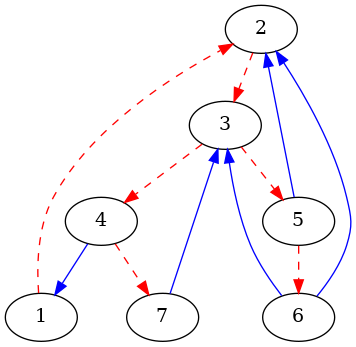
\includegraphics[width=6cm]{Figuras/G3.png}
\caption{Árbol generado en el recorrido primero en profundida en $G_{1, 1}$}
\label{figura:recorridoG1}
\end{figure}

\begin{figure}[H]
\centering
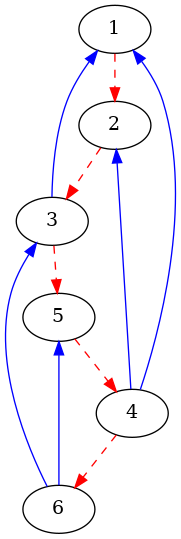
\includegraphics[width=3cm]{Figuras/G4.png}
\caption{Árbol generado en el recorrido primero en profundida en $G_{2}$}
\label{figura:recorridoG2}
\end{figure}

Calculamos los lowpt1 y lowpt2 de cada gráfica:
\begin{table}[H]
\begin{center}
\begin{tabular}{lll}
\toprule
vertice & lowpt1 & lowpt2 \\
\midrule
      1 &      1 &      1 \\
      2 &      1 &      2 \\
      3 &      1 &      2 \\
      4 &      1 &      3 \\
      5 &      2 &      3 \\
      6 &      2 &      3 \\
      7 &      3 &      5 \\
\bottomrule
\end{tabular}
\caption{Calculos de lowpt1 y lowpt2 en $G_{1,1}$}
\end{center}
\end{table}

\begin{table}[H]
\begin{center}
\begin{tabular}{lll}
\toprule
vertice & lowpt1 & lowpt2 \\
\midrule
      1 &      1 &      1 \\
      2 &      1 &      2 \\
      3 &      1 &      2 \\
      4 &      1 &      2 \\
      5 &      1 &      2 \\
      6 &      3 &      4 \\
\bottomrule
\end{tabular}
\caption{Calculos de lowpt1 y lowpt2 en $G_{2}$}
\end{center}
\end{table}

El ordenamiento de $\phi$ en $G_{1, 1}$ da el siguiente resultado:
\begin{center}
1: [2],\\
2: [3],\\
3: [4, 5],\\
4: [1, 7],\\
5: [6, 2],\\
6: [2, 3],\\
7: [3]
\end{center}

Los caminos generados de $G_{1, 1}$ son:
\begin{tabular}[t]{ll}
1: $1 \rightarrow 2 \rightarrow 3 \rightarrow 4 \hookrightarrow 1$ & 2: $4 \rightarrow 7 \hookrightarrow 3$ \\
3: $3 \rightarrow 5 \rightarrow 6 \hookrightarrow 2$ & 4: $6 \hookrightarrow 3$\\
5: $5 \hookrightarrow 2$ & \\
\end{tabular}\\

Solo hay pares de separación de tipo 1 en $G_{1, 1}$ los cuales son $(3, 4), (1, 3), (2, 3)$.

El ordenamiento de $\phi$ en $G_{2}$ da el siguiente resultado:
\begin{center}
1: [2],\\ 
2: [3],\\ 
3: [5, 1],\\ 
4: [1, 2, 6],\\ 
5: [4],\\ 
6: [3, 5]
\end{center}

Los caminos generados de $G_{2}$ son:
\begin{tabular}[t]{ll}
1: $1 \rightarrow 2 \rightarrow 3 \rightarrow 5 \rightarrow 4 \hookrightarrow 1$ & 2: $4 \hookrightarrow 2$ \\
3: $4 \rightarrow 6 \hookrightarrow 3$ & 4: $6 \hookrightarrow 5$\\
5: $3 \hookrightarrow 1$ & \\
\end{tabular}\\

Solo hay un par de separación de tipo 2 en $G_{2}$ el cual es $(3, 4)$.

\begin{figure}[H]
     \begin{subfigure}[b]{0.3\textwidth}
        \begin{minipage}{6cm}
        \centering% El subgrafo está centrado
        \begin{tikzpicture}[scale=.4]
        \GraphInit[vstyle=Normal]
        %
        \tikzset{VertexStyle/.append style={minimum size=1pt, inner sep=1pt}}
        \Vertex[L=\hbox{$3$},x=4.4318cm,y=0.0cm]{v0}
        \Vertex[L=\hbox{$4$},x=0.0cm,y=2.9366cm]{v1}
        \Vertex[L=\hbox{$7$},x=5.0cm,y=5.0cm]{v2}
        %
        \Edge[](v0)(v2)
        \Edge[](v1)(v2)
        \tikzstyle{EdgeStyle}=[color=red]
        \tikzset{LabelStyle/.style = {fill=white, scale=.6}}
        \Edge[label=$A$](v0)(v1)
        %
        \end{tikzpicture}
        \end{minipage}
        \caption{}
         \label{fig:f1}
     \end{subfigure}
     \begin{subfigure}[b]{0.3\textwidth}
        \begin{minipage}{6cm}
        \centering% El subgrafo está centrado
        \begin{tikzpicture}[scale=.4]
        \GraphInit[vstyle=Normal]
        %
        \tikzset{VertexStyle/.append style={minimum size=1pt, inner sep=1pt}}
        \Vertex[L=\hbox{$3$},x=0.0cm,y=0.0cm]{v0}
        \Vertex[L=\hbox{$4$},x=5.0cm,y=5.0cm]{v1}
        %
        \Edge[](v0)(v1)
        \tikzstyle{EdgeStyle}=[color=red]
        \tikzset{LabelStyle/.style = {fill=white, scale=.6}}
        \Edge[label=$A$, style={bend left}](v0)(v1)
        \Edge[label=$B$, style={bend right}](v0)(v1)
        %
        \end{tikzpicture}
        \end{minipage}
        \caption{}
         \label{fig:f1}
     \end{subfigure}
     \begin{subfigure}[b]{0.3\textwidth}
        \begin{minipage}{6cm}
        \centering% El subgrafo está centrado
        \begin{tikzpicture}[scale=.4]
        \GraphInit[vstyle=Normal]
        %
        \tikzset{VertexStyle/.append style={minimum size=1pt, inner sep=1pt}}
        \Vertex[L=\hbox{$1$},x=0.0cm,y=2.3583cm]{v0}
        \Vertex[L=\hbox{$3$},x=5.0cm,y=0.0cm]{v1}
        \Vertex[L=\hbox{$4$},x=4.8519cm,y=5.0cm]{v2}
        %
        \Edge[](v0)(v2)
        %
        \tikzstyle{EdgeStyle}=[color=red]
        \tikzset{LabelStyle/.style = {fill=white, scale=.6}}
        \Edge[label=$C$](v0)(v1)
        \Edge[label=$B$](v1)(v2)
        %
        \end{tikzpicture}
        \end{minipage}
        \caption{}
         \label{fig:f1}
     \end{subfigure}
     \begin{subfigure}[b]{0.3\textwidth}
        \begin{minipage}{6cm}
        \centering% El subgrafo está centrado
        \begin{tikzpicture}[scale=.4]
        \GraphInit[vstyle=Normal]
        %
        \tikzset{VertexStyle/.append style={minimum size=1pt, inner sep=1pt}}
        \Vertex[L=\hbox{$2$},x=2.2651cm,y=0.0cm]{v0}
        \Vertex[L=\hbox{$3$},x=0.0cm,y=2.6956cm]{v1}
        \Vertex[L=\hbox{$5$},x=2.7348cm,y=5.0cm]{v2}
        \Vertex[L=\hbox{$6$},x=5.0cm,y=2.3047cm]{v3}
        %
        \Edge[](v0)(v2)
        \Edge[](v0)(v3)
        \Edge[](v1)(v2)
        \Edge[](v1)(v3)
        \Edge[](v2)(v3)
        \tikzstyle{EdgeStyle}=[color=red]
        \tikzset{LabelStyle/.style = {fill=white, scale=.6}}
        \Edge[label=$D$](v0)(v1)
        %
        \end{tikzpicture}
        \end{minipage}
        \caption{}
         \label{fig:f1}
     \end{subfigure}
     \begin{subfigure}[b]{0.3\textwidth}
        \begin{minipage}{6cm}
        \centering% El subgrafo está centrado
        \begin{tikzpicture}[scale=.4]
        \GraphInit[vstyle=Normal]
        %
        \tikzset{VertexStyle/.append style={minimum size=1pt, inner sep=1pt}}
        \Vertex[L=\hbox{$2$},x=0.0cm,y=5.0cm]{v0}
        \Vertex[L=\hbox{$3$},x=5.0cm,y=0.0cm]{v1}
        %
        \Edge[](v0)(v1)
        \tikzstyle{EdgeStyle}=[color=red]
        \tikzset{LabelStyle/.style = {fill=white, scale=.6}}
        \Edge[label=$D$, style={bend left}](v0)(v1)
        \Edge[label=$E$, style={bend right}](v0)(v1)
        %
        \end{tikzpicture}
        \end{minipage}
        \caption{}
         \label{fig:f1}
     \end{subfigure}
     \begin{subfigure}[b]{0.3\textwidth}
        \begin{minipage}{6cm}
        \centering% El subgrafo está centrado
        \begin{tikzpicture}[scale=.4]
        \GraphInit[vstyle=Normal]
        %
        \tikzset{VertexStyle/.append style={minimum size=1pt, inner sep=1pt}}
        \Vertex[L=\hbox{$1$},x=4.1519cm,y=0.0cm]{v0}
        \Vertex[L=\hbox{$2$},x=0.0cm,y=3.1432cm]{v1}
        \Vertex[L=\hbox{$3$},x=5.0cm,y=5.0cm]{v2}
        %
        \Edge[](v0)(v1)
        \tikzstyle{EdgeStyle}=[color=red]
        \tikzset{LabelStyle/.style = {fill=white, scale=.6}}
        \Edge[label=$C$](v0)(v2)
        \Edge[label=$E$](v1)(v2)
        %
        \end{tikzpicture}
        \end{minipage}
        \caption{}
         \label{fig:f1}
     \end{subfigure}
     \caption{Componentes de separación de $G_{1, 1}$}
     \label{figura:componentesTriconexas}
\end{figure}

En el caso de $G_{2}$ los componentes de separación son iguales a las componentes triconexas finales.

Las componentes triconexas finales de las bigráficas:
\begin{figure}[H]
     \begin{subfigure}[b]{0.5\textwidth}
        \begin{minipage}{7cm}
        \centering% El subgrafo está centrado
        \begin{tikzpicture}[scale=.4]
        \GraphInit[vstyle=Normal]
        %
        \tikzset{VertexStyle/.append style={minimum size=1pt, inner sep=1pt}}
        \Vertex[L=\hbox{$3$},x=0.0cm,y=5.0cm]{v0}
        \Vertex[L=\hbox{$4$},x=5.0cm,y=3.5243cm]{v1}
        \Vertex[L=\hbox{$7$},x=1.3175cm,y=0.0cm]{v2}
        %
        \Edge[](v0)(v2)
        \Edge[](v1)(v2)
        \tikzstyle{EdgeStyle}=[color=red]
        \tikzset{LabelStyle/.style = {fill=white, scale=.6}}
        \Edge[label=$A$](v1)(v0)
        %
        \end{tikzpicture}
        \end{minipage}
        \caption{}
         \label{fig:f1}
     \end{subfigure}
     \begin{subfigure}[b]{0.5\textwidth}
        \begin{minipage}{7cm}
        \centering% El subgrafo está centrado
        \begin{tikzpicture}[scale=.4]
        \GraphInit[vstyle=Normal]
        %
        \tikzset{VertexStyle/.append style={minimum size=1pt, inner sep=1pt}}
        \Vertex[L=\hbox{$3$},x=5.0cm,y=0.0cm]{v0}
        \Vertex[L=\hbox{$4$},x=0.0cm,y=5.0cm]{v1}
        %
        \Edge[](v0)(v1)
        \tikzstyle{EdgeStyle}=[color=red]
        \tikzset{LabelStyle/.style = {fill=white, scale=.6}}
        \Edge[label=$A$, style={bend left}](v0)(v1)
        \Edge[label=$B$, style={bend right}](v0)(v1)
        %
        \end{tikzpicture}
        \end{minipage}
        \caption{}
         \label{fig:f1}
     \end{subfigure}
     \begin{subfigure}[b]{0.3\textwidth}
        \begin{minipage}{7cm}
        \centering% El subgrafo está centrado
        \begin{tikzpicture}[scale=.4]
        \GraphInit[vstyle=Normal]
        %
        \tikzset{VertexStyle/.append style={minimum size=1pt, inner sep=1pt}}
        \Vertex[L=\hbox{$1$},x=5.0cm,y=1.2919cm]{v0}
        \Vertex[L=\hbox{$2$},x=1.4292cm,y=0.0cm]{v1}
        \Vertex[L=\hbox{$3$},x=0.0cm,y=3.5377cm]{v2}
        \Vertex[L=\hbox{$4$},x=3.6225cm,y=5.0cm]{v3}
        %
        \Edge[](v0)(v1)
        \Edge[](v0)(v3)
        \tikzstyle{EdgeStyle}=[color=red]
        \tikzset{LabelStyle/.style = {fill=white, scale=.6}}
        \Edge[label=$E$](v1)(v2)
        \Edge[label=$B$](v2)(v3)
        %
        \end{tikzpicture}
        \end{minipage}
        \caption{}
         \label{fig:f1}
     \end{subfigure}
     \begin{subfigure}[b]{0.3\textwidth}
        \begin{minipage}{7cm}
        \centering% El subgrafo está centrado
        \begin{tikzpicture}[scale=.4]
        \GraphInit[vstyle=Normal]
        %
        \tikzset{VertexStyle/.append style={minimum size=1pt, inner sep=1pt}}
        \Vertex[L=\hbox{$2$},x=5.0cm,y=4.0504cm]{v0}
        \Vertex[L=\hbox{$3$},x=0.1743cm,y=5.0cm]{v1}
        \Vertex[L=\hbox{$5$},x=4.8257cm,y=0.0cm]{v2}
        \Vertex[L=\hbox{$6$},x=0.0cm,y=0.9496cm]{v3}
        %
        \Edge[](v0)(v2)
        \Edge[](v0)(v3)
        \Edge[](v1)(v2)
        \Edge[](v1)(v3)
        \Edge[](v2)(v3)
        \tikzstyle{EdgeStyle}=[color=red]
        \tikzset{LabelStyle/.style = {fill=white, scale=.6}}
        \Edge[label=$D$](v0)(v1)
        %
        \end{tikzpicture}
        \end{minipage}
        \caption{}
         \label{fig:f1}
     \end{subfigure}
     \begin{subfigure}[b]{0.3\textwidth}
        \begin{minipage}{7cm}
        \centering% El subgrafo está centrado
        \begin{tikzpicture}[scale=.4]
        \GraphInit[vstyle=Normal]
        %
        \tikzset{VertexStyle/.append style={minimum size=1pt, inner sep=1pt}}
        \Vertex[L=\hbox{$2$},x=5.0cm,y=0.0cm]{v0}
        \Vertex[L=\hbox{$3$},x=0.0cm,y=5.0cm]{v1}
        %
        \Edge[](v0)(v1)
        \tikzstyle{EdgeStyle}=[color=red]
        \tikzset{LabelStyle/.style = {fill=white, scale=.6}}
        \Edge[label=$D$, style={bend left}](v0)(v1)
        \Edge[label=$E$, style={bend right}](v0)(v1)
        %
        \end{tikzpicture}
        \end{minipage}
        \caption{}
         \label{fig:f1}
     \end{subfigure}
     \caption{Componentes triconexas de $G_{1,1}$}
     \label{figura:componentesTriconexas}
\end{figure}

\begin{figure}[H]
    \begin{subfigure}[b]{0.5\textwidth}
        \begin{minipage}{7cm}
        \centering% El subgrafo está centrado
        \begin{tikzpicture}[scale=.4]
        \GraphInit[vstyle=Normal]
        %
        \tikzset{VertexStyle/.append style={minimum size=1pt, inner sep=1pt}}
        \Vertex[L=\hbox{$3$},x=2.7617cm,y=5.0cm]{v0}
        \Vertex[L=\hbox{$4$},x=5.0cm,y=2.3416cm]{v1}
        \Vertex[L=\hbox{$5$},x=0.0cm,y=2.8439cm]{v2}
        \Vertex[L=\hbox{$6$},x=2.4111cm,y=0.0cm]{v3}
        %
        \Edge[](v2)(v3)
        \Edge[](v0)(v2)
        \Edge[](v0)(v3)
        \Edge[](v1)(v2)
        \Edge[](v1)(v3)
        \tikzstyle{EdgeStyle}=[color=red]
        \tikzset{LabelStyle/.style = {fill=white, scale=.6}}
        \Edge[label=$A$](v0)(v1)
        %
        \end{tikzpicture}
        \end{minipage}
        \caption{}
         \label{fig:f1}
     \end{subfigure}
     \begin{subfigure}[b]{0.5\textwidth}
        \begin{minipage}{7cm}
        \centering% El subgrafo está centrado
        \begin{tikzpicture}[scale=.4]
        \GraphInit[vstyle=Normal]
        %
        \tikzset{VertexStyle/.append style={minimum size=1pt, inner sep=1pt}}
        \Vertex[L=\hbox{$1$},x=4.7286cm,y=5.0cm]{v0}
        \Vertex[L=\hbox{$2$},x=5.0cm,y=0.1367cm]{v1}
        \Vertex[L=\hbox{$3$},x=0.0cm,y=4.8796cm]{v2}
        \Vertex[L=\hbox{$4$},x=0.3559cm,y=0.0cm]{v3}
        %
        \Edge[](v0)(v1)
        \Edge[](v0)(v2)
        \Edge[](v0)(v3)
        \Edge[](v1)(v2)
        \Edge[](v1)(v3)
        \tikzstyle{EdgeStyle}=[color=red]
        \tikzset{LabelStyle/.style = {fill=white, scale=.6}}
        \Edge[label=$A$](v2)(v3)
        %
        \end{tikzpicture}
        \end{minipage}
        \caption{}
         \label{fig:f1}
     \end{subfigure}
     \caption{Componentes triconexas de $G_{2}$}
     \label{figura:componentesTriconexas1}
\end{figure}

Obtenemos ahora la bigráfica original y aplicamos el criterio para decidir si la arista virtual es solida o punteada.
\begin{figure}[H]
     \begin{subfigure}[b]{0.5\textwidth}
        \begin{minipage}{7cm}
        \centering% El subgrafo está centrado
        \begin{tikzpicture}[scale=.6]
        \GraphInit[vstyle=Normal]
        %
        \tikzset{VertexStyle/.append style={minimum size=1pt, inner sep=1pt}}
        \Vertex[L=\hbox{$2$},x=4.01cm,y=2.517cm]{v1}
        \Vertex[L=\hbox{$3$},x=1.7633cm,y=2.517cm]{v2}
        \Vertex[L=\hbox{$5$},x=1.7633cm,y=4.5228cm]{v4}
        \Vertex[L=\hbox{$6$},x=4.01cm,y=4.5228cm]{v5}
        %
        \Edge[](v1)(v4)
        \Edge[](v1)(v5)
        \Edge[](v2)(v4)
        \Edge[](v2)(v5)
        \Edge[style=dashed](v4)(v5)
        \Edge[style=dashed](v1)(v2)
        %
        \end{tikzpicture}
        \end{minipage}
        \caption{}
         \label{fig:f1}
     \end{subfigure}
     \begin{subfigure}[b]{0.5\textwidth}
        \begin{minipage}{7cm}
        \centering% El subgrafo está centrado
        \begin{tikzpicture}[scale=.6]
        \GraphInit[vstyle=Normal]
        %
        \tikzset{VertexStyle/.append style={minimum size=1pt, inner sep=1pt}}
        \Vertex[L=\hbox{$2$},x=4.31cm,y=3.2064cm]{v1}
        \Vertex[L=\hbox{$3$},x=1.7633cm,y=2.517cm]{v2}
        %
        \Edge[](v1)(v2)
        %
        \end{tikzpicture}
        \end{minipage}
        \caption{}
         \label{fig:f1}
     \end{subfigure}
     \begin{subfigure}[b]{0.3\textwidth}
        \begin{minipage}{7cm}
        \centering% El subgrafo está centrado
        \begin{tikzpicture}[scale=.6]
        \GraphInit[vstyle=Normal]
        %
        \tikzset{VertexStyle/.append style={minimum size=1pt, inner sep=1pt}}
        \Vertex[L=\hbox{$3$},x=1.3633cm,y=2.517cm]{v2}
        \Vertex[L=\hbox{$4$},x=2.3604cm,y=0.0cm]{v3}
        \Vertex[L=\hbox{$7$},x=0.0cm,y=0.0cm]{v6}
        %
        \Edge[](v2)(v3)
        \Edge[](v2)(v6)
        \Edge[style=dashed](v3)(v6)
        %
        \end{tikzpicture}
        \end{minipage}
        \caption{}
         \label{fig:f1}
     \end{subfigure}
     \begin{subfigure}[b]{0.3\textwidth}
        \begin{minipage}{7cm}
        \centering% El subgrafo está centrado
        \begin{tikzpicture}[scale=.6]
        \GraphInit[vstyle=Normal]
        %
        \tikzset{VertexStyle/.append style={minimum size=1pt, inner sep=1pt}}
        \Vertex[L=\hbox{$3$},x=1.7633cm,y=2.317cm]{v2}
        \Vertex[L=\hbox{$4$},x=2.3604cm,y=0.0cm]{v3}
        %
        \Edge[](v2)(v3)
        %
        \end{tikzpicture}
        \end{minipage}
        \caption{}
         \label{fig:f1}
     \end{subfigure}
     \begin{subfigure}[b]{0.3\textwidth}
        \begin{minipage}{7cm}
        \centering% El subgrafo está centrado
        \begin{tikzpicture}[scale=.6]
        \GraphInit[vstyle=Normal]
        %
        \tikzset{VertexStyle/.append style={minimum size=1pt, inner sep=1pt}}
        \Vertex[L=\hbox{$1$},x=5.0cm,y=0.0cm]{v0}
        \Vertex[L=\hbox{$2$},x=5.0cm,y=2.517cm]{v1}
        \Vertex[L=\hbox{$3$},x=2.3604cm,y=2.517cm]{v2}
        \Vertex[L=\hbox{$4$},x=2.3604cm,y=0.0cm]{v3}
        %
        \Edge[](v0)(v1)
        \Edge[](v0)(v3)
        \Edge[](v1)(v2)
        \Edge[style=dashed](v2)(v3)
        %
        \end{tikzpicture}
        \end{minipage}
        \caption{}
         \label{fig:f1}
     \end{subfigure}
     \caption{Componentes triconexas de $G_{1,1}$}
     \label{figura:componentesTriconexas}
\end{figure}

De el capitulo 2 sabemos que estas gráficas excepto (e) son $\DynA$-bloques.

\begin{figure}[H]
    \begin{subfigure}[b]{0.5\textwidth}
        \begin{minipage}{7cm}
        \centering% El subgrafo está centrado
        \begin{tikzpicture}[scale=.6]
        \GraphInit[vstyle=Normal]
        %
        \tikzset{VertexStyle/.append style={minimum size=1pt, inner sep=1pt}}
        \Vertex[L=\hbox{$3$},x=2.8524cm,y=2.0745cm]{v2}
        \Vertex[L=\hbox{$4$},x=0.3702cm,y=2.0745cm]{v3}
        \Vertex[L=\hbox{$5$},x=2.8524cm,y=4.8114cm]{v4}
        \Vertex[L=\hbox{$6$},x=0.3702cm,y=4.8114cm]{v5}
        %
        \Edge[](v2)(v3)
        \Edge[](v2)(v4)
        \Edge[style=dashed](v2)(v5)
        \Edge[](v4)(v5)
        \Edge[style=dashed](v4)(v3)
        \Edge[](v3)(v5)
        \Edge[](v2)(v3)
        %
        \end{tikzpicture}
        \end{minipage}
        \caption{}
         \label{fig:f1}
     \end{subfigure}
     \begin{subfigure}[b]{0.5\textwidth}
        \begin{minipage}{7cm}
        \centering% El subgrafo está centrado
        \begin{tikzpicture}[scale=.6]
        \GraphInit[vstyle=Normal]
        %
        \tikzset{VertexStyle/.append style={minimum size=1pt, inner sep=1pt}}
        \Vertex[L=\hbox{$1$},x=4.4008cm,y=0.0cm]{v0}
        \Vertex[L=\hbox{$2$},x=4.4008cm,y=2.7015cm]{v1}
        \Vertex[L=\hbox{$3$},x=1.8549cm,y=2.7015cm]{v2}
        \Vertex[L=\hbox{$4$},x=1.8549cm,y=0.0cm]{v3}
        %
        \Edge[style=dashed](v0)(v1)
        \Edge[](v0)(v2)
        \Edge[](v1)(v2)
        \Edge[](v3)(v1)
        \Edge[](v3)(v0)
        \Edge[style=dashed](v2)(v3)
        %
        \end{tikzpicture}
        \end{minipage}
        \caption{}
         \label{fig:f1}
     \end{subfigure}
     \caption{Componentes triconexas de $G_{2}$}
     \label{figura:componentesTriconexas1}
\end{figure}






\chapter{Componentes triconexas en un bigráfo $\DynD_{n}$.}

\section{Algoritmo para encontrar componentes triconexas de un bigráfo de tipo $\DynD_{n}$}


\begin{appendix}


\end{appendix}
\addcontentsline{toc}{chapter}{\numberline{}Bibliograf\'{\i}a}
\renewcommand{\refname}{Bibliografía}
\bibliographystyle{apalike}
\typeout{}
\bibliography{BibliMSC}
\end{document}